%%%%%%%%%%%%%%%%%%%%%%%%%%%%%%%%%%%%% 
%% LE2I beamer template
%% Guillaume Lemaitre, October 2014
%%%%%%%%%%%%%%%%%%%%%%%%%%%%%%%%%%%%% 

\documentclass{beamer}

\usepackage[utf8]{inputenc}
\usepackage[T1]{fontenc} 
\usefonttheme[onlymath]{serif}
\usetheme{le2i} 

%% The amssymb package provides various useful mathematical symbols
\usepackage{amssymb}
%% The amsthm package provides extended theorem environments
\usepackage{amsthm}
%% amsmath for math environment
\usepackage{amsmath}

\DeclareMathOperator*{\argmin}{arg\,min}
\DeclareMathOperator*{\argmax}{arg\,max}
\DeclareMathOperator*{\sign}{sign}

\usepackage{siunitx}

\makeatletter
\newcommand{\srcsize}{\@setfontsize{\srcsize}{5pt}{5pt}}
\makeatother

%% Bibtex information
\usepackage[style=verbose,autocite=footnote,maxnames=2,babel=hyphen,hyperref=true,abbreviate=true,backend=biber,mcite]{biblatex}
\addbibresource{literature.bib}
\setbeamertemplate{footnote}{%
  \tiny%
  \parindent 1em\noindent%
  \raggedright
  \hbox to 1.8em{\hfil\insertfootnotemark}\insertfootnotetext\par%
}%
\setlength\footnotesep{0pt}

%% figure package
\usepackage{epsf,graphicx}
\usepackage{epstopdf}
\usepackage{subfigure}
\usepackage{transparent}
\usepackage{caption}
\captionsetup{font=scriptsize,labelfont=scriptsize,labelformat=empty}
\setbeamertemplate{caption}{\raggedright\insertcaption\par}

%% In order to draw some graphs
\usepackage{tikz,xifthen}
\usepackage{tikz-qtree}
\usepackage{adjustbox}
\usetikzlibrary{decorations.pathmorphing}
\usetikzlibrary{fit}
\usetikzlibrary{backgrounds}
\usetikzlibrary{shapes,arrows,shadows}
\usetikzlibrary{calc,decorations.pathreplacing,decorations.markings,positioning}
\usetikzlibrary{snakes,decorations.text,shapes,patterns}
% \usepackage{scalefnt,lmodern,booktabs}

\usepackage{booktabs}
\usepackage{multirow}

\newcommand*{\tikzbullet}[2]{%
   \setbox0=\hbox{\strut}%
   \begin{tikzpicture}
     \useasboundingbox (-0.25em,0.25em) rectangle (.25em,\ht0);
     \filldraw[draw=#1,fill=#2] (0,0.5\ht0) circle[radius=.25em];
   \end{tikzpicture}%
}

%% Package for cross and tick symbols
\usepackage{pifont}
\newcommand{\tick}{\color{green!60!black!80}\ding{51}}
\newcommand{\cross}{\color{red!60!black!80}\ding{55}}

\title{Computer-Aided Diagnosis for Prostate Cancer using mp-MRI}
\author[Guillaume Lema\^itre]{Guillaume Lema\^itre}
\date{PhD Defence \\ 28\textsuperscript{th} November 2016}

\institute{Universitat de Girona - ViCOROB \\ Universit\'e de Bourgogne Franche-Comt\'e - LE2I} 

\newenvironment<>{redblock}[1]{%
  \begin{actionenv}#2%
    \def\insertblocktitle{#1}%
    \par%
    \mode<presentation>{%
      \setbeamercolor{block title}{fg=nicewhite,bg=red!75!black}
      \setbeamercolor{block body}{fg=niceblack,bg=red!20}
    }%
    \usebeamertemplate{block begin}}
  {\par\usebeamertemplate{block end}\end{actionenv}}

\newenvironment<>{greenblock}[1]{%
  \begin{actionenv}#2%
    \def\insertblocktitle{#1}%
    \par%
    \mode<presentation>{%
      \setbeamercolor{block title}{fg=nicewhite,bg=green!40!black}
      \setbeamercolor{block body}{fg=niceblack,bg=green!20}
    }%
    \usebeamertemplate{block begin}}
  {\par\usebeamertemplate{block end}\end{actionenv}}

%% Uncomment if you want to avoid thousand of bullet inside the menu
% \usepackage{etoolbox}
% \makeatletter
% \patchcmd{\slideentry}{\advance\beamer@xpos by1\relax}{}{}{}
% \def\beamer@subsectionentry#1#2#3#4#5{\advance\beamer@xpos by1\relax}%
% \makeatother

\setbeamercovered{transparent}

\usepackage{environ}% Required for \NewEnviron, i.e. to read the whole body of the environment
\makeatletter

\newcounter{acolumn}%  Number of current column
\newlength{\acolumnmaxheight}%   Maximum column height


% `column` replacement to measure height
\newenvironment{@acolumn}[1]{%
    \stepcounter{acolumn}%
    \begin{lrbox}{\@tempboxa}%
    \begin{minipage}{#1}%
}{%
    \end{minipage}
    \end{lrbox}
    \@tempdimc=\dimexpr\ht\@tempboxa+\dp\@tempboxa\relax
    % Save height of this column:
    \expandafter\xdef\csname acolumn@height@\roman{acolumn}\endcsname{\the\@tempdimc}%
    % Save maximum height
    \ifdim\@tempdimc>\acolumnmaxheight
        \global\acolumnmaxheight=\@tempdimc
    \fi
}

% `column` wrapper which sets the height beforehand
\newenvironment{@@acolumn}[1]{%
    \stepcounter{acolumn}%
    % The \autoheight macro contains a \vspace macro with the maximum height minus the natural column height
    \edef\autoheight{\noexpand\vspace*{\dimexpr\acolumnmaxheight-\csname acolumn@height@\roman{acolumn}\endcsname\relax}}%
    % Call original `column`:
    \orig@column{#1}%
}{%
    \endorig@column
}

% Save orignal `column` environment away
\let\orig@column\column
\let\endorig@column\endcolumn

% `columns` variant with automatic height adjustment
\NewEnviron{acolumns}[1][]{%
    % Init vars:
    \setcounter{acolumn}{0}%
    \setlength{\acolumnmaxheight}{0pt}%
    \def\autoheight{\vspace*{0pt}}%
    % Set `column` environment to special measuring environment
    \let\column\@acolumn
    \let\endcolumn\end@acolumn
    \BODY% measure heights
    % Reset counter for second processing round
    \setcounter{acolumn}{0}%
    % Set `column` environment to wrapper
    \let\column\@@acolumn
    \let\endcolumn\end@@acolumn
    % Finally process columns now for real
    \begin{columns}[#1]%
        \BODY
    \end{columns}%
}
\makeatother


\begin{document}

% \setbeamertemplate{caption}{\raggedright\insertcaption\par}

{
  \setbeamertemplate{footline}{}
  % Show the title page
  \begin{frame}
    \titlepage
  \end{frame}
}
 
% Show the table of contents
\begin{frame}
  \tableofcontents[sectionstyle=show,subsectionstyle=hide,subsubsectionstyle=hide]
\end{frame}

\section{Introduction}

\begin{frame}
    \tableofcontents[currentsection,currentsubsection,subsectionstyle=show/show/hide]
\end{frame}

\subsection{Motivations}

\begin{frame}
  \frametitle{Introduction}
  \framesubtitle{Motivations}
  \begin{block}{\small Statistics}
    \begin{figure}%
      \centering
      \hspace*{\fill}%
      \subfigure[][\tiny \# of cancer cases]{%
        \label{fig:stat1a}%
        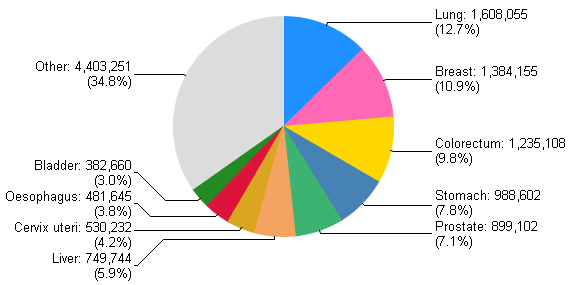
\includegraphics[width=.4\textwidth]{./images/statistics/repartitionCancerIncidence.png}}%
      \hfill%
      \subfigure[][\tiny \# of cancer deaths]{%
        \label{fig:stat1b}%
        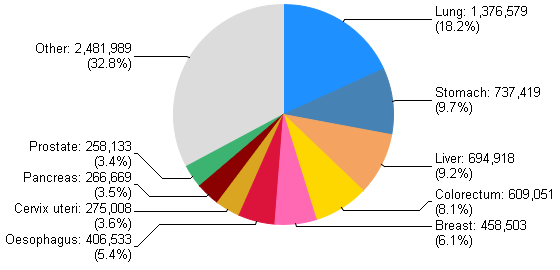
\includegraphics[width=.4\textwidth]{./images/statistics/repartitionCancerDeaths.png}}%
      \hspace*{\fill}%
      \label{fig:stat1}%
      % \caption{Statistics regarding cancer in 2008~\footnotemark}
    \end{figure}
  \end{block}
  \begin{block}{\small Implications, image source\footnotemark}\scriptsize
    \begin{itemize}
    \item 2\textsuperscript{nd} most frequently diagnosed men cancer
    \item Accounting for $7.1\%$ of overall cancers diagnosed
    \item Accounting for $3.4\%$ of overall cancers death
    \end{itemize}
  \end{block}
  \footcitetext{Ferlay2010}
\end{frame}

\subsection{The prostate organ}

\begin{frame}
  \frametitle{Introduction}
  \framesubtitle{The prostate organ}
  \begin{block}{\small Anatomy}
    \begin{figure}%
      \centering
      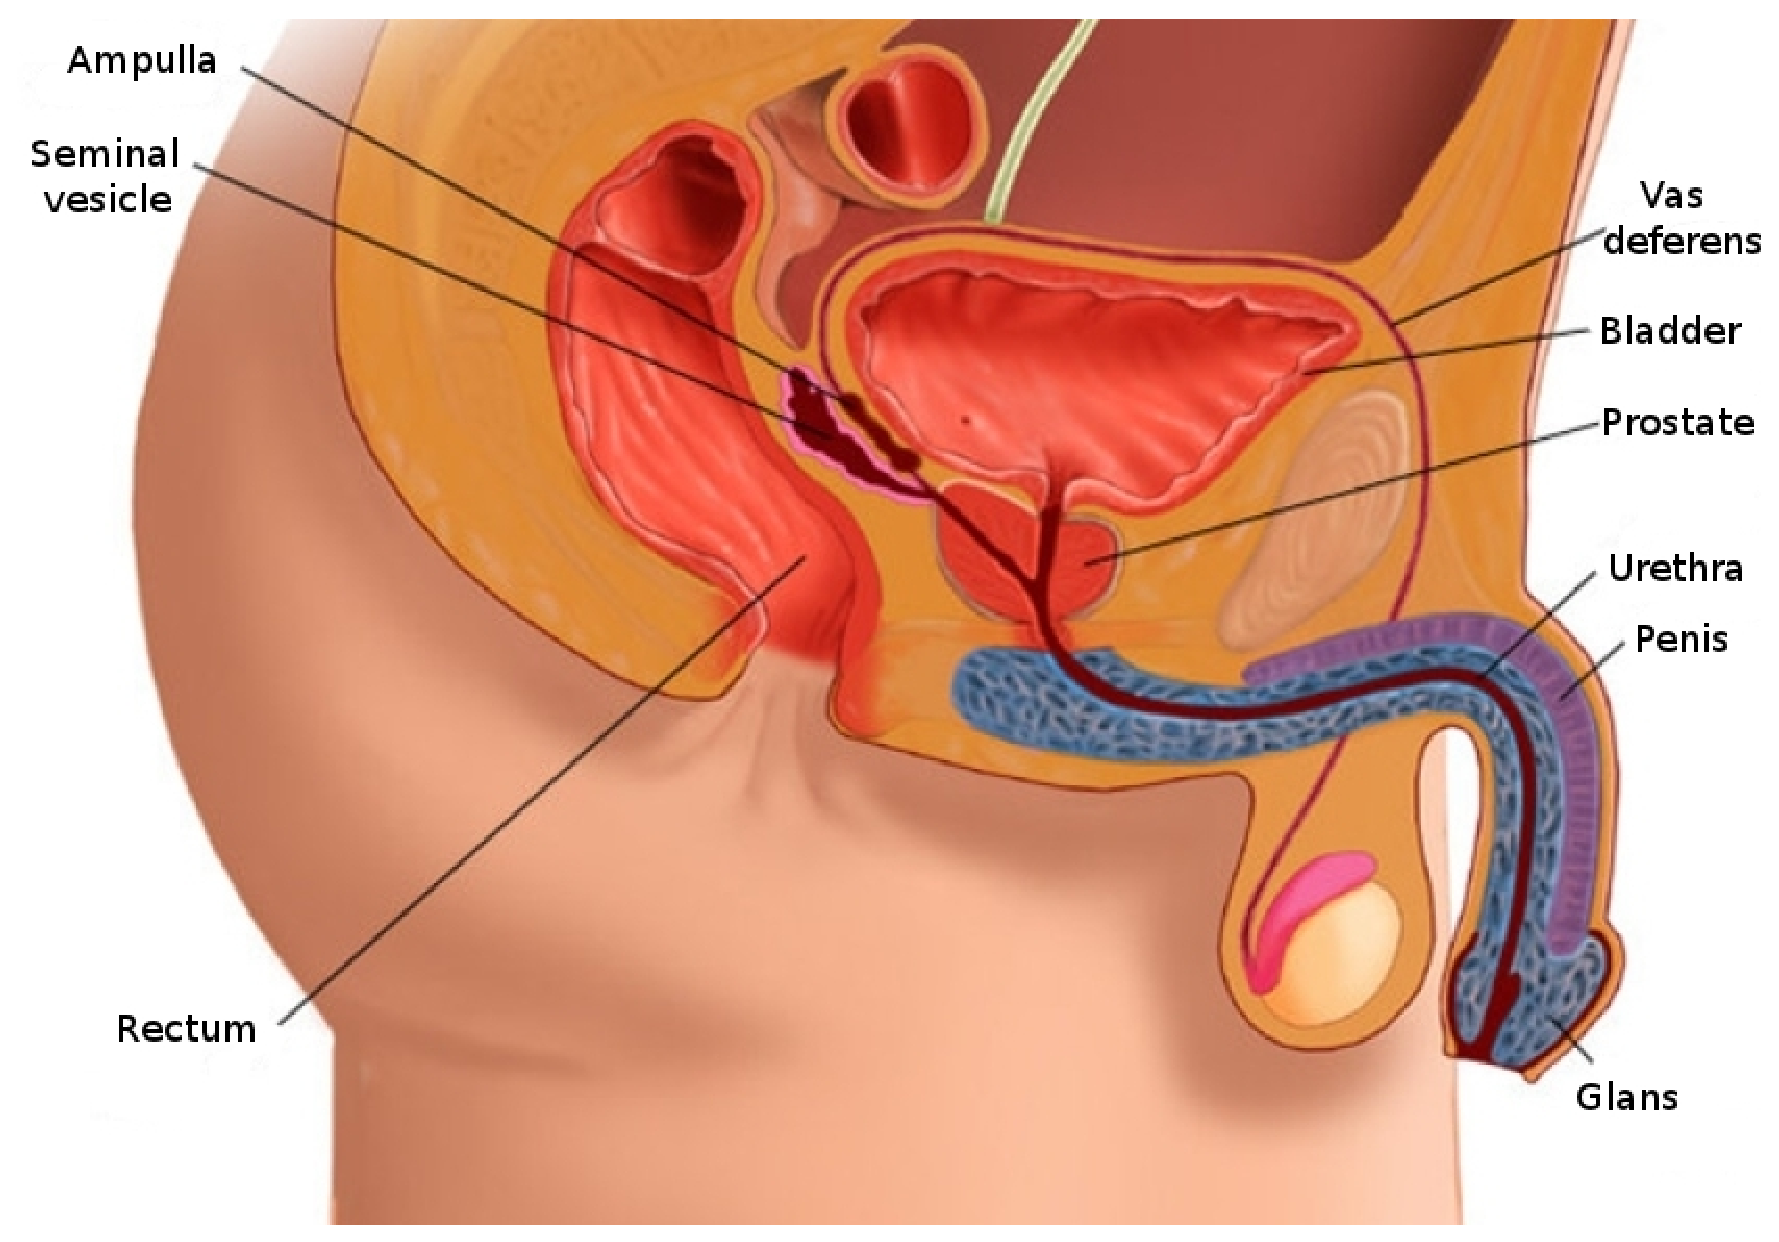
\includegraphics[height=.3\textheight]{./images/anatomy/prostate2D.eps}
      \caption{\tiny Localization of the prostate organ, image source\footnotemark}
    \end{figure}
  \end{block}
  \begin{block}{\small Characteristics}\scriptsize
    \begin{itemize}
    \item Height: \SI{3}{\cm}
    \item Depth: \SI{2.5}{\cm}
    \item Weight: \SIrange{7}{16}{\g}
    \end{itemize}
  \end{block}
  \footcitetext{Geckomedia2011}
\end{frame}

\begin{frame}
  \frametitle{Introduction}
  \framesubtitle{The prostate organ}
  \begin{block}{\small Anatomy}
    \begin{figure}%
      \centering
      \hspace*{\fill}%
      \subfigure[][\tiny Transverse plane]{%
        \label{fig:stat1a}%
        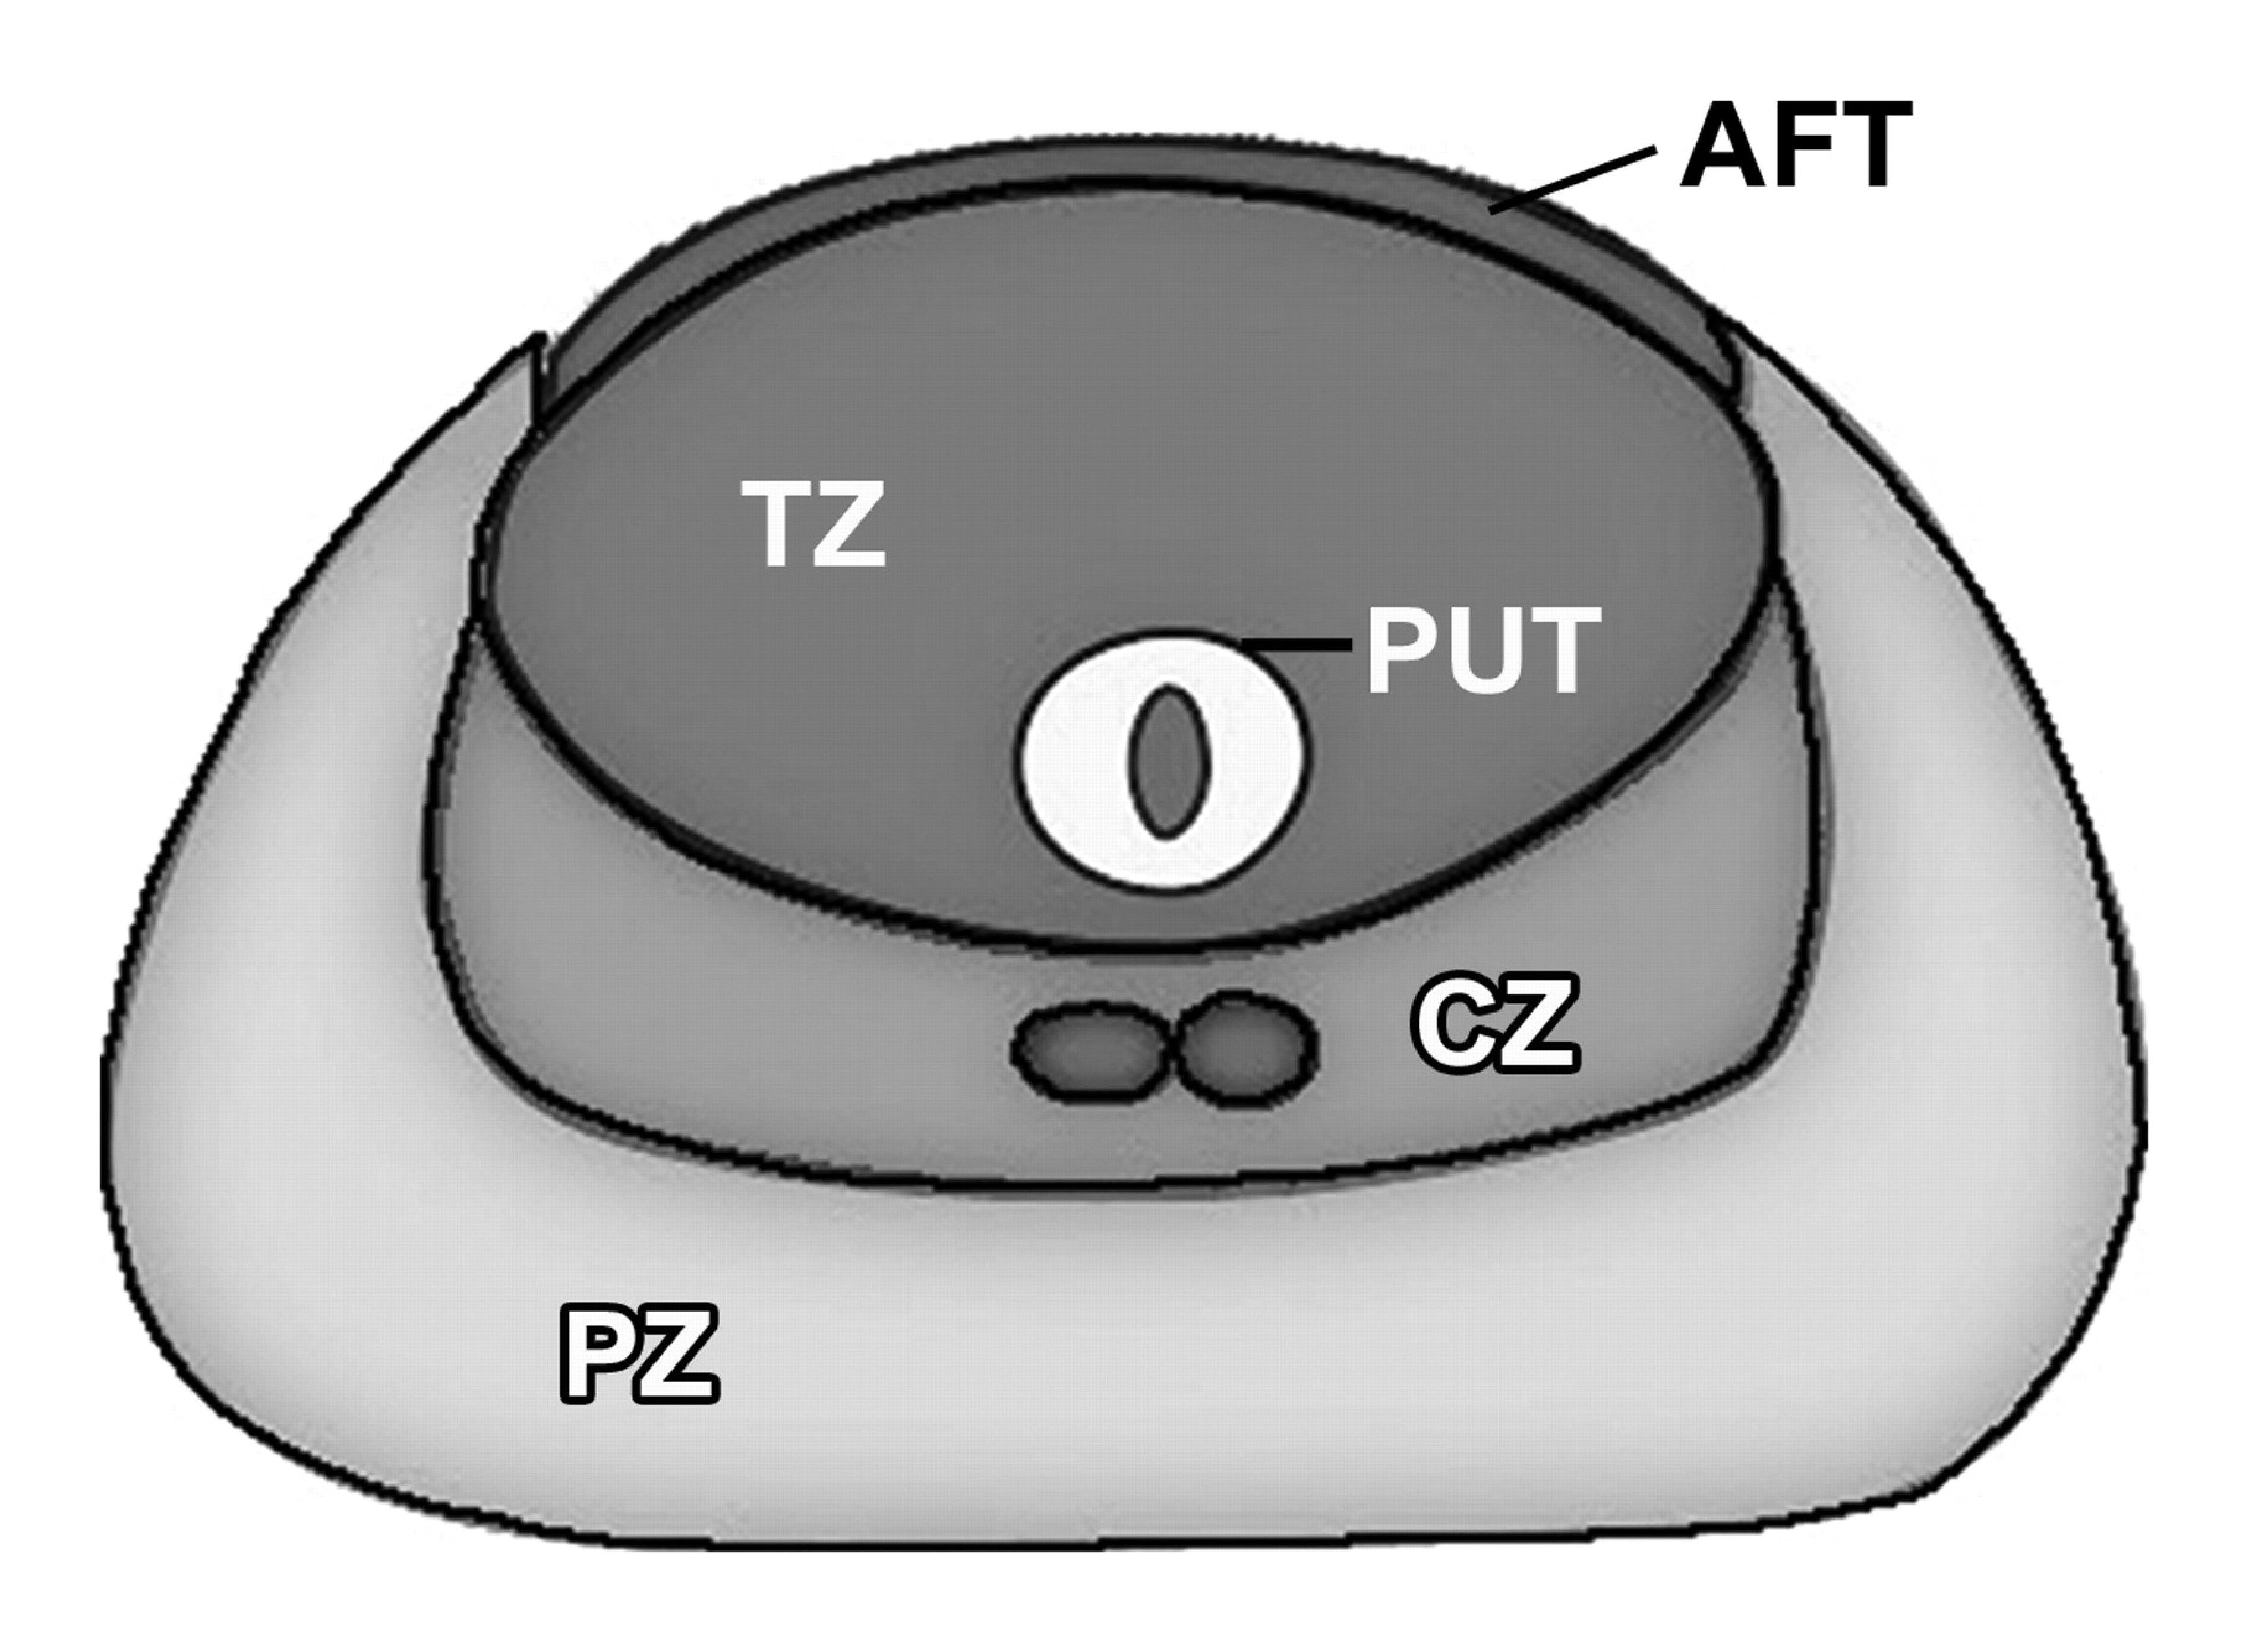
\includegraphics[height=.28\textheight]{./images/anatomy/prostateTransverse.eps}}%
      \hfill%
      \subfigure[][\tiny Sagittal plane]{%
        \label{fig:stat1b}%
        \includegraphics[height=.35\textheight]{./images/anatomy/prostateSagital.eps}}%
      \hspace*{\fill}%
      \caption{\tiny Prostate zones - AFT: anterior fibromuscular tissue, CZ: central zone, ED: ejaculatory duct, NVB: neurovascular bundle, PUT: periurethral tissue, PZ: peripheral zone, U: urethra, TZ: transitional zone, B: base, M: median, A: apex; image source\footnotemark}
      \label{fig:stat1}%
    \end{figure}
  \end{block}
  \footcitetext{Choi2007}
\end{frame}

\subsection{Prostate carcinoma}

\begin{frame}
  \frametitle{Introduction}
  \framesubtitle{Prostate carcinoma (CaP)}
  \begin{center}
    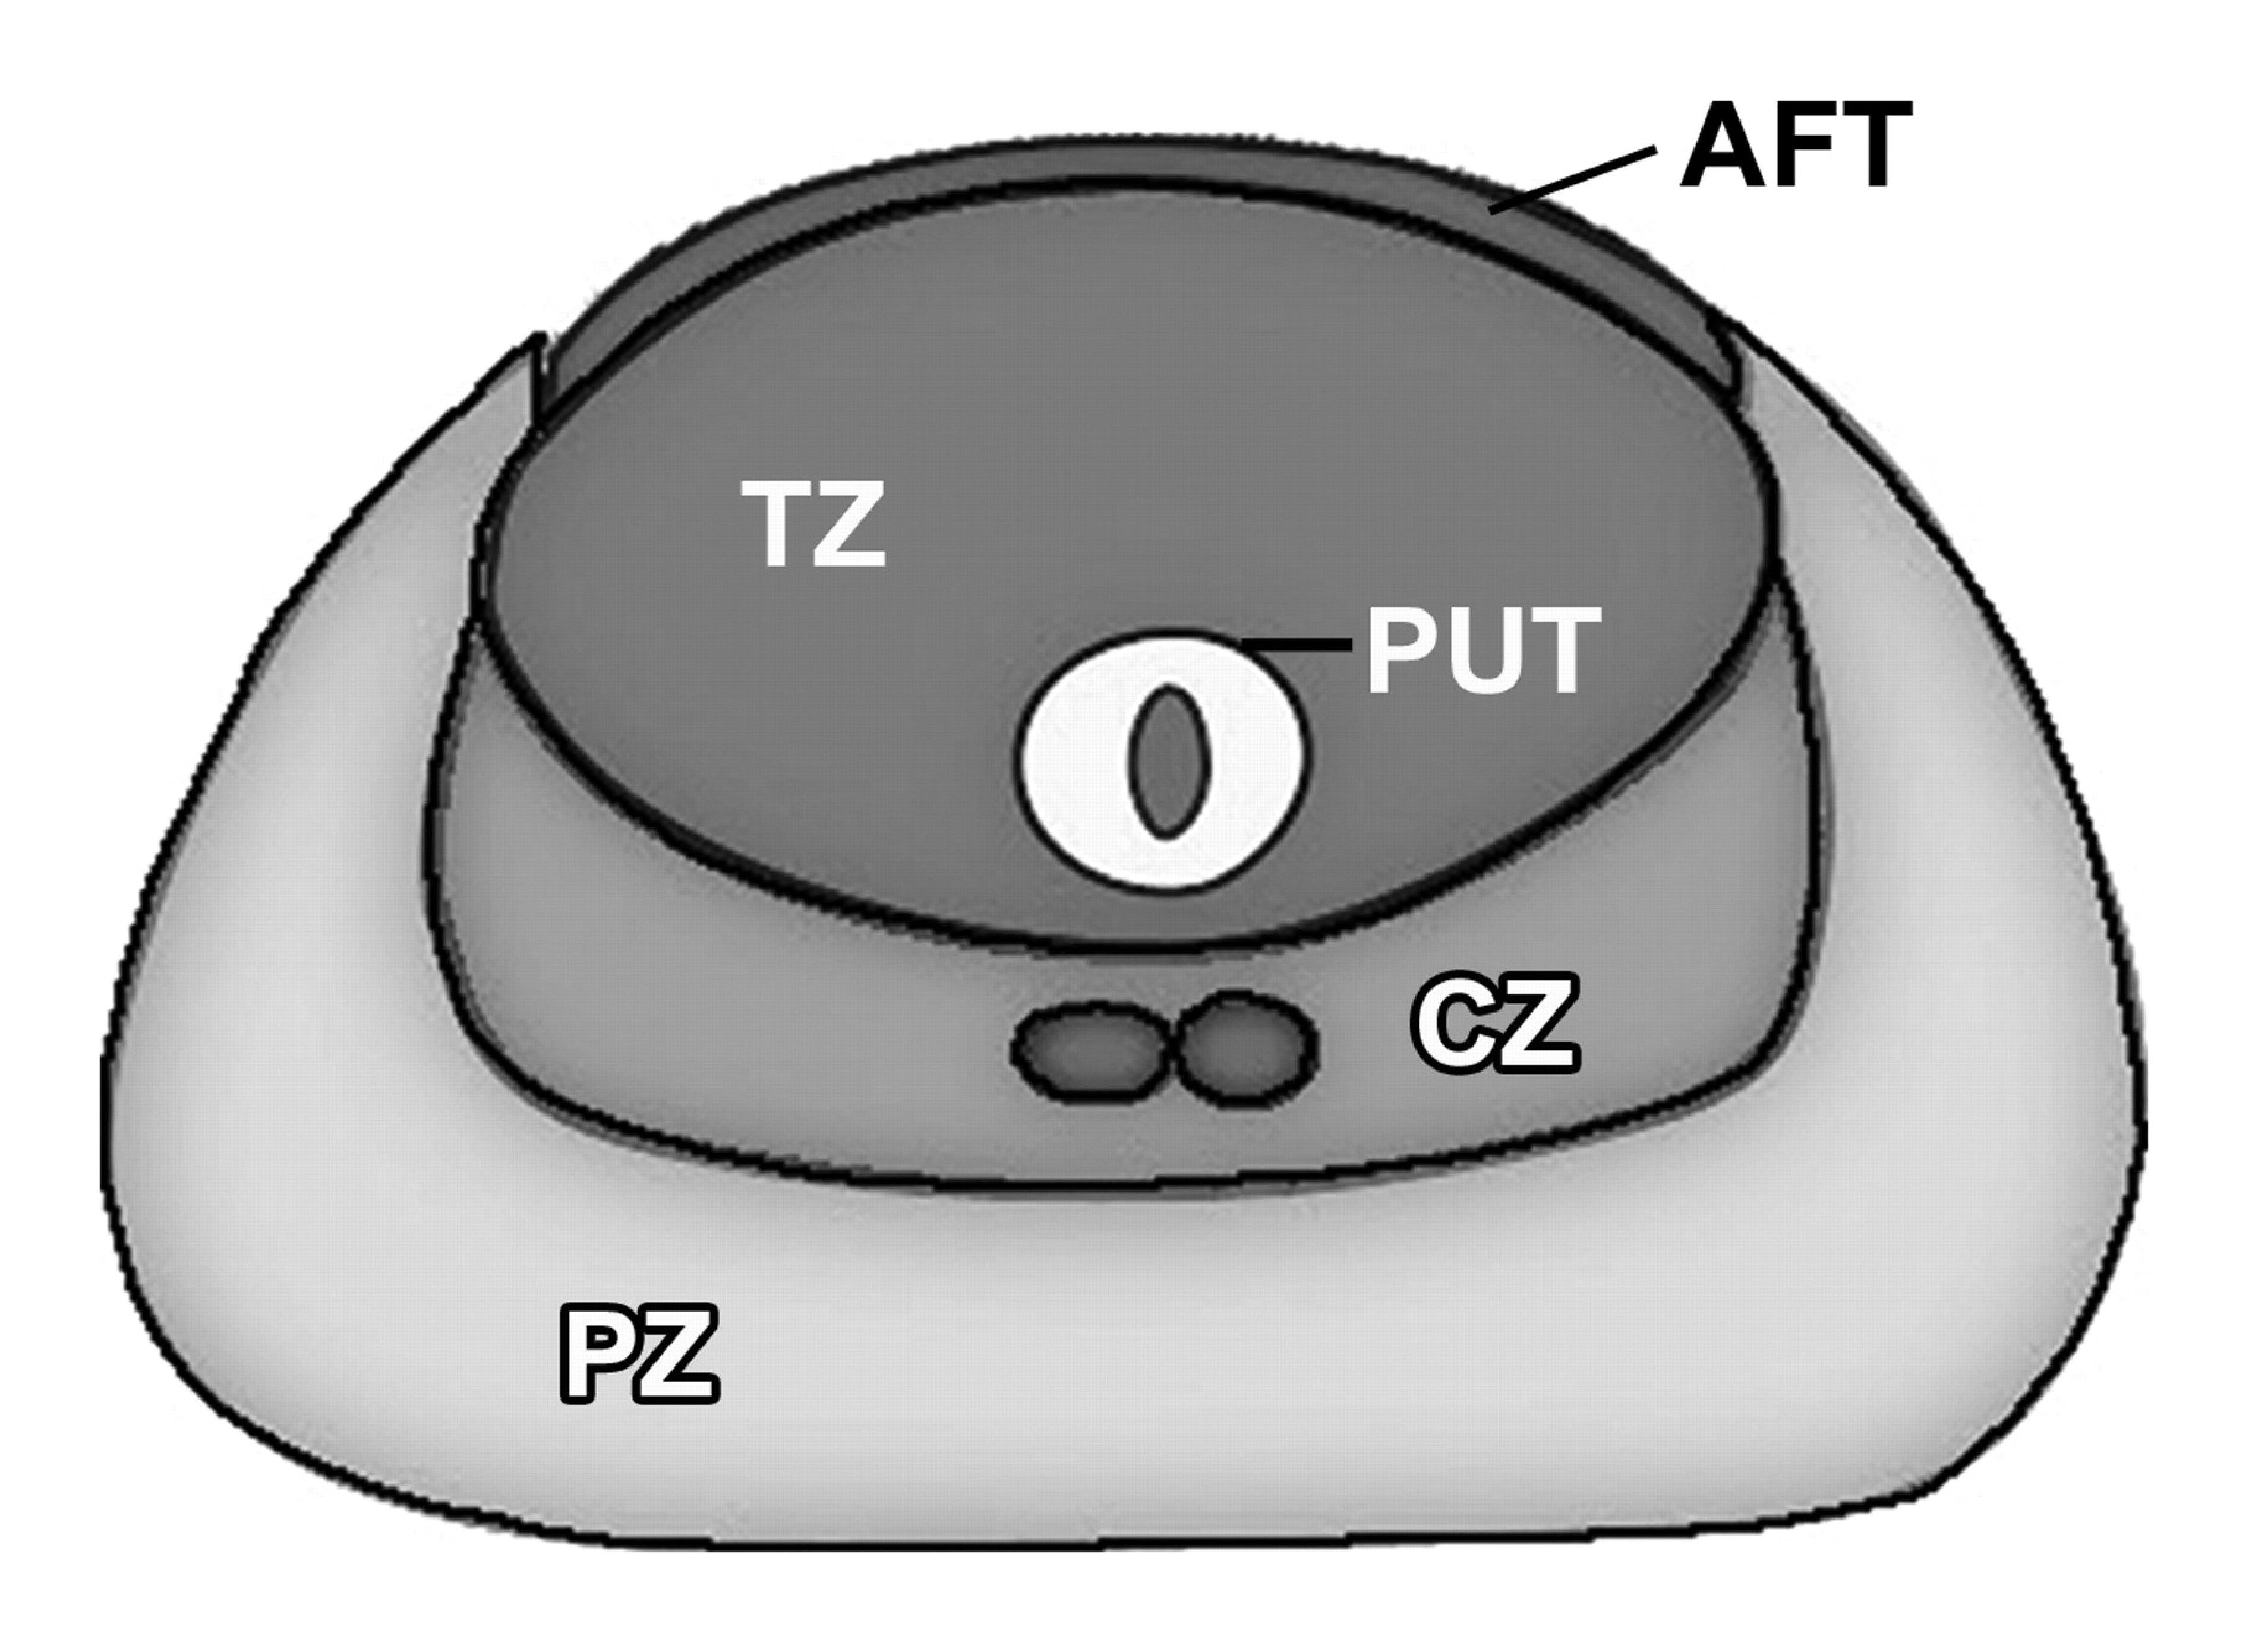
\includegraphics[height=.25\textheight]{./images/anatomy/prostateTransverse.eps}
  \end{center}
  \begin{columns}
    \begin{column}{0.45\textwidth}
      \begin{block}{\small CaP development}
        \begin{itemize}\scriptsize
        \item Slow-growing $\rightarrow$ \SI{85}{\percent}
        \item Fast-growing $\rightarrow$ \SI{15}{\percent}
        \item CaPs in CG are more aggressive
        \end{itemize}
      \end{block}
    \end{column}
    \begin{column}{0.45\textwidth}
      \begin{block}{\small Zonal predisposition}
        \begin{itemize}\scriptsize
        \item PZ $\rightarrow$ \SIrange{70}{80}{\percent}
        \item TZ $\rightarrow$ \SIrange{10}{20}{\percent}
        \item CG $\rightarrow$ \SI{5}{\percent}
        \end{itemize}
      \end{block}
    \end{column}
  \end{columns}
  \begin{greenblock}{\small Goals}
    \begin{itemize}\scriptsize
    \item Detect CaP
    \item Distinguish slow- from fast-growing CaP
    \item Active surveillance \emph{vs.} prostatectomy/other treatments
    \end{itemize}
  \end{greenblock}
\end{frame}

\subsection{Screening}

\begin{frame}
  \frametitle{Introduction}
  \framesubtitle{Screening}
  \begin{columns}
    \begin{column}{0.5\textwidth}
      \begin{block}<1->{\small Prostate-specific antigen}
        \begin{itemize}\scriptsize
        \item<1-> $>$ \SI{10}{\nano\gram\per\milli\liter} $\rightarrow$ biopsy
        \item<2-> From \SIrange{4}{10}{\nano\gram\per\milli\liter}
          \begin{itemize}\scriptsize
          \item[$\rightarrow$] $\frac{\text{\tikzbullet{gray}{orangeubfc}}}{\text{\tikzbullet{gray}{orangeubfc}}\  +\  \text{\tikzbullet{gray}{blueubfc}}} > 15 \% \rightarrow$ biopsy
          \end{itemize}
        \item[\cross]<3-> Not reliable
        \end{itemize}
      \end{block}
      \begin{block}<1->{\small ``Blind'' transrectal ultrasound biopsy}
        \begin{itemize}\scriptsize
          \item<4-> Take samples from different locations
          \item<4-> Grade using Gleason score
          \item[\cross]<5-> Invasive procedure
          \item[\cross]<5-> Lead to false positives \& negatives
        \end{itemize}
      \end{block}
    \end{column}
    \begin{column}{0.5\textwidth}
      \begin{center}
        \only<1>{
          \begin{figure}
          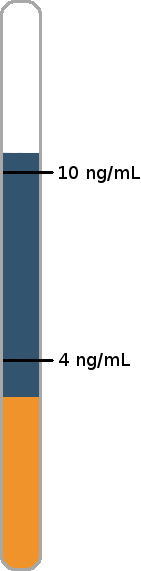
\includegraphics[height=.6\textheight]{./images/screening/high_psa.png}
          \caption{\tiny \tikzbullet{gray}{orangeubfc} free PSA \\ \tikzbullet{gray}{blueubfc} protein-linked PSA}
          \end{figure}
        }
        \only<2>{
          \begin{figure}
          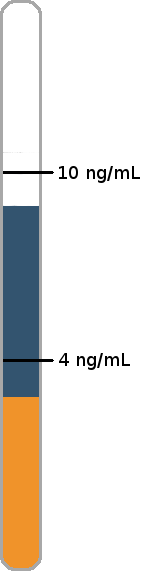
\includegraphics[height=.6\textheight]{./images/screening/risk_psa.png}
          \caption{\tiny \tikzbullet{gray}{orangeubfc} free PSA \\ \tikzbullet{gray}{blueubfc} protein-linked PSA}
          \end{figure}
        }
        \only<3>{
          \begin{figure}
          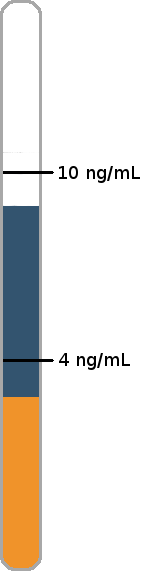
\includegraphics[height=.6\textheight]{./images/screening/risk_psa.png}
          \caption{\tiny \tikzbullet{gray}{orangeubfc} free PSA \\ \tikzbullet{gray}{blueubfc} protein-linked PSA}
          \end{figure}
        }
        \only<4>{
          \begin{figure}
          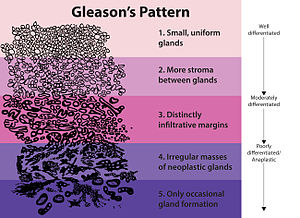
\includegraphics[height=.3\textheight]{./images/screening/gleason.jpg}
          \caption{\tiny Image source: \texttt{https://goo.gl/fEVQXQ}}
          \end{figure}
        }
        \only<5>{
          \begin{figure}
          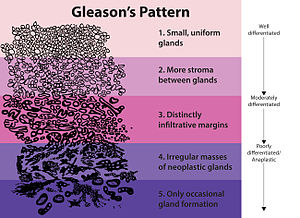
\includegraphics[height=.3\textheight]{./images/screening/gleason.jpg}
          \caption{\tiny Image source: \texttt{https://goo.gl/fEVQXQ}}
          \end{figure}
        }
        \only<6>{
          \begin{greenblock}{\small Pros}
            \begin{itemize}\scriptsize
            \item[\tick]<6-> Reduce CaP-related mortality from \SIrange{21}{44}{\percent}\footnotemark
            \end{itemize}
          \end{greenblock}
          \begin{redblock}{\small Cons}
            \begin{itemize}\scriptsize
            \item[\cross] Up to \SI{30}{\percent} of over-diagnosis\footnotemark
            \item[\cross] Up to \SI{35}{\percent} of undiagnosed CaP\footnotemark
            \item[\cross] Biopsies are invasive
            \end{itemize}
          \end{redblock}}
      \end{center}
    \end{column}
    \only<6>{\addtocounter{footnote}{-3} \stepcounter{footnote} \footcitetext{Schroeder2012} \stepcounter{footnote} \footcitetext{Haas2007} \stepcounter{footnote} \footcitetext{Taira2010}}
  \end{columns}
\end{frame}

\subsection{CAD and mp-MRI}

\begin{frame}
  \frametitle{Introduction}
  \framesubtitle{CAD and mp-MRI}
  \begin{greenblock}{\small Current trendy techniques: mp-MRI}
    \begin{itemize}\scriptsize
    \item[\tick] Less invasive technique
    \end{itemize}
  \end{greenblock}
  \begin{redblock}{\small Human diagnosis using mp-MRI}
    \begin{itemize}\scriptsize
    \item[\cross] Need further investigation of the mp-MRI modalities
    \item[\cross] Low repeatability
      \begin{itemize} \scriptsize
        \item Observer limitations
        \item Complexity of clinical cases
      \end{itemize}
    \end{itemize}
  \end{redblock}
  \begin{block}{\small Emergence of CAD}
    \begin{itemize}\scriptsize
      \item CADe $\rightarrow$ detection of potential lesions
      \item CADx $\rightarrow$ diagnosis regarding those lesions
    \end{itemize}
  \end{block}
\end{frame}

\subsection{Research objectives}

\begin{frame}
  \frametitle{Introduction}
  \framesubtitle{Research objectives}
  \begin{block}{\small Propose a mp-MRI CAD for CaP}
    \begin{itemize}\scriptsize
      \item Study and investigate the state-of-the-art on MRI CAD for CaP
      \item Identify the scientific barriers
      \item Design a mp-MRI CAD addressing these issues
      \item Investigate and analyze the proposed CAD
    \end{itemize}
  \end{block}
\end{frame}

\section{State-of-the-art}

\begin{frame}
    \tableofcontents[currentsection,currentsubsection,subsectionstyle=show/show/hide]
\end{frame}

\subsection{MRI modalities}

\setcounter{subfigure}{0}% Reset subfigure counter

\begin{frame}
  \frametitle{Introduction}
  \framesubtitle{MRI modalities}
  \begin{block}{\small T$_2$W-MRI}
    \begin{figure}%
      \centering
      \hspace*{\fill}%
      \subfigure[][\tiny Healthy]{%
        \label{fig:t2wh}%
        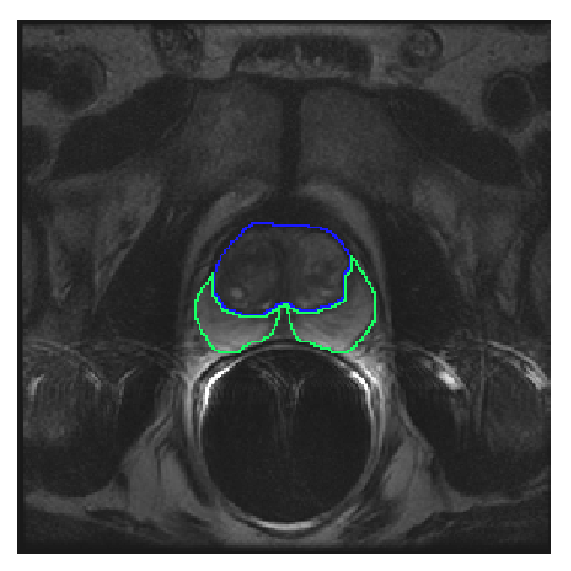
\includegraphics[width=.2\textwidth]{./images/mri/t2w/t2w_healthy.eps}}%
      \hfill%
      \subfigure[][\tiny CaP PZ]{%
        \label{fig:t2wcpz}%
        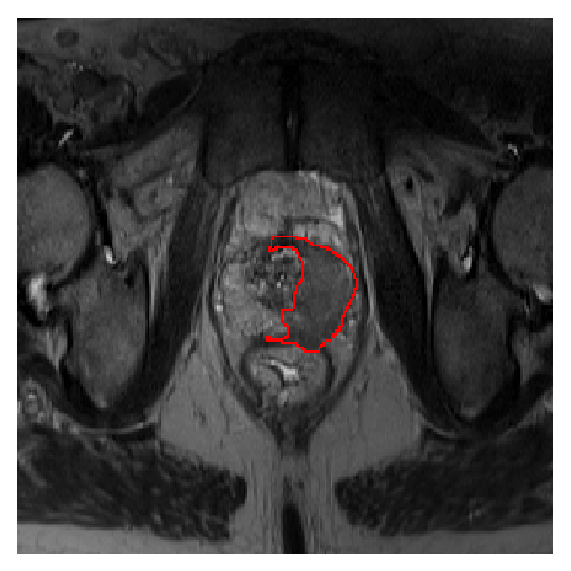
\includegraphics[width=.2\textwidth]{./images/mri/t2w/t2w_cancer_pz.eps}}%
      \hfill%
      \subfigure[][\tiny CaP CG]{%
        \label{fig:t2wccg}%
        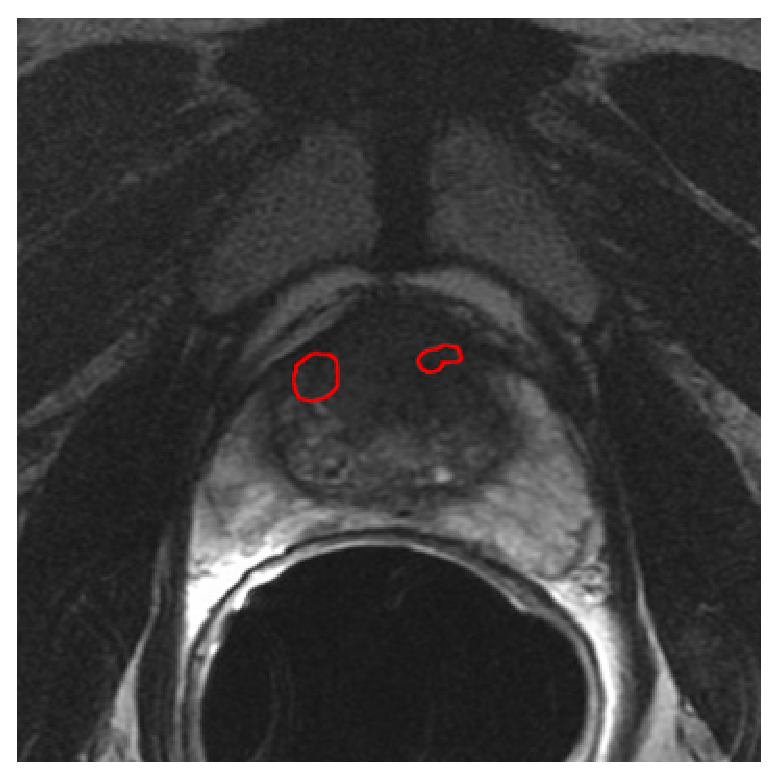
\includegraphics[width=.2\textwidth]{./images/mri/t2w/t2w_cancer_cg.eps}}%
      \hspace*{\fill}%
      \label{fig:t2w}%
    \end{figure}
  \end{block}
  \only<1>{
  \begin{columns}
    \begin{column}{0.5\textwidth}
      \begin{greenblock}{\small Healthy}\footnotesize
        \begin{itemize}\scriptsize
        \item Intermediate to high-signal intensity (SI) in PZ
        \item Low-SI in CG
        \end{itemize}
      \end{greenblock}
    \end{column}
    \begin{column}{0.5\textwidth}
      \begin{redblock}{\small CaP}\footnotesize
        \begin{itemize}\scriptsize
        \item Low-SI
        \item Round and ill-defined mass in PZ
        \item Homogeneous with ill-defined edges in CG
        \end{itemize}
      \end{redblock}
    \end{column}
  \end{columns}}
\only<2>{
  \begin{columns}
    \begin{column}{0.5\textwidth}
      \begin{greenblock}{\small Pros}\footnotesize
        \begin{itemize}\scriptsize
        \item Highest spatial resolution
        \item Anatomy nicely depicted
        \end{itemize}
      \end{greenblock}
    \end{column}
    \begin{column}{0.5\textwidth}
      \begin{redblock}{\small Cons}\footnotesize
        \begin{itemize}\scriptsize
        \item Low sensitivity in CG
        \item Lower specificity due to outliers
        \end{itemize}
      \end{redblock}
    \end{column}
  \end{columns}}
\end{frame}

\setcounter{subfigure}{0}% Reset subfigure counter

\begin{frame}
  \frametitle{Introduction}
  \framesubtitle{MRI modalities}
  \begin{block}{\small DCE-MRI}
    \begin{figure}%
      \centering
      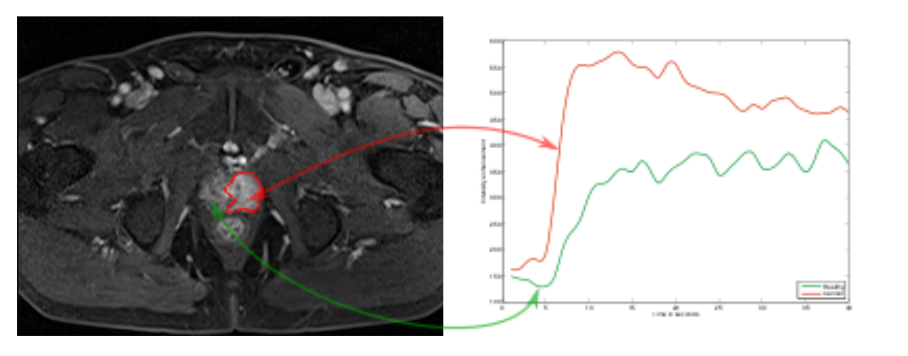
\includegraphics[width=.7\textwidth]{./images/mri/dce/dce_cancer_healthy_information.eps}
      \label{fig:dce}%
      \caption{{\color{green}Green}: healthy - {\color{red}Red}: CaP}
    \end{figure}
  \end{block}
  \only<1>{
  \begin{columns}
    \begin{column}{0.5\textwidth}
      \begin{greenblock}{\small Healthy}
        \begin{itemize}\scriptsize
        \item Slower wash-in, wash-out, time-to-peak enhancement
        \item Lower integral under the curve, max SI
        \end{itemize}
      \end{greenblock}
    \end{column}
    \begin{column}{0.5\textwidth}
      \begin{redblock}{\small CaP}
        \begin{itemize}\scriptsize
        \item Faster wash-in, wash-out, time-to-peak enhancement
        \item Higher integral under the curve, max SI
        \end{itemize}
      \end{redblock}
    \end{column}
  \end{columns}}
\only<2>{
  \begin{columns}
    \begin{column}{0.5\textwidth}
      \begin{greenblock}{\small Pros}\footnotesize
        \begin{itemize}\scriptsize
        \item Information about vascularity
        \end{itemize}
      \end{greenblock}
    \end{column}
    \begin{column}{0.5\textwidth}
      \begin{redblock}{\small Cons}\footnotesize
        \begin{itemize}\scriptsize
        \item Spatial mis-registration
        \item Lower spatial resolution than T$_2$W-MRI
        \item Difficult detection in CG
        \end{itemize}
      \end{redblock}
    \end{column}
  \end{columns}}
\end{frame}

\setcounter{subfigure}{0}% Reset subfigure counter

\begin{frame}
  \frametitle{Introduction}
  \framesubtitle{MRI modalities}
  \begin{block}{\small DW-MRI - ADC}
    \begin{figure}%
      \centering
      \hspace*{\fill}%
      \subfigure[][\tiny DW MRI]{%
        \label{fig:dw}%
        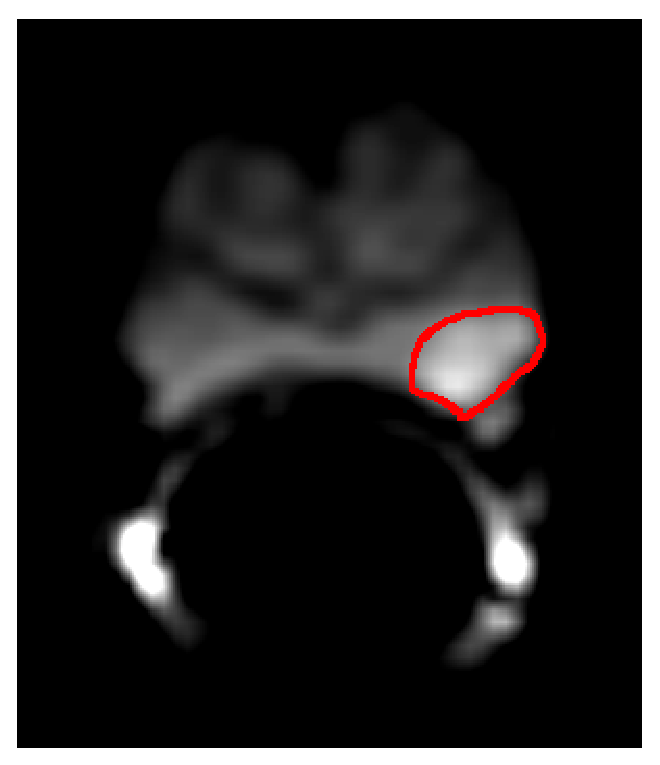
\includegraphics[width=.2\textwidth]{./images/mri/dwi/dwi_cancer.eps}}%
      \hfill%
      \subfigure[][\tiny ADC]{%
        \label{fig:adc}%
        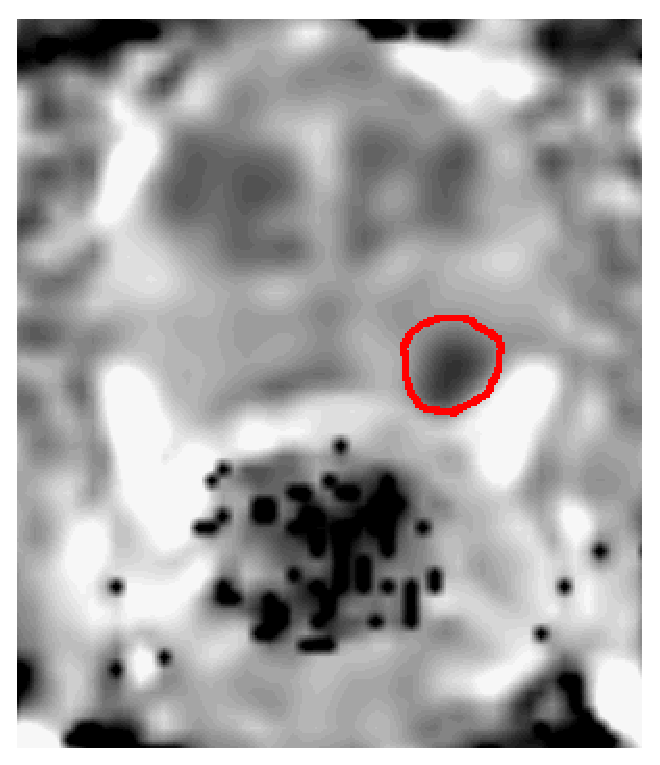
\includegraphics[width=.2\textwidth]{./images/mri/dwi/adc_cancer.eps}}%
      \hspace*{\fill}%
      \label{fig:dwadc}%
    \end{figure}
  \end{block}
  \only<1>{
  \begin{columns}
    \begin{column}{0.5\textwidth}
      \begin{greenblock}{\small Healthy}
        \begin{itemize}\scriptsize
        \item DW-MRI: lower SI
        \item ADC: higher-SI
        \end{itemize}
      \end{greenblock}
    \end{column}
    \begin{column}{0.5\textwidth}
      \begin{redblock}{\small CaP}\scriptsize
        \begin{itemize}
        \item DW-MRI: higher SI
        \item ADC: lower-SI
        \end{itemize}
      \end{redblock}
    \end{column}
  \end{columns}}
  \only<2>{
  \begin{columns}
    \begin{column}{0.5\textwidth}
      \begin{greenblock}{\small Pros}
        \begin{itemize}\scriptsize
        \item Information about tissue structure
        \item ADC correlated with Gleason score
        \end{itemize}
      \end{greenblock}
    \end{column}
    \begin{column}{0.5\textwidth}
      \begin{redblock}{\small Cons}\scriptsize
        \begin{itemize}
        \item Poor spatial resolution
        \item Variability of the ADC coefficient
        \end{itemize}
      \end{redblock}
    \end{column}
  \end{columns}}
\end{frame}

\setcounter{subfigure}{0}% Reset subfigure counter

\begin{frame}
  \frametitle{Introduction}
  \framesubtitle{MRI modalities}
  \begin{block}{\small MRSI}
    \begin{figure}%
      \centering
      \hspace*{\fill}%
      \subfigure[][\tiny Healthy]{%
        \label{fig:mrsih}%
        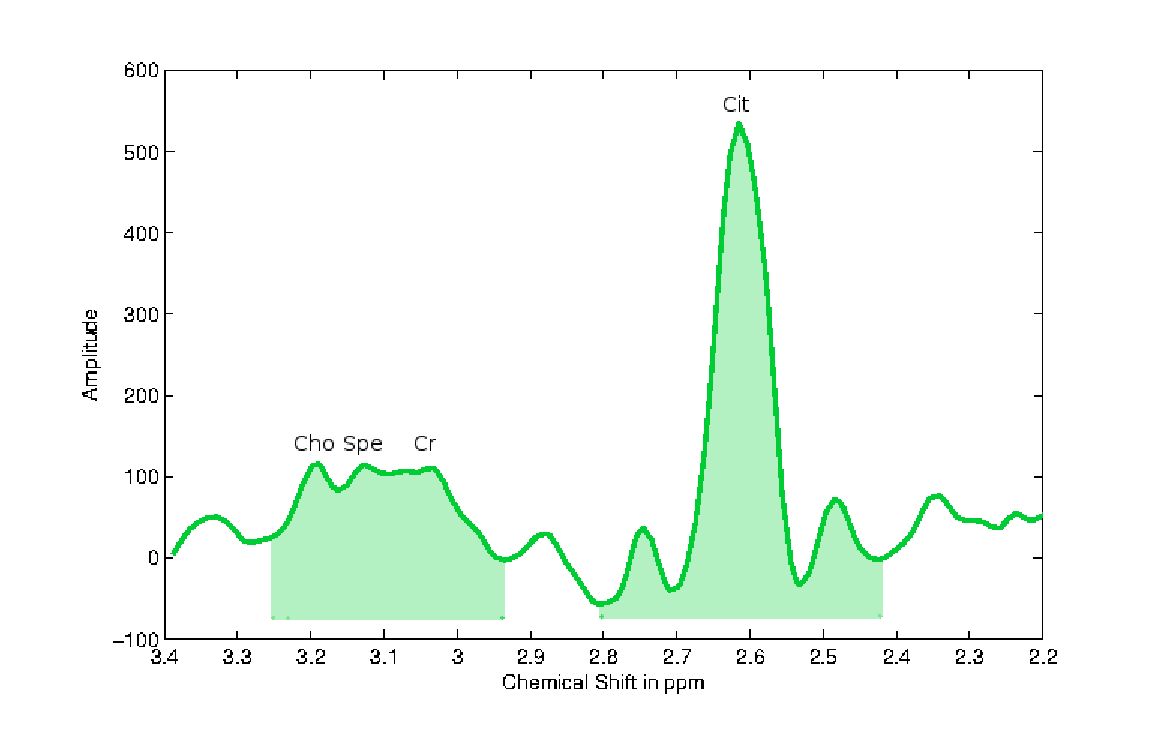
\includegraphics[width=.45\textwidth]{./images/mri/mrsi/mrsi_healthy.eps}}%
      \hfill%
      \subfigure[][\tiny CaP]{%
        \label{fig:mrsic}%
        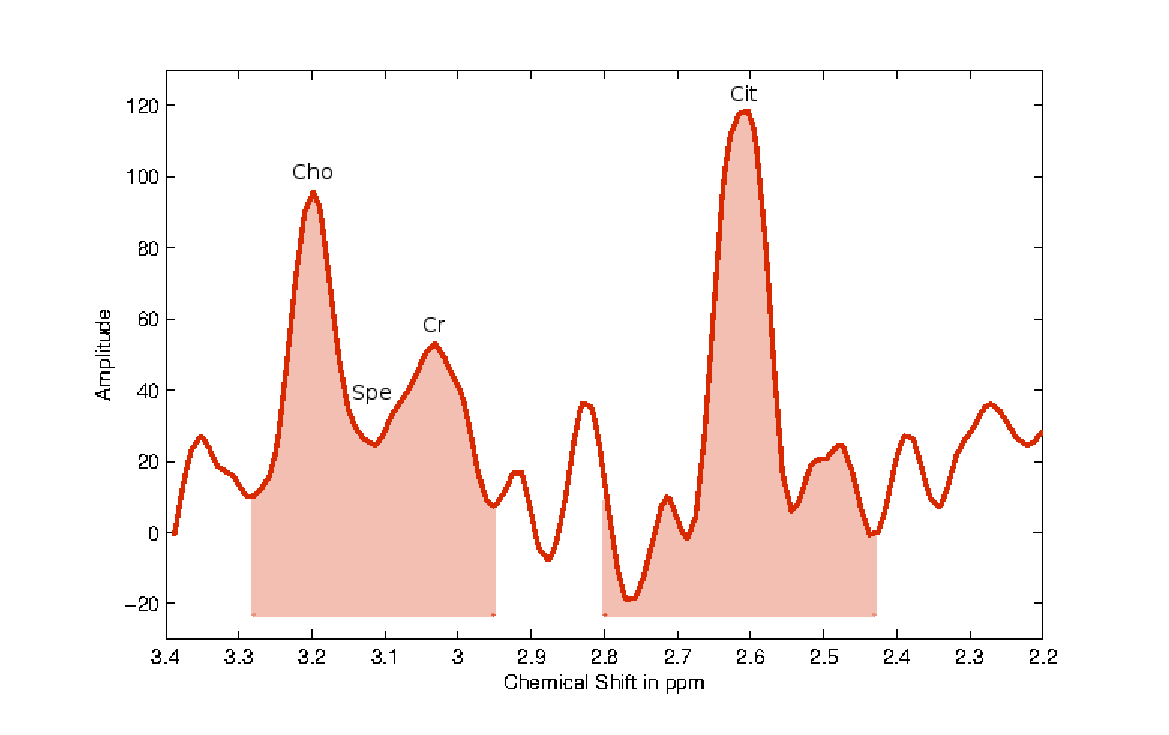
\includegraphics[width=.45\textwidth]{./images/mri/mrsi/mrsi_cancer.eps}}%
      \hspace*{\fill}%
      \label{fig:mrsi}%
    \end{figure}
  \end{block}
  \only<1>{
  \begin{columns}
    \begin{column}{0.5\textwidth}
      \begin{greenblock}{\small Healthy}
        \begin{itemize}\scriptsize
        \item High citrate
        \item Moderate choline and spermine
        \end{itemize}
      \end{greenblock}
    \end{column}
    \begin{column}{0.5\textwidth}
      \begin{redblock}{\small CaP}
        \begin{itemize}\scriptsize
        \item Decrease of citrate and spermine
        \item Increase of choline
        \end{itemize}
      \end{redblock}
    \end{column}
  \end{columns}}
\only<2>{
  \begin{columns}
    \begin{column}{0.5\textwidth}
      \begin{greenblock}{\small Pros}\footnotesize
        \begin{itemize}\scriptsize
        \item Citrate correlated with Gleason score
        \end{itemize}
      \end{greenblock}
    \end{column}
    \begin{column}{0.5\textwidth}
      \begin{redblock}{\small Cons}\footnotesize
        \begin{itemize}\scriptsize
        \item Low spatial resolution
        \item Variation inter-patients
        \end{itemize}
      \end{redblock}
    \end{column}
  \end{columns}}
\end{frame}

\subsection{CAD for CaP}

\begin{frame}
  \frametitle{State-of-the-art}
  \framesubtitle{CAD for CaP}
  \begin{block}{Full CAD for detection and diagnosis of CaP}
  \begin{figure}
  \centering

  % Define block styles used later

  \tikzstyle{module}=[draw, draw=azulunam!80, text width=10em, 
  text centered, minimum height=5em, minimum width = 15em, drop shadow, rounded corners,
  fill=azulunam!30]
  
  \tikzstyle{vecArrow} = [thick, decoration={markings,mark=at position
    1 with {\arrow[semithick]{open triangle 60}}},
  double distance=1.4pt, shorten >= 5.5pt,
  preaction = {decorate},
  postaction = {draw,line width=1.4pt, white,shorten >= 4.5pt}]

  % Define distances for bordering
  \def\blockdist{1.5}
  \def\edgedist{2.5}

  \begin{tikzpicture}[node distance=3cm,thick,scale=0.38, every node/.style={scale=0.38},path image/.style={
      path picture={
        \node at (path picture bounding box.center) {
          \includegraphics[width=1cm]{#1}
        };}}]
    \tikzstyle{conefill} = [path image=,fill opacity=0.8]
    \node[module=above:pre] (pre) at (4.5,-2.6) {\Large Pre-processing};
    \node[module,below of=pre] (seg) {\Large Segmentation};
    \node[module,below of=seg] (reg) {\Large Registration};

    \path[->,dashed] (seg.west) edge [bend right=70] node {} (reg.west);
    \path[->,dashed] (reg.east) edge [bend right=70] node {} (seg.east);

    \draw[->] (pre)--(seg);
    \draw[->] (seg)--(reg);

    \begin{pgfonlayer}{background}
      \path (pre.west |- pre.north)+(-0.9,1.0+\blockdist) node (a) {};
      \path (reg.east |- reg.south)+(+0.9,-0.5) node (b) {};
      
      \path[fill=azulunam!10,rounded corners, draw=azulunam!20, dashed] (a) rectangle (b);
    \end{pgfonlayer}
    
    \path (pre.north) +(0,+\blockdist) node (bgreg) {\Large Image regularization};

    \begin{scope}[node distance=10cm]
      \node[module] (det) [below right=0cm and 3cm of pre] {\Large Features detection};
    \end{scope}
    \begin{scope}[node distance=3.5cm]
      \node[module,above of=det] (roi) {\Large ROIs\\detection/selection};
    \end{scope}
    \node[module,below of=det] (sel) {\Large Features\\selection/extraction};
    \node[module,below of=sel] (cla) {\Large Features\\classification/fusion};

    \draw[->] (roi)--(det);
    \draw[->] (det)--(sel);
    \draw[->] (sel)--(cla);

    \begin{pgfonlayer}{background}
      \path (roi.west |- roi.north)+(-0.25,0.8) node (c) {};
      \path (roi.east |- roi.south)+(+0.25,-0.25) node (d) {};
      
      \path[fill=azulunam!20,rounded corners, draw=azulunam!25, dashed] (c) rectangle (d);
    \end{pgfonlayer}

    \path (roi.west |- roi.north) +(.75,0.4) node (bgfea) {\Large \textbf{CADe}};

    \begin{pgfonlayer}{background}
      \path (det.west |- det.north)+(-0.25,0.8) node (c) {};
      \path (cla.east |- cla.south)+(+0.25,-0.25) node (d) {};
      
      \path[fill=azulunam!20,rounded corners, draw=azulunam!25, dashed] (c) rectangle (d);
    \end{pgfonlayer}

    \path (roi.west |- det.north) +(.75,0.4) node (bgfea) {\Large \textbf{CADx}};     

    % Define the place where the arrow should start anf finish
    \path (seg.east |- seg.north)+(+1.15,0) node (e) {};
    \path (sel.west |- seg.north)+(-1.0,0) node (f) {};

    \draw[double distance =3pt,preaction={-triangle 90,thin,draw,shorten >=-1mm}] (e) -- (f) node[midway,above,above=1em] {\Large Regularized data};

    \begin{scope}[yshift=34,xshift=-86]
      \transparent{0.6}\draw[path image=images/tikzimage/t2.eps] (0,0) rectangle (1.0,1.0);
    \end{scope}

    \begin{scope}[yshift=31,xshift=-83]
      \transparent{0.6}\draw[path image=images/tikzimage/t2.eps] (0,0) rectangle (1.0,1.0);
    \end{scope}

    \begin{scope}[yshift=28,xshift=-80]
      \transparent{0.8}\draw[path image=images/tikzimage/t2.eps] (0,0) rectangle (1.0,1.0);
      \path (0,0)+(-1.65,0.3) node {\Large T$_2$-W MRI};
    \end{scope}

    \begin{scope}[yshift=-33,xshift=-86]
      \transparent{0.6}\draw[path image=images/tikzimage/t2.eps] (0,0) rectangle (1.0,1.0);
    \end{scope}

    \begin{scope}[yshift=-36,xshift=-83]
      \transparent{0.6}\draw[path image=images/tikzimage/t2.eps] (0,0) rectangle (1.0,1.0);
    \end{scope}

    \begin{scope}[yshift=-39,xshift=-80]
      \transparent{0.8}\draw[path image=images/tikzimage/t2.eps] (0,0) rectangle (1.0,1.0);
      \path (0,0)+(-1.35,0.3) node {\Large T$_2$ map};
    \end{scope}

    \begin{scope}[yshift=-100,xshift=-86]
      \transparent{0.6}\draw[path image=images/tikzimage/dce.eps] (0,0) rectangle (1.0,1.0);
    \end{scope}

    \begin{scope}[yshift=-103,xshift=-83]
      \transparent{0.6}\draw[path image=images/tikzimage/dce.eps] (0,0) rectangle (1.0,1.0);
    \end{scope}

    \begin{scope}[yshift=-106,xshift=-80]
      \transparent{0.8}\draw[path image=images/tikzimage/dce.eps] (0,0) rectangle (1.0,1.0);
      \path (0,0)+(-1.65,0.3) node {\Large DCE-MRI};
    \end{scope}

    \begin{scope}[yshift=-167,xshift=-86]
      \transparent{0.6}\draw[path image=images/tikzimage/dwi1.eps] (0,0) rectangle (1.0,1.0);
    \end{scope}

    \begin{scope}[yshift=-170,xshift=-83]
      \transparent{0.6}\draw[path image=images/tikzimage/dwi1.eps] (0,0) rectangle (1.0,1.0);
    \end{scope}

    \begin{scope}[yshift=-173,xshift=-80]
      \transparent{0.8}\draw[path image=images/tikzimage/dwi1.eps] (0,0) rectangle (1.0,1.0);
      \path (0,0)+(-1.65,0.3) node {\Large DW-MRI};
    \end{scope}

    \begin{scope}[yshift=-234,xshift=-86]
      \transparent{0.6}\draw[path image=images/tikzimage/dwi1.eps] (0,0) rectangle (1.0,1.0);
    \end{scope}

    \begin{scope}[yshift=-237,xshift=-83]
      \transparent{0.6}\draw[path image=images/tikzimage/dwi1.eps] (0,0) rectangle (1.0,1.0);
    \end{scope}

    \begin{scope}[yshift=-240,xshift=-80]
      \transparent{0.8}\draw[path image=images/tikzimage/dwi1.eps] (0,0) rectangle (1.0,1.0);
      \path (0,0)+(-1.5,0.3) node {\Large ADC};
    \end{scope}

    \begin{scope}[yshift=-301,xshift=-86]
      \transparent{0.6}\draw[path image=images/tikzimage/mrsi.eps] (0,0) rectangle (1.0,1.0);
    \end{scope}

    \begin{scope}[yshift=-304,xshift=-83]
      \transparent{0.6}\draw[path image=images/tikzimage/mrsi.eps] (0,0) rectangle (1.0,1.0);
    \end{scope}

    \begin{scope}[yshift=-307,xshift=-80]
      \transparent{0.8}\draw[path image=images/tikzimage/mrsi.eps] (0,0) rectangle (1.0,1.0);
      \path (0,0)+(-1.1,0.3) node {\Large MRSI};
    \end{scope}

    \path (pre.west |- roi.north)+(-3.5,1.0+\blockdist) node (g) {};
    \path (reg.west |- cla.south)+(-3.5,-0.5) node (h) {};

    \draw[decorate,decoration={brace,raise=6pt,amplitude=10pt}, thick]
    (g)--(h) ;
    
    \path (seg.west |- seg.north)+(-2.5,0) node (i) {};
    \path (seg.west |- seg.north)+(-0.9,0) node (j) {};
    
    % \draw[double distance =3pt,preaction={-triangle 90,thin,draw,shorten >=-1mm}] (i) -- (j);   

    \path (sel.east |- seg.north)+(2,0) node (k) {};
    \path (sel.east |- seg.north)+(0.5,0) node (l) {};
    
  \end{tikzpicture}
  \caption{Common CAD framework based on MRI images used to detect CaP}
  \label{fig:wkfcad}
\end{figure}

  \end{block}
\end{frame}

\begin{frame}
  \frametitle{State-of-the-art}
  \framesubtitle{CAD for CaP}
  \begin{columns}
    \begin{column}{0.5\textwidth}
      \only<1>{
      \begin{greenblock}{\small Conclusions}
        \begin{itemize}\scriptsize
          \item[\tick]<1-> 3 modalities better than 2
          \item[\tick]<2-> Texture and edge features are predominant
          \item[\tick]<3-> Feature selection/extraction tends to improve performance
          \item[\tick]<4-> Pre-eminence of SVM and ensemble classifier (i.e., AdaBoost, RF, etc.)
        \end{itemize}
      \end{greenblock}}
      \only<2>{
      \begin{greenblock}{\small Conclusions}
        \begin{itemize}\scriptsize
          \item[\tick]<1-> 3 modalities better than 2
          \item[\tick]<2-> Texture and edge features are predominant
          \item[\tick]<3-> Feature selection/extraction tends to improve performance
          \item[\tick]<4-> Pre-eminence of SVM and ensemble classifier (i.e., AdaBoost, RF, etc.)
        \end{itemize}
      \end{greenblock}}
      \only<3>{
      \begin{greenblock}{\small Conclusions}
        \begin{itemize}\scriptsize
          \item[\tick]<1-> 3 modalities better than 2
          \item[\tick]<2-> Texture and edge features are predominant
          \item[\tick]<3-> Feature selection/extraction tends to improve performance
          \item[\tick]<4-> Pre-eminence of SVM and ensemble classifier (i.e., AdaBoost, RF, etc.)
        \end{itemize}
      \end{greenblock}}
      \only<4>{
      \begin{greenblock}{\small Conclusions}
        \begin{itemize}\scriptsize
          \item[\tick]<1-> 3 modalities better than 2
          \item[\tick]<2-> Texture and edge features are predominant
          \item[\tick]<3-> Feature selection/extraction tends to improve performance
          \item[\tick]<4-> Pre-eminence of SVM and ensemble classifier (i.e., AdaBoost, RF, etc.)
        \end{itemize}
      \end{greenblock}}
      \only<5>{
      \begin{greenblock}{\small Conclusions}
        \begin{itemize}\scriptsize
          \item[\tick]<1-> 3 modalities better than 2
          \item[\tick]<2-> Texture and edge features are predominant
          \item[\tick]<3-> Feature selection/extraction tends to improve performance
          \item[\tick]<4-> Pre-eminence of SVM and ensemble classifier (i.e., AdaBoost, RF, etc.)
        \end{itemize}
      \end{greenblock}}
      \only<6>{
          \begin{figure}
  \centering

  % Define block styles used later

  \tikzstyle{module}=[draw, draw=blue!80, text width=10em, 
  text centered, minimum height=5em, minimum width = 15em, drop shadow, rounded corners,
  fill=blue!30]
  
  \tikzstyle{vecArrow} = [thick, decoration={markings,mark=at position
    1 with {\arrow[semithick]{open triangle 60}}},
  double distance=1.4pt, shorten >= 5.5pt,
  preaction = {decorate},
  postaction = {draw,line width=1.4pt, white,shorten >= 4.5pt}]

  % Define distances for bordering
  \def\blockdist{1.5}
  \def\edgedist{2.5}

  \begin{tikzpicture}[node distance=3cm,thick,scale=0.2, every node/.style={scale=0.2},path image/.style={
      path picture={
        \node at (path picture bounding box.center) {
          \includegraphics[width=1cm]{#1}
        };}}]
    \tikzstyle{conefill} = [path image=,fill opacity=0.8]
    \node[module=above:pre] (pre) at (4.5,-2.6) {\Large Pre-processing};
    \node[module,below of=pre] (seg) {\Large Segmentation};
    \node[module,below of=seg] (reg) {\Large Registration};

    \path[->,dashed] (seg.west) edge [bend right=70] node {} (reg.west);
    \path[->,dashed] (reg.east) edge [bend right=70] node {} (seg.east);

    \draw[->] (pre)--(seg);
    \draw[->] (seg)--(reg);

    \begin{pgfonlayer}{background}
      \path (pre.west |- pre.north)+(-0.9,1.0+\blockdist) node (a) {};
      \path (reg.east |- reg.south)+(+0.9,-0.5) node (b) {};
      
      \path[fill=blue!10,rounded corners, draw=blue!20, dashed] (a) rectangle (b);
    \end{pgfonlayer}
    
    \path (pre.north) +(0,+\blockdist) node (bgreg) {\Large Image regularization};

    \begin{scope}[node distance=10cm]
      \node[module] (det) [below right=0cm and 1cm of pre] {\Large Features detection};
    \end{scope}
    \begin{scope}[node distance=3.5cm]
      \node[module,above of=det] (roi) {\Large ROIs\\detection/selection};
    \end{scope}
    \node[module,below of=det] (sel) {\Large Features\\selection/extraction};
    \node[module,below of=sel] (cla) {\Large Features\\classification/fusion};

    \draw[->] (roi)--(det);
    \draw[->] (det)--(sel);
    \draw[->] (sel)--(cla);

    \begin{pgfonlayer}{background}
      \path (roi.west |- roi.north)+(-0.25,0.8) node (c) {};
      \path (roi.east |- roi.south)+(+0.25,-0.25) node (d) {};
      
      \path[fill=blue!20,rounded corners, draw=blue!25, dashed] (c) rectangle (d);
    \end{pgfonlayer}

    \path (roi.west |- roi.north) +(.75,0.4) node (bgfea) {\Large \textbf{CADe}};

    \begin{pgfonlayer}{background}
      \path (det.west |- det.north)+(-0.25,0.8) node (c) {};
      \path (cla.east |- cla.south)+(+0.25,-0.25) node (d) {};
      
      \path[fill=blue!20,rounded corners, draw=blue!25, dashed] (c) rectangle (d);
    \end{pgfonlayer}

    \path (roi.west |- det.north) +(.75,0.4) node (bgfea) {\Large \textbf{CADx}};     

    \begin{pgfonlayer}{background}
      \filldraw[fill=red!20!white,rounded corners,draw=red!25,dashed] (-6,3) rectangle (0,-12);
    \end{pgfonlayer}

    % Define the place where the arrow should start anf finish
    \path (seg.east |- seg.north)+(+1.15,0) node (e) {};
    \path (sel.west |- seg.north)+(-1.0,0) node (f) {};

    \draw[double distance =3pt,preaction={-triangle 90,thin,draw,shorten >=-1mm}] (e) -- (f) node[midway,above,above=.3em] {\large Regularized data};

    \begin{scope}[yshift=34,xshift=-86]
      \transparent{0.6}\draw[path image=images/tikzimage/t2.eps] (0,0) rectangle (1.0,1.0);
    \end{scope}

    \begin{scope}[yshift=31,xshift=-83]
      \transparent{0.6}\draw[path image=images/tikzimage/t2.eps] (0,0) rectangle (1.0,1.0);
    \end{scope}

    \begin{scope}[yshift=28,xshift=-80]
      \transparent{0.8}\draw[path image=images/tikzimage/t2.eps] (0,0) rectangle (1.0,1.0);
      \path (0,0)+(-1.65,0.3) node {\Large T$_2$-W MRI};
    \end{scope}

    \begin{scope}[yshift=-33,xshift=-86]
      \transparent{0.6}\draw[path image=images/tikzimage/t2.eps] (0,0) rectangle (1.0,1.0);
    \end{scope}

    \begin{scope}[yshift=-36,xshift=-83]
      \transparent{0.6}\draw[path image=images/tikzimage/t2.eps] (0,0) rectangle (1.0,1.0);
    \end{scope}

    \begin{scope}[yshift=-39,xshift=-80]
      \transparent{0.8}\draw[path image=images/tikzimage/t2.eps] (0,0) rectangle (1.0,1.0);
      \path (0,0)+(-1.35,0.3) node {\Large T$_2$ map};
    \end{scope}

    \begin{scope}[yshift=-100,xshift=-86]
      \transparent{0.6}\draw[path image=images/tikzimage/dce.eps] (0,0) rectangle (1.0,1.0);
    \end{scope}

    \begin{scope}[yshift=-103,xshift=-83]
      \transparent{0.6}\draw[path image=images/tikzimage/dce.eps] (0,0) rectangle (1.0,1.0);
    \end{scope}

    \begin{scope}[yshift=-106,xshift=-80]
      \transparent{0.8}\draw[path image=images/tikzimage/dce.eps] (0,0) rectangle (1.0,1.0);
      \path (0,0)+(-1.65,0.3) node {\Large DCE-MRI};
    \end{scope}

    \begin{scope}[yshift=-167,xshift=-86]
      \transparent{0.6}\draw[path image=images/tikzimage/dwi1.eps] (0,0) rectangle (1.0,1.0);
    \end{scope}

    \begin{scope}[yshift=-170,xshift=-83]
      \transparent{0.6}\draw[path image=images/tikzimage/dwi1.eps] (0,0) rectangle (1.0,1.0);
    \end{scope}

    \begin{scope}[yshift=-173,xshift=-80]
      \transparent{0.8}\draw[path image=images/tikzimage/dwi1.eps] (0,0) rectangle (1.0,1.0);
      \path (0,0)+(-1.65,0.3) node {\Large DW-MRI};
    \end{scope}

    \begin{scope}[yshift=-234,xshift=-86]
      \transparent{0.6}\draw[path image=images/tikzimage/dwi1.eps] (0,0) rectangle (1.0,1.0);
    \end{scope}

    \begin{scope}[yshift=-237,xshift=-83]
      \transparent{0.6}\draw[path image=images/tikzimage/dwi1.eps] (0,0) rectangle (1.0,1.0);
    \end{scope}

    \begin{scope}[yshift=-240,xshift=-80]
      \transparent{0.8}\draw[path image=images/tikzimage/dwi1.eps] (0,0) rectangle (1.0,1.0);
      \path (0,0)+(-1.5,0.3) node {\Large ADC};
    \end{scope}

    \begin{scope}[yshift=-301,xshift=-86]
      \transparent{0.6}\draw[path image=images/tikzimage/mrsi.eps] (0,0) rectangle (1.0,1.0);
    \end{scope}

    \begin{scope}[yshift=-304,xshift=-83]
      \transparent{0.6}\draw[path image=images/tikzimage/mrsi.eps] (0,0) rectangle (1.0,1.0);
    \end{scope}

    \begin{scope}[yshift=-307,xshift=-80]
      \transparent{0.8}\draw[path image=images/tikzimage/mrsi.eps] (0,0) rectangle (1.0,1.0);
      \path (0,0)+(-1.1,0.3) node {\Large MRSI};
    \end{scope}

    \path (pre.west |- roi.north)+(-3.5,1.0+\blockdist) node (g) {};
    \path (reg.west |- cla.south)+(-3.5,-0.5) node (h) {};

    \draw[decorate,decoration={brace,raise=2pt,amplitude=5pt}, thick]
    (g)--(h) ;
    
    \path (seg.west |- seg.north)+(-2.5,0) node (i) {};
    \path (seg.west |- seg.north)+(-0.9,0) node (j) {};
    
    % \draw[double distance =3pt,preaction={-triangle 90,thin,draw,shorten >=-1mm}] (i) -- (j);   

    \path (sel.east |- seg.north)+(2,0) node (k) {};
    \path (sel.east |- seg.north)+(0.5,0) node (l) {};
    
  \end{tikzpicture}
\end{figure}

      }
      \only<7>{
          \begin{figure}
  \centering

  % Define block styles used later

  \tikzstyle{module}=[draw, draw=azulunam!80, text width=15em, 
  text centered, minimum height=5em, minimum width = 15em, drop shadow, rounded corners,
  fill=azulunam!30]
  \tikzstyle{modulegreen}=[draw, draw=green!80, text width=15em, 
  text centered, minimum height=5em, minimum width = 15em, drop shadow, rounded corners,
  fill=green!30]
  \tikzstyle{modulered}=[draw, draw=red!80, text width=15em, 
  text centered, minimum height=5em, minimum width = 15em, drop shadow, rounded corners,
  fill=red!30]
  
  \tikzstyle{vecArrow} = [thick, decoration={markings,mark=at position
    1 with {\arrow[semithick]{open triangle 60}}},
  double distance=1.4pt, shorten >= 5.5pt,
  preaction = {decorate},
  postaction = {draw,line width=1.4pt, white,shorten >= 4.5pt}]

  % Define distances for bordering
  \def\blockdist{1.5}
  \def\edgedist{2.5}

  \begin{tikzpicture}[node distance=3cm,thick,scale=0.2, every node/.style={scale=0.2},path image/.style={
      path picture={
        \node at (path picture bounding box.center) {
          \includegraphics[width=1cm]{#1}
        };}}]
    \tikzstyle{conefill} = [path image=,fill opacity=0.8]
    \node[modulered=above:pre] (pre) at (4.5,-2.6) {\Large \textbf{Pre-processing}};
    \node[module,below of=pre] (seg) {\Large \textbf{Segmentation}};
    \node[module,below of=seg] (reg) {\Large \textbf{Registration}};

    \path[->,dashed] (seg.west) edge [bend right=70] node {} (reg.west);
    \path[->,dashed] (reg.east) edge [bend right=70] node {} (seg.east);

    \draw[->] (pre)--(seg);
    \draw[->] (seg)--(reg);

    \begin{pgfonlayer}{background}
      \path (pre.west |- pre.north)+(-0.9,1.0+\blockdist) node (a) {};
      \path (reg.east |- reg.south)+(+0.9,-0.5) node (b) {};
      
      \path[fill=azulunam!10,rounded corners, draw=azulunam!20, dashed] (a) rectangle (b);
    \end{pgfonlayer}
    
    \path (pre.north) +(0,+\blockdist) node (bgreg) {\Large \textbf{Image regularization}};

    \begin{scope}[node distance=10cm]
      \node[module] (det) [below right=0cm and 1cm of pre] {\Large \textbf{Features detection}};
    \end{scope}
    \begin{scope}[node distance=3.5cm]
      \node[module,above of=det] (roi) {\Large \textbf{ROIs\\detection/selection}};
    \end{scope}
    \node[module,below of=det] (sel) {\Large \textbf{Features\\selection/extraction}};
    \node[module,below of=sel] (cla) {\Large \textbf{Features\\classification}};

    \draw[->] (roi)--(det);
    \draw[->] (det)--(sel);
    \draw[->] (sel)--(cla);

    \begin{pgfonlayer}{background}
      \path (roi.west |- roi.north)+(-0.25,0.8) node (c) {};
      \path (roi.east |- roi.south)+(+0.25,-0.25) node (d) {};
      
      \path[fill=azulunam!20,rounded corners, draw=azulunam!25, dashed] (c) rectangle (d);
    \end{pgfonlayer}

    \path (roi.west |- roi.north) +(.75,0.4) node (bgfea) {\Large \textbf{CADe}};

    \begin{pgfonlayer}{background}
      \path (det.west |- det.north)+(-0.25,0.8) node (c) {};
      \path (cla.east |- cla.south)+(+0.25,-0.25) node (d) {};
      
      \path[fill=azulunam!20,rounded corners, draw=azulunam!25, dashed] (c) rectangle (d);
    \end{pgfonlayer}

    \path (roi.west |- det.north) +(.75,0.4) node (bgfea) {\Large \textbf{CADx}};     

    % \begin{scope}
    %   \transparent{0.6}\filldraw[fill=red!20!white,rounded corners,draw=red!25,dashed] (1,-1.1) rectangle (8,-4.1);
    % \end{scope}

    % Define the place where the arrow should start anf finish
    \path (seg.east |- seg.north)+(+1.15,0) node (e) {};
    \path (sel.west |- seg.north)+(-1.0,0) node (f) {};

    \draw[double distance =3pt,preaction={-triangle 90,thin,draw,shorten >=-1mm}] (e) -- (f) node[midway,above,above=.3em] {\large \textbf{Regularized data}};

    \begin{scope}[yshift=34,xshift=-86]
      \transparent{0.6}\draw[path image=images/tikzimage/t2.eps] (0,0) rectangle (1.0,1.0);
    \end{scope}

    \begin{scope}[yshift=31,xshift=-83]
      \transparent{0.6}\draw[path image=images/tikzimage/t2.eps] (0,0) rectangle (1.0,1.0);
    \end{scope}

    \begin{scope}[yshift=28,xshift=-80]
      \transparent{0.8}\draw[path image=images/tikzimage/t2.eps] (0,0) rectangle (1.0,1.0);
      \path (0,0)+(-1.65,0.3) node {\Large \textbf{T$_2$-W MRI}};
    \end{scope}

    \begin{scope}[yshift=-33,xshift=-86]
      \transparent{0.6}\draw[path image=images/tikzimage/t2.eps] (0,0) rectangle (1.0,1.0);
    \end{scope}

    \begin{scope}[yshift=-36,xshift=-83]
      \transparent{0.6}\draw[path image=images/tikzimage/t2.eps] (0,0) rectangle (1.0,1.0);
    \end{scope}

    \begin{scope}[yshift=-39,xshift=-80]
      \transparent{0.8}\draw[path image=images/tikzimage/t2.eps] (0,0) rectangle (1.0,1.0);
      \path (0,0)+(-1.35,0.3) node {\Large \textbf{T$_2$ map}};
    \end{scope}

    \begin{scope}[yshift=-100,xshift=-86]
      \transparent{0.6}\draw[path image=images/tikzimage/dce.eps] (0,0) rectangle (1.0,1.0);
    \end{scope}

    \begin{scope}[yshift=-103,xshift=-83]
      \transparent{0.6}\draw[path image=images/tikzimage/dce.eps] (0,0) rectangle (1.0,1.0);
    \end{scope}

    \begin{scope}[yshift=-106,xshift=-80]
      \transparent{0.8}\draw[path image=images/tikzimage/dce.eps] (0,0) rectangle (1.0,1.0);
      \path (0,0)+(-1.65,0.3) node {\Large \textbf{DCE-MRI}};
    \end{scope}

    \begin{scope}[yshift=-167,xshift=-86]
      \transparent{0.6}\draw[path image=images/tikzimage/dwi1.eps] (0,0) rectangle (1.0,1.0);
    \end{scope}

    \begin{scope}[yshift=-170,xshift=-83]
      \transparent{0.6}\draw[path image=images/tikzimage/dwi1.eps] (0,0) rectangle (1.0,1.0);
    \end{scope}

    \begin{scope}[yshift=-173,xshift=-80]
      \transparent{0.8}\draw[path image=images/tikzimage/dwi1.eps] (0,0) rectangle (1.0,1.0);
      \path (0,0)+(-1.65,0.3) node {\Large \textbf{DW-MRI}};
    \end{scope}

    \begin{scope}[yshift=-234,xshift=-86]
      \transparent{0.6}\draw[path image=images/tikzimage/dwi1.eps] (0,0) rectangle (1.0,1.0);
    \end{scope}

    \begin{scope}[yshift=-237,xshift=-83]
      \transparent{0.6}\draw[path image=images/tikzimage/dwi1.eps] (0,0) rectangle (1.0,1.0);
    \end{scope}

    \begin{scope}[yshift=-240,xshift=-80]
      \transparent{0.8}\draw[path image=images/tikzimage/dwi1.eps] (0,0) rectangle (1.0,1.0);
      \path (0,0)+(-1.5,0.3) node {\Large \textbf{ADC}};
    \end{scope}

    \begin{scope}[yshift=-301,xshift=-86]
      \transparent{0.6}\draw[path image=images/tikzimage/mrsi.eps] (0,0) rectangle (1.0,1.0);
    \end{scope}

    \begin{scope}[yshift=-304,xshift=-83]
      \transparent{0.6}\draw[path image=images/tikzimage/mrsi.eps] (0,0) rectangle (1.0,1.0);
    \end{scope}

    \begin{scope}[yshift=-307,xshift=-80]
      \transparent{0.8}\draw[path image=images/tikzimage/mrsi.eps] (0,0) rectangle (1.0,1.0);
      \path (0,0)+(-1.1,0.3) node {\Large \textbf{MRSI}};
    \end{scope}

    \path (pre.west |- roi.north)+(-3.5,1.0+\blockdist) node (g) {};
    \path (reg.west |- cla.south)+(-3.5,-0.5) node (h) {};

    \draw[decorate,decoration={brace,raise=2pt,amplitude=5pt}, thick]
    (g)--(h) ;
    
    \path (seg.west |- seg.north)+(-2.5,0) node (i) {};
    \path (seg.west |- seg.north)+(-0.9,0) node (j) {};
    
    % \draw[double distance =3pt,preaction={-triangle 90,thin,draw,shorten >=-1mm}] (i) -- (j);   

    \path (sel.east |- seg.north)+(2,0) node (k) {};
    \path (sel.east |- seg.north)+(0.5,0) node (l) {};
    
  \end{tikzpicture}
\end{figure}

      }
      \only<8>{
          \begin{figure}
  \centering

  % Define block styles used later

  \tikzstyle{module}=[draw, draw=azulunam!80, text width=15em, 
  text centered, minimum height=5em, minimum width = 15em, drop shadow, rounded corners,
  fill=azulunam!30]
  \tikzstyle{modulegreen}=[draw, draw=green!80, text width=15em, 
  text centered, minimum height=5em, minimum width = 15em, drop shadow, rounded corners,
  fill=green!30]
  \tikzstyle{modulered}=[draw, draw=red!80, text width=15em, 
  text centered, minimum height=5em, minimum width = 15em, drop shadow, rounded corners,
  fill=red!30]
  
  \tikzstyle{vecArrow} = [thick, decoration={markings,mark=at position
    1 with {\arrow[semithick]{open triangle 60}}},
  double distance=1.4pt, shorten >= 5.5pt,
  preaction = {decorate},
  postaction = {draw,line width=1.4pt, white,shorten >= 4.5pt}]

  % Define distances for bordering
  \def\blockdist{1.5}
  \def\edgedist{2.5}

  \begin{tikzpicture}[node distance=3cm,thick,scale=0.2, every node/.style={scale=0.2},path image/.style={
      path picture={
        \node at (path picture bounding box.center) {
          \includegraphics[width=1cm]{#1}
        };}}]
    \tikzstyle{conefill} = [path image=,fill opacity=0.8]
    \node[module=above:pre] (pre) at (4.5,-2.6) {\Large \textbf{Pre-processing}};
    \node[module,below of=pre] (seg) {\Large \textbf{Segmentation}};
    \node[module,below of=seg] (reg) {\Large \textbf{Registration}};

    \path[->,dashed] (seg.west) edge [bend right=70] node {} (reg.west);
    \path[->,dashed] (reg.east) edge [bend right=70] node {} (seg.east);

    \draw[->] (pre)--(seg);
    \draw[->] (seg)--(reg);

    \begin{pgfonlayer}{background}
      \path (pre.west |- pre.north)+(-0.9,1.0+\blockdist) node (a) {};
      \path (reg.east |- reg.south)+(+0.9,-0.5) node (b) {};
      
      \path[fill=azulunam!10,rounded corners, draw=azulunam!20, dashed] (a) rectangle (b);
    \end{pgfonlayer}
    
    \path (pre.north) +(0,+\blockdist) node (bgreg) {\Large \textbf{Image regularization}};

    \begin{scope}[node distance=10cm]
      \node[modulered] (det) [below right=0cm and 1cm of pre] {\Large \textbf{Features detection}};
    \end{scope}
    \begin{scope}[node distance=3.5cm]
      \node[module,above of=det] (roi) {\Large \textbf{ROIs\\detection/selection}};
    \end{scope}
    \node[module,below of=det] (sel) {\Large \textbf{Features\\selection/extraction}};
    \node[module,below of=sel] (cla) {\Large \textbf{Features\\classification}};

    \draw[->] (roi)--(det);
    \draw[->] (det)--(sel);
    \draw[->] (sel)--(cla);

    \begin{pgfonlayer}{background}
      \path (roi.west |- roi.north)+(-0.25,0.8) node (c) {};
      \path (roi.east |- roi.south)+(+0.25,-0.25) node (d) {};
      
      \path[fill=azulunam!20,rounded corners, draw=azulunam!25, dashed] (c) rectangle (d);
    \end{pgfonlayer}

    \path (roi.west |- roi.north) +(.75,0.4) node (bgfea) {\Large \textbf{CADe}};

    \begin{pgfonlayer}{background}
      \path (det.west |- det.north)+(-0.25,0.8) node (c) {};
      \path (cla.east |- cla.south)+(+0.25,-0.25) node (d) {};
      
      \path[fill=azulunam!20,rounded corners, draw=azulunam!25, dashed] (c) rectangle (d);
    \end{pgfonlayer}

    \path (roi.west |- det.north) +(.75,0.4) node (bgfea) {\Large \textbf{CADx}};     

    % \begin{scope}
    %   \transparent{0.6}\filldraw[fill=red!20!white,rounded corners,draw=red!25,dashed] (11.5,-3) rectangle (19,-6);
    % \end{scope}

    % Define the place where the arrow should start anf finish
    \path (seg.east |- seg.north)+(+1.15,0) node (e) {};
    \path (sel.west |- seg.north)+(-1.0,0) node (f) {};

    \draw[double distance =3pt,preaction={-triangle 90,thin,draw,shorten >=-1mm}] (e) -- (f) node[midway,above,above=.3em] {\large \textbf{Regularized data}};

    \begin{scope}[yshift=34,xshift=-86]
      \transparent{0.6}\draw[path image=images/tikzimage/t2.eps] (0,0) rectangle (1.0,1.0);
    \end{scope}

    \begin{scope}[yshift=31,xshift=-83]
      \transparent{0.6}\draw[path image=images/tikzimage/t2.eps] (0,0) rectangle (1.0,1.0);
    \end{scope}

    \begin{scope}[yshift=28,xshift=-80]
      \transparent{0.8}\draw[path image=images/tikzimage/t2.eps] (0,0) rectangle (1.0,1.0);
      \path (0,0)+(-1.65,0.3) node {\Large \textbf{T$_2$-W MRI}};
    \end{scope}

    \begin{scope}[yshift=-33,xshift=-86]
      \transparent{0.6}\draw[path image=images/tikzimage/t2.eps] (0,0) rectangle (1.0,1.0);
    \end{scope}

    \begin{scope}[yshift=-36,xshift=-83]
      \transparent{0.6}\draw[path image=images/tikzimage/t2.eps] (0,0) rectangle (1.0,1.0);
    \end{scope}

    \begin{scope}[yshift=-39,xshift=-80]
      \transparent{0.8}\draw[path image=images/tikzimage/t2.eps] (0,0) rectangle (1.0,1.0);
      \path (0,0)+(-1.35,0.3) node {\Large \textbf{T$_2$ map}};
    \end{scope}

    \begin{scope}[yshift=-100,xshift=-86]
      \transparent{0.6}\draw[path image=images/tikzimage/dce.eps] (0,0) rectangle (1.0,1.0);
    \end{scope}

    \begin{scope}[yshift=-103,xshift=-83]
      \transparent{0.6}\draw[path image=images/tikzimage/dce.eps] (0,0) rectangle (1.0,1.0);
    \end{scope}

    \begin{scope}[yshift=-106,xshift=-80]
      \transparent{0.8}\draw[path image=images/tikzimage/dce.eps] (0,0) rectangle (1.0,1.0);
      \path (0,0)+(-1.65,0.3) node {\Large \textbf{DCE-MRI}};
    \end{scope}

    \begin{scope}[yshift=-167,xshift=-86]
      \transparent{0.6}\draw[path image=images/tikzimage/dwi1.eps] (0,0) rectangle (1.0,1.0);
    \end{scope}

    \begin{scope}[yshift=-170,xshift=-83]
      \transparent{0.6}\draw[path image=images/tikzimage/dwi1.eps] (0,0) rectangle (1.0,1.0);
    \end{scope}

    \begin{scope}[yshift=-173,xshift=-80]
      \transparent{0.8}\draw[path image=images/tikzimage/dwi1.eps] (0,0) rectangle (1.0,1.0);
      \path (0,0)+(-1.65,0.3) node {\Large \textbf{DW-MRI}};
    \end{scope}

    \begin{scope}[yshift=-234,xshift=-86]
      \transparent{0.6}\draw[path image=images/tikzimage/dwi1.eps] (0,0) rectangle (1.0,1.0);
    \end{scope}

    \begin{scope}[yshift=-237,xshift=-83]
      \transparent{0.6}\draw[path image=images/tikzimage/dwi1.eps] (0,0) rectangle (1.0,1.0);
    \end{scope}

    \begin{scope}[yshift=-240,xshift=-80]
      \transparent{0.8}\draw[path image=images/tikzimage/dwi1.eps] (0,0) rectangle (1.0,1.0);
      \path (0,0)+(-1.5,0.3) node {\Large \textbf{ADC}};
    \end{scope}

    \begin{scope}[yshift=-301,xshift=-86]
      \transparent{0.6}\draw[path image=images/tikzimage/mrsi.eps] (0,0) rectangle (1.0,1.0);
    \end{scope}

    \begin{scope}[yshift=-304,xshift=-83]
      \transparent{0.6}\draw[path image=images/tikzimage/mrsi.eps] (0,0) rectangle (1.0,1.0);
    \end{scope}

    \begin{scope}[yshift=-307,xshift=-80]
      \transparent{0.8}\draw[path image=images/tikzimage/mrsi.eps] (0,0) rectangle (1.0,1.0);
      \path (0,0)+(-1.1,0.3) node {\Large \textbf{MRSI}};
    \end{scope}

    \path (pre.west |- roi.north)+(-3.5,1.0+\blockdist) node (g) {};
    \path (reg.west |- cla.south)+(-3.5,-0.5) node (h) {};

    \draw[decorate,decoration={brace,raise=2pt,amplitude=5pt}, thick]
    (g)--(h) ;
    
    \path (seg.west |- seg.north)+(-2.5,0) node (i) {};
    \path (seg.west |- seg.north)+(-0.9,0) node (j) {};
    
    % \draw[double distance =3pt,preaction={-triangle 90,thin,draw,shorten >=-1mm}] (i) -- (j);   

    \path (sel.east |- seg.north)+(2,0) node (k) {};
    \path (sel.east |- seg.north)+(0.5,0) node (l) {};
    
  \end{tikzpicture}
\end{figure}

      }
      \only<9>{
          \begin{figure}
  \centering

  % Define block styles used later

  \tikzstyle{module}=[draw, draw=blue!80, text width=10em, 
  text centered, minimum height=5em, minimum width = 15em, drop shadow, rounded corners,
  fill=blue!30]
  
  \tikzstyle{vecArrow} = [thick, decoration={markings,mark=at position
    1 with {\arrow[semithick]{open triangle 60}}},
  double distance=1.4pt, shorten >= 5.5pt,
  preaction = {decorate},
  postaction = {draw,line width=1.4pt, white,shorten >= 4.5pt}]

  % Define distances for bordering
  \def\blockdist{1.5}
  \def\edgedist{2.5}

  \begin{tikzpicture}[node distance=3cm,thick,scale=0.2, every node/.style={scale=0.2},path image/.style={
      path picture={
        \node at (path picture bounding box.center) {
          \includegraphics[width=1cm]{#1}
        };}}]
    \tikzstyle{conefill} = [path image=,fill opacity=0.8]
    \node[module=above:pre] (pre) at (4.5,-2.6) {\Large Pre-processing};
    \node[module,below of=pre] (seg) {\Large Segmentation};
    \node[module,below of=seg] (reg) {\Large Registration};

    \path[->,dashed] (seg.west) edge [bend right=70] node {} (reg.west);
    \path[->,dashed] (reg.east) edge [bend right=70] node {} (seg.east);

    \draw[->] (pre)--(seg);
    \draw[->] (seg)--(reg);

    \begin{pgfonlayer}{background}
      \path (pre.west |- pre.north)+(-0.9,1.0+\blockdist) node (a) {};
      \path (reg.east |- reg.south)+(+0.9,-0.5) node (b) {};
      
      \path[fill=blue!10,rounded corners, draw=blue!20, dashed] (a) rectangle (b);
    \end{pgfonlayer}
    
    \path (pre.north) +(0,+\blockdist) node (bgreg) {\Large Image regularization};

    \begin{scope}[node distance=10cm]
      \node[module] (det) [below right=0cm and 1cm of pre] {\Large Features detection};
    \end{scope}
    \begin{scope}[node distance=3.5cm]
      \node[module,above of=det] (roi) {\Large ROIs\\detection/selection};
    \end{scope}
    \node[module,below of=det] (sel) {\Large Features\\selection/extraction};
    \node[module,below of=sel] (cla) {\Large Features\\classification/fusion};

    \draw[->] (roi)--(det);
    \draw[->] (det)--(sel);
    \draw[->] (sel)--(cla);

    \begin{pgfonlayer}{background}
      \path (roi.west |- roi.north)+(-0.25,0.8) node (c) {};
      \path (roi.east |- roi.south)+(+0.25,-0.25) node (d) {};
      
      \path[fill=blue!20,rounded corners, draw=blue!25, dashed] (c) rectangle (d);
    \end{pgfonlayer}

    \path (roi.west |- roi.north) +(.75,0.4) node (bgfea) {\Large \textbf{CADe}};

    \begin{pgfonlayer}{background}
      \path (det.west |- det.north)+(-0.25,0.8) node (c) {};
      \path (cla.east |- cla.south)+(+0.25,-0.25) node (d) {};
      
      \path[fill=blue!20,rounded corners, draw=blue!25, dashed] (c) rectangle (d);
    \end{pgfonlayer}

    \path (roi.west |- det.north) +(.75,0.4) node (bgfea) {\Large \textbf{CADx}};     

    \begin{scope}
      \transparent{0.6}\filldraw[fill=red!20!white,rounded corners,draw=red!25,dashed] (11.5,-6) rectangle (19,-9);
    \end{scope}

    % Define the place where the arrow should start anf finish
    \path (seg.east |- seg.north)+(+1.15,0) node (e) {};
    \path (sel.west |- seg.north)+(-1.0,0) node (f) {};

    \draw[double distance =3pt,preaction={-triangle 90,thin,draw,shorten >=-1mm}] (e) -- (f) node[midway,above,above=.3em] {\large Regularized data};

    \begin{scope}[yshift=34,xshift=-86]
      \transparent{0.6}\draw[path image=images/tikzimage/t2.eps] (0,0) rectangle (1.0,1.0);
    \end{scope}

    \begin{scope}[yshift=31,xshift=-83]
      \transparent{0.6}\draw[path image=images/tikzimage/t2.eps] (0,0) rectangle (1.0,1.0);
    \end{scope}

    \begin{scope}[yshift=28,xshift=-80]
      \transparent{0.8}\draw[path image=images/tikzimage/t2.eps] (0,0) rectangle (1.0,1.0);
      \path (0,0)+(-1.65,0.3) node {\Large T$_2$-W MRI};
    \end{scope}

    \begin{scope}[yshift=-33,xshift=-86]
      \transparent{0.6}\draw[path image=images/tikzimage/t2.eps] (0,0) rectangle (1.0,1.0);
    \end{scope}

    \begin{scope}[yshift=-36,xshift=-83]
      \transparent{0.6}\draw[path image=images/tikzimage/t2.eps] (0,0) rectangle (1.0,1.0);
    \end{scope}

    \begin{scope}[yshift=-39,xshift=-80]
      \transparent{0.8}\draw[path image=images/tikzimage/t2.eps] (0,0) rectangle (1.0,1.0);
      \path (0,0)+(-1.35,0.3) node {\Large T$_2$ map};
    \end{scope}

    \begin{scope}[yshift=-100,xshift=-86]
      \transparent{0.6}\draw[path image=images/tikzimage/dce.eps] (0,0) rectangle (1.0,1.0);
    \end{scope}

    \begin{scope}[yshift=-103,xshift=-83]
      \transparent{0.6}\draw[path image=images/tikzimage/dce.eps] (0,0) rectangle (1.0,1.0);
    \end{scope}

    \begin{scope}[yshift=-106,xshift=-80]
      \transparent{0.8}\draw[path image=images/tikzimage/dce.eps] (0,0) rectangle (1.0,1.0);
      \path (0,0)+(-1.65,0.3) node {\Large DCE-MRI};
    \end{scope}

    \begin{scope}[yshift=-167,xshift=-86]
      \transparent{0.6}\draw[path image=images/tikzimage/dwi1.eps] (0,0) rectangle (1.0,1.0);
    \end{scope}

    \begin{scope}[yshift=-170,xshift=-83]
      \transparent{0.6}\draw[path image=images/tikzimage/dwi1.eps] (0,0) rectangle (1.0,1.0);
    \end{scope}

    \begin{scope}[yshift=-173,xshift=-80]
      \transparent{0.8}\draw[path image=images/tikzimage/dwi1.eps] (0,0) rectangle (1.0,1.0);
      \path (0,0)+(-1.65,0.3) node {\Large DW-MRI};
    \end{scope}

    \begin{scope}[yshift=-234,xshift=-86]
      \transparent{0.6}\draw[path image=images/tikzimage/dwi1.eps] (0,0) rectangle (1.0,1.0);
    \end{scope}

    \begin{scope}[yshift=-237,xshift=-83]
      \transparent{0.6}\draw[path image=images/tikzimage/dwi1.eps] (0,0) rectangle (1.0,1.0);
    \end{scope}

    \begin{scope}[yshift=-240,xshift=-80]
      \transparent{0.8}\draw[path image=images/tikzimage/dwi1.eps] (0,0) rectangle (1.0,1.0);
      \path (0,0)+(-1.5,0.3) node {\Large ADC};
    \end{scope}

    \begin{scope}[yshift=-301,xshift=-86]
      \transparent{0.6}\draw[path image=images/tikzimage/mrsi.eps] (0,0) rectangle (1.0,1.0);
    \end{scope}

    \begin{scope}[yshift=-304,xshift=-83]
      \transparent{0.6}\draw[path image=images/tikzimage/mrsi.eps] (0,0) rectangle (1.0,1.0);
    \end{scope}

    \begin{scope}[yshift=-307,xshift=-80]
      \transparent{0.8}\draw[path image=images/tikzimage/mrsi.eps] (0,0) rectangle (1.0,1.0);
      \path (0,0)+(-1.1,0.3) node {\Large MRSI};
    \end{scope}

    \path (pre.west |- roi.north)+(-3.5,1.0+\blockdist) node (g) {};
    \path (reg.west |- cla.south)+(-3.5,-0.5) node (h) {};

    \draw[decorate,decoration={brace,raise=2pt,amplitude=5pt}, thick]
    (g)--(h) ;
    
    \path (seg.west |- seg.north)+(-2.5,0) node (i) {};
    \path (seg.west |- seg.north)+(-0.9,0) node (j) {};
    
    % \draw[double distance =3pt,preaction={-triangle 90,thin,draw,shorten >=-1mm}] (i) -- (j);   

    \path (sel.east |- seg.north)+(2,0) node (k) {};
    \path (sel.east |- seg.north)+(0.5,0) node (l) {};
    
  \end{tikzpicture}
\end{figure}

      }
      \only<10>{
          \begin{figure}
  \centering

  % Define block styles used later

  \tikzstyle{module}=[draw, draw=azulunam!80, text width=10em, 
  text centered, minimum height=5em, minimum width = 15em, drop shadow, rounded corners,
  fill=azulunam!30]
  \tikzstyle{modulegreen}=[draw, draw=green!80, text width=10em, 
  text centered, minimum height=5em, minimum width = 15em, drop shadow, rounded corners,
  fill=green!30]
  \tikzstyle{modulered}=[draw, draw=red!80, text width=10em, 
  text centered, minimum height=5em, minimum width = 15em, drop shadow, rounded corners,
  fill=red!30]
  
  \tikzstyle{vecArrow} = [thick, decoration={markings,mark=at position
    1 with {\arrow[semithick]{open triangle 60}}},
  double distance=1.4pt, shorten >= 5.5pt,
  preaction = {decorate},
  postaction = {draw,line width=1.4pt, white,shorten >= 4.5pt}]

  % Define distances for bordering
  \def\blockdist{1.5}
  \def\edgedist{2.5}

  \begin{tikzpicture}[node distance=3cm,thick,scale=0.2, every node/.style={scale=0.2},path image/.style={
      path picture={
        \node at (path picture bounding box.center) {
          \includegraphics[width=1cm]{#1}
        };}}]
    \tikzstyle{conefill} = [path image=,fill opacity=0.8]
    \node[module=above:pre] (pre) at (4.5,-2.6) {\Large Pre-processing};
    \node[module,below of=pre] (seg) {\Large Segmentation};
    \node[module,below of=seg] (reg) {\Large Registration};

    \path[->,dashed] (seg.west) edge [bend right=70] node {} (reg.west);
    \path[->,dashed] (reg.east) edge [bend right=70] node {} (seg.east);

    \draw[->] (pre)--(seg);
    \draw[->] (seg)--(reg);

    \begin{pgfonlayer}{background}
      \path (pre.west |- pre.north)+(-0.9,1.0+\blockdist) node (a) {};
      \path (reg.east |- reg.south)+(+0.9,-0.5) node (b) {};
      
      \path[fill=azulunam!10,rounded corners, draw=azulunam!20, dashed] (a) rectangle (b);
    \end{pgfonlayer}
    
    \path (pre.north) +(0,+\blockdist) node (bgreg) {\Large Image regularization};

    \begin{scope}[node distance=10cm]
      \node[module] (det) [below right=0cm and 1cm of pre] {\Large Features detection};
    \end{scope}
    \begin{scope}[node distance=3.5cm]
      \node[module,above of=det] (roi) {\Large ROIs\\detection/selection};
    \end{scope}
    \node[module,below of=det] (sel) {\Large Features\\selection/extraction};
    \node[modulered,below of=sel] (bal) {\Large Features\\balancing};
    \node[module,below of=bal] (cla) {\Large Features\\classification/fusion};

    \draw[->] (roi)--(det);
    \draw[->] (det)--(sel);
    \draw[->,red] (sel)--(bal);
    \draw[->,red] (bal)--(cla);

    \begin{pgfonlayer}{background}
      \path (roi.west |- roi.north)+(-0.25,0.8) node (c) {};
      \path (roi.east |- roi.south)+(+0.25,-0.25) node (d) {};
      
      \path[fill=azulunam!20,rounded corners, draw=azulunam!25, dashed] (c) rectangle (d);
    \end{pgfonlayer}

    \path (roi.west |- roi.north) +(.75,0.4) node (bgfea) {\Large \textbf{CADe}};

    \begin{pgfonlayer}{background}
      \path (det.west |- det.north)+(-0.25,0.8) node (c) {};
      \path (cla.east |- cla.south)+(+0.25,-0.25) node (d) {};
      
      \path[fill=azulunam!20,rounded corners, draw=azulunam!25, dashed] (c) rectangle (d);
    \end{pgfonlayer}

    \path (roi.west |- det.north) +(.75,0.4) node (bgfea) {\Large \textbf{CADx}};     

    % \begin{scope}
    %   \transparent{0.6}\filldraw[fill=red!20!white,rounded corners,draw=red!25,dashed] (11.5,-8.7) rectangle (19,-9.8);
    % \end{scope}

    % Define the place where the arrow should start anf finish
    \path (seg.east |- seg.north)+(+1.15,0) node (e) {};
    \path (sel.west |- seg.north)+(-1.0,0) node (f) {};

    \draw[double distance =3pt,preaction={-triangle 90,thin,draw,shorten >=-1mm}] (e) -- (f) node[midway,above,above=.3em] {\large Regularized data};

    \begin{scope}[yshift=34,xshift=-86]
      \transparent{0.6}\draw[path image=images/tikzimage/t2.eps] (0,0) rectangle (1.0,1.0);
    \end{scope}

    \begin{scope}[yshift=31,xshift=-83]
      \transparent{0.6}\draw[path image=images/tikzimage/t2.eps] (0,0) rectangle (1.0,1.0);
    \end{scope}

    \begin{scope}[yshift=28,xshift=-80]
      \transparent{0.8}\draw[path image=images/tikzimage/t2.eps] (0,0) rectangle (1.0,1.0);
      \path (0,0)+(-1.65,0.3) node {\Large T$_2$-W MRI};
    \end{scope}

    \begin{scope}[yshift=-33,xshift=-86]
      \transparent{0.6}\draw[path image=images/tikzimage/t2.eps] (0,0) rectangle (1.0,1.0);
    \end{scope}

    \begin{scope}[yshift=-36,xshift=-83]
      \transparent{0.6}\draw[path image=images/tikzimage/t2.eps] (0,0) rectangle (1.0,1.0);
    \end{scope}

    \begin{scope}[yshift=-39,xshift=-80]
      \transparent{0.8}\draw[path image=images/tikzimage/t2.eps] (0,0) rectangle (1.0,1.0);
      \path (0,0)+(-1.35,0.3) node {\Large T$_2$ map};
    \end{scope}

    \begin{scope}[yshift=-100,xshift=-86]
      \transparent{0.6}\draw[path image=images/tikzimage/dce.eps] (0,0) rectangle (1.0,1.0);
    \end{scope}

    \begin{scope}[yshift=-103,xshift=-83]
      \transparent{0.6}\draw[path image=images/tikzimage/dce.eps] (0,0) rectangle (1.0,1.0);
    \end{scope}

    \begin{scope}[yshift=-106,xshift=-80]
      \transparent{0.8}\draw[path image=images/tikzimage/dce.eps] (0,0) rectangle (1.0,1.0);
      \path (0,0)+(-1.65,0.3) node {\Large DCE-MRI};
    \end{scope}

    \begin{scope}[yshift=-167,xshift=-86]
      \transparent{0.6}\draw[path image=images/tikzimage/dwi1.eps] (0,0) rectangle (1.0,1.0);
    \end{scope}

    \begin{scope}[yshift=-170,xshift=-83]
      \transparent{0.6}\draw[path image=images/tikzimage/dwi1.eps] (0,0) rectangle (1.0,1.0);
    \end{scope}

    \begin{scope}[yshift=-173,xshift=-80]
      \transparent{0.8}\draw[path image=images/tikzimage/dwi1.eps] (0,0) rectangle (1.0,1.0);
      \path (0,0)+(-1.65,0.3) node {\Large DW-MRI};
    \end{scope}

    \begin{scope}[yshift=-234,xshift=-86]
      \transparent{0.6}\draw[path image=images/tikzimage/dwi1.eps] (0,0) rectangle (1.0,1.0);
    \end{scope}

    \begin{scope}[yshift=-237,xshift=-83]
      \transparent{0.6}\draw[path image=images/tikzimage/dwi1.eps] (0,0) rectangle (1.0,1.0);
    \end{scope}

    \begin{scope}[yshift=-240,xshift=-80]
      \transparent{0.8}\draw[path image=images/tikzimage/dwi1.eps] (0,0) rectangle (1.0,1.0);
      \path (0,0)+(-1.5,0.3) node {\Large ADC};
    \end{scope}

    \begin{scope}[yshift=-301,xshift=-86]
      \transparent{0.6}\draw[path image=images/tikzimage/mrsi.eps] (0,0) rectangle (1.0,1.0);
    \end{scope}

    \begin{scope}[yshift=-304,xshift=-83]
      \transparent{0.6}\draw[path image=images/tikzimage/mrsi.eps] (0,0) rectangle (1.0,1.0);
    \end{scope}

    \begin{scope}[yshift=-307,xshift=-80]
      \transparent{0.8}\draw[path image=images/tikzimage/mrsi.eps] (0,0) rectangle (1.0,1.0);
      \path (0,0)+(-1.1,0.3) node {\Large MRSI};
    \end{scope}

    \path (pre.west |- roi.north)+(-3.5,1.0+\blockdist) node (g) {};
    \path (reg.west |- bal.south)+(-3.5,-0.5) node (h) {};

    \draw[decorate,decoration={brace,raise=2pt,amplitude=5pt}, thick]
    (g)--(h) ;
    
    \path (seg.west |- seg.north)+(-2.5,0) node (i) {};
    \path (seg.west |- seg.north)+(-0.9,0) node (j) {};
    
    % \draw[double distance =3pt,preaction={-triangle 90,thin,draw,shorten >=-1mm}] (i) -- (j);   

    \path (sel.east |- seg.north)+(2,0) node (k) {};
    \path (sel.east |- seg.north)+(0.5,0) node (l) {};
    
  \end{tikzpicture}
\end{figure}

      }
      % \only<11>{
      %     \begin{figure}
  \centering

  % Define block styles used later

  \tikzstyle{module}=[draw, draw=azulunam!80, text width=15em, 
  text centered, minimum height=5em, minimum width = 15em, drop shadow, rounded corners,
  fill=azulunam!30]
  
  \tikzstyle{vecArrow} = [thick, decoration={markings,mark=at position
    1 with {\arrow[semithick]{open triangle 60}}},
  double distance=1.4pt, shorten >= 5.5pt,
  preaction = {decorate},
  postaction = {draw,line width=1.4pt, white,shorten >= 4.5pt}]

  % Define distances for bordering
  \def\blockdist{1.5}
  \def\edgedist{2.5}

  \begin{tikzpicture}[node distance=3cm,thick,scale=0.2, every node/.style={scale=0.2},path image/.style={
      path picture={
        \node at (path picture bounding box.center) {
          \includegraphics[width=1cm]{#1}
        };}}]
    \tikzstyle{conefill} = [path image=,fill opacity=0.8]
    \node[module=above:pre] (pre) at (4.5,-2.6) {\Large \textbf{Pre-processing}};
    \node[module,below of=pre] (seg) {\Large \textbf{Segmentation}};
    \node[module,below of=seg] (reg) {\Large \textbf{Registration}};

    \path[->,dashed] (seg.west) edge [bend right=70] node {} (reg.west);
    \path[->,dashed] (reg.east) edge [bend right=70] node {} (seg.east);

    \draw[->] (pre)--(seg);
    \draw[->] (seg)--(reg);

    \begin{pgfonlayer}{background}
      \path (pre.west |- pre.north)+(-0.9,1.0+\blockdist) node (a) {};
      \path (reg.east |- reg.south)+(+0.9,-0.5) node (b) {};
      
      \path[fill=azulunam!10,rounded corners, draw=azulunam!20, dashed] (a) rectangle (b);
    \end{pgfonlayer}
    
    \path (pre.north) +(0,+\blockdist) node (bgreg) {\Large \textbf{Image regularization}};

    \begin{scope}[node distance=10cm]
      \node[module] (det) [below right=0cm and 1cm of pre] {\Large \textbf{Features detection}};
    \end{scope}
    \begin{scope}[node distance=3.5cm]
      \node[module,above of=det] (roi) {\Large \textbf{ROIs\\detection/selection}};
    \end{scope}
    \node[module,below of=det] (sel) {\Large \textbf{Features\\selection/extraction}};
    \node[module,below of=sel] (cla) {\Large \textbf{Features\\classification}};

    \draw[->] (roi)--(det);
    \draw[->] (det)--(sel);
    \draw[->] (sel)--(cla);

    \begin{pgfonlayer}{background}
      \path (roi.west |- roi.north)+(-0.25,0.8) node (c) {};
      \path (roi.east |- roi.south)+(+0.25,-0.25) node (d) {};
      
      \path[fill=azulunam!20,rounded corners, draw=azulunam!25, dashed] (c) rectangle (d);
    \end{pgfonlayer}

    \path (roi.west |- roi.north) +(.75,0.4) node (bgfea) {\Large \textbf{CADe}};

    \begin{pgfonlayer}{background}
      \path (det.west |- det.north)+(-0.25,0.8) node (c) {};
      \path (cla.east |- cla.south)+(+0.25,-0.25) node (d) {};
      
      \path[fill=azulunam!20,rounded corners, draw=azulunam!25, dashed] (c) rectangle (d);
    \end{pgfonlayer}

    \path (roi.west |- det.north) +(.75,0.4) node (bgfea) {\Large \textbf{CADx}};     

    \begin{scope}
      \transparent{0.6}\filldraw[fill=red!20!white,rounded corners,draw=red!25,dashed] (11.5,-9) rectangle (19,-12);
    \end{scope}

    % Define the place where the arrow should start anf finish
    \path (seg.east |- seg.north)+(+1.15,0) node (e) {};
    \path (sel.west |- seg.north)+(-1.0,0) node (f) {};

    \draw[double distance =3pt,preaction={-triangle 90,thin,draw,shorten >=-1mm}] (e) -- (f) node[midway,above,above=.3em] {\large \textbf{Regularized data}};

    \begin{scope}[yshift=34,xshift=-86]
      \transparent{0.6}\draw[path image=images/tikzimage/t2.eps] (0,0) rectangle (1.0,1.0);
    \end{scope}

    \begin{scope}[yshift=31,xshift=-83]
      \transparent{0.6}\draw[path image=images/tikzimage/t2.eps] (0,0) rectangle (1.0,1.0);
    \end{scope}

    \begin{scope}[yshift=28,xshift=-80]
      \transparent{0.8}\draw[path image=images/tikzimage/t2.eps] (0,0) rectangle (1.0,1.0);
      \path (0,0)+(-1.65,0.3) node {\Large \textbf{T$_2$-W MRI}};
    \end{scope}

    \begin{scope}[yshift=-33,xshift=-86]
      \transparent{0.6}\draw[path image=images/tikzimage/t2.eps] (0,0) rectangle (1.0,1.0);
    \end{scope}

    \begin{scope}[yshift=-36,xshift=-83]
      \transparent{0.6}\draw[path image=images/tikzimage/t2.eps] (0,0) rectangle (1.0,1.0);
    \end{scope}

    \begin{scope}[yshift=-39,xshift=-80]
      \transparent{0.8}\draw[path image=images/tikzimage/t2.eps] (0,0) rectangle (1.0,1.0);
      \path (0,0)+(-1.35,0.3) node {\Large \textbf{T$_2$ map}};
    \end{scope}

    \begin{scope}[yshift=-100,xshift=-86]
      \transparent{0.6}\draw[path image=images/tikzimage/dce.eps] (0,0) rectangle (1.0,1.0);
    \end{scope}

    \begin{scope}[yshift=-103,xshift=-83]
      \transparent{0.6}\draw[path image=images/tikzimage/dce.eps] (0,0) rectangle (1.0,1.0);
    \end{scope}

    \begin{scope}[yshift=-106,xshift=-80]
      \transparent{0.8}\draw[path image=images/tikzimage/dce.eps] (0,0) rectangle (1.0,1.0);
      \path (0,0)+(-1.65,0.3) node {\Large \textbf{DCE-MRI}};
    \end{scope}

    \begin{scope}[yshift=-167,xshift=-86]
      \transparent{0.6}\draw[path image=images/tikzimage/dwi1.eps] (0,0) rectangle (1.0,1.0);
    \end{scope}

    \begin{scope}[yshift=-170,xshift=-83]
      \transparent{0.6}\draw[path image=images/tikzimage/dwi1.eps] (0,0) rectangle (1.0,1.0);
    \end{scope}

    \begin{scope}[yshift=-173,xshift=-80]
      \transparent{0.8}\draw[path image=images/tikzimage/dwi1.eps] (0,0) rectangle (1.0,1.0);
      \path (0,0)+(-1.65,0.3) node {\Large \textbf{DW-MRI}};
    \end{scope}

    \begin{scope}[yshift=-234,xshift=-86]
      \transparent{0.6}\draw[path image=images/tikzimage/dwi1.eps] (0,0) rectangle (1.0,1.0);
    \end{scope}

    \begin{scope}[yshift=-237,xshift=-83]
      \transparent{0.6}\draw[path image=images/tikzimage/dwi1.eps] (0,0) rectangle (1.0,1.0);
    \end{scope}

    \begin{scope}[yshift=-240,xshift=-80]
      \transparent{0.8}\draw[path image=images/tikzimage/dwi1.eps] (0,0) rectangle (1.0,1.0);
      \path (0,0)+(-1.5,0.3) node {\Large \textbf{ADC}};
    \end{scope}

    \begin{scope}[yshift=-301,xshift=-86]
      \transparent{0.6}\draw[path image=images/tikzimage/mrsi.eps] (0,0) rectangle (1.0,1.0);
    \end{scope}

    \begin{scope}[yshift=-304,xshift=-83]
      \transparent{0.6}\draw[path image=images/tikzimage/mrsi.eps] (0,0) rectangle (1.0,1.0);
    \end{scope}

    \begin{scope}[yshift=-307,xshift=-80]
      \transparent{0.8}\draw[path image=images/tikzimage/mrsi.eps] (0,0) rectangle (1.0,1.0);
      \path (0,0)+(-1.1,0.3) node {\Large \textbf{MRSI}};
    \end{scope}

    \path (pre.west |- roi.north)+(-3.5,1.0+\blockdist) node (g) {};
    \path (reg.west |- cla.south)+(-3.5,-0.5) node (h) {};

    \draw[decorate,decoration={brace,raise=2pt,amplitude=5pt}, thick]
    (g)--(h) ;
    
    \path (seg.west |- seg.north)+(-2.5,0) node (i) {};
    \path (seg.west |- seg.north)+(-0.9,0) node (j) {};
    
    % \draw[double distance =3pt,preaction={-triangle 90,thin,draw,shorten >=-1mm}] (i) -- (j);   

    \path (sel.east |- seg.north)+(2,0) node (k) {};
    \path (sel.east |- seg.north)+(0.5,0) node (l) {};
    
  \end{tikzpicture}
\end{figure}

      % }
      \only<11>{
      \begin{greenblock}{\small Conclusions}
        \begin{itemize}\scriptsize
          \item[\tick]<1-> 3 modalities better than 2
          \item[\tick]<2-> Texture and edge features are predominant
          \item[\tick]<3-> Feature selection/extraction tends to improve performance
          \item[\tick]<4-> Pre-eminence of SVM and ensemble classifier (i.e., AdaBoost, RF, etc.)
        \end{itemize}
      \end{greenblock}}
      \only<12>{
      \begin{greenblock}{\small Conclusions}
        \begin{itemize}\scriptsize
          \item[\tick]<1-> 3 modalities better than 2
          \item[\tick]<2-> Texture and edge features are predominant
          \item[\tick]<3-> Feature selection/extraction tends to improve performance
          \item[\tick]<4-> Pre-eminence of SVM and ensemble classifier (i.e., AdaBoost, RF, etc.)
        \end{itemize}
      \end{greenblock}}
    \end{column}
    \begin{column}{0.5\textwidth}
      \only<1>{
          \begin{figure}
  \centering

  % Define block styles used later

  \tikzstyle{module}=[draw, draw=azulunam!80, text width=15em, 
  text centered, minimum height=5em, minimum width = 15em, drop shadow, rounded corners,
  fill=azulunam!30]
  
  \tikzstyle{vecArrow} = [thick, decoration={markings,mark=at position
    1 with {\arrow[semithick]{open triangle 60}}},
  double distance=1.4pt, shorten >= 5.5pt,
  preaction = {decorate},
  postaction = {draw,line width=1.4pt, white,shorten >= 4.5pt}]

  % Define distances for bordering
  \def\blockdist{1.5}
  \def\edgedist{2.5}

  \begin{tikzpicture}[node distance=3cm,thick,scale=0.2, every node/.style={scale=0.2},path image/.style={
      path picture={
        \node at (path picture bounding box.center) {
          \includegraphics[width=1cm]{#1}
        };}}]
    \tikzstyle{conefill} = [path image=,fill opacity=0.8]
    \node[module=above:pre] (pre) at (4.5,-2.6) {\Large \textbf{Pre-processing}};
    \node[module,below of=pre] (seg) {\Large \textbf{Segmentation}};
    \node[module,below of=seg] (reg) {\Large \textbf{Registration}};

    \path[->,dashed] (seg.west) edge [bend right=70] node {} (reg.west);
    \path[->,dashed] (reg.east) edge [bend right=70] node {} (seg.east);

    \draw[->] (pre)--(seg);
    \draw[->] (seg)--(reg);

    \begin{pgfonlayer}{background}
      \path (pre.west |- pre.north)+(-0.9,1.0+\blockdist) node (a) {};
      \path (reg.east |- reg.south)+(+0.9,-0.5) node (b) {};
      
      \path[fill=azulunam!10,rounded corners, draw=azulunam!20, dashed] (a) rectangle (b);
    \end{pgfonlayer}
    
    \path (pre.north) +(0,+\blockdist) node (bgreg) {\Large \textbf{Image regularization}};

    \begin{scope}[node distance=10cm]
      \node[module] (det) [below right=0cm and 1cm of pre] {\Large \textbf{Features detection}};
    \end{scope}
    \begin{scope}[node distance=3.5cm]
      \node[module,above of=det] (roi) {\Large \textbf{ROIs\\detection/selection}};
    \end{scope}
    \node[module,below of=det] (sel) {\Large \textbf{Features\\selection/extraction}};
    \node[module,below of=sel] (cla) {\Large \textbf{Features\\classification}};

    \draw[->] (roi)--(det);
    \draw[->] (det)--(sel);
    \draw[->] (sel)--(cla);

    \begin{pgfonlayer}{background}
      \path (roi.west |- roi.north)+(-0.25,0.8) node (c) {};
      \path (roi.east |- roi.south)+(+0.25,-0.25) node (d) {};
      
      \path[fill=azulunam!20,rounded corners, draw=azulunam!25, dashed] (c) rectangle (d);
    \end{pgfonlayer}

    \path (roi.west |- roi.north) +(.75,0.4) node (bgfea) {\Large \textbf{CADe}};

    \begin{pgfonlayer}{background}
      \path (det.west |- det.north)+(-0.25,0.8) node (c) {};
      \path (cla.east |- cla.south)+(+0.25,-0.25) node (d) {};
      
      \path[fill=azulunam!20,rounded corners, draw=azulunam!25, dashed] (c) rectangle (d);
    \end{pgfonlayer}

    \path (roi.west |- det.north) +(.75,0.4) node (bgfea) {\Large \textbf{CADx}};     

    \begin{pgfonlayer}{background}
      \filldraw[fill=green!20!white,rounded corners,draw=green!25,dashed] (-6,3) rectangle (0,-12);
    \end{pgfonlayer}

    % Define the place where the arrow should start anf finish
    \path (seg.east |- seg.north)+(+1.15,0) node (e) {};
    \path (sel.west |- seg.north)+(-1.0,0) node (f) {};

    \draw[double distance =3pt,preaction={-triangle 90,thin,draw,shorten >=-1mm}] (e) -- (f) node[midway,above,above=.3em] {\large \textbf{Regularized data}};

    \begin{scope}[yshift=34,xshift=-86]
      \transparent{0.6}\draw[path image=images/tikzimage/t2.eps] (0,0) rectangle (1.0,1.0);
    \end{scope}

    \begin{scope}[yshift=31,xshift=-83]
      \transparent{0.6}\draw[path image=images/tikzimage/t2.eps] (0,0) rectangle (1.0,1.0);
    \end{scope}

    \begin{scope}[yshift=28,xshift=-80]
      \transparent{0.8}\draw[path image=images/tikzimage/t2.eps] (0,0) rectangle (1.0,1.0);
      \path (0,0)+(-1.65,0.3) node {\Large \textbf{T$_2$-W MRI}};
    \end{scope}

    \begin{scope}[yshift=-33,xshift=-86]
      \transparent{0.6}\draw[path image=images/tikzimage/t2.eps] (0,0) rectangle (1.0,1.0);
    \end{scope}

    \begin{scope}[yshift=-36,xshift=-83]
      \transparent{0.6}\draw[path image=images/tikzimage/t2.eps] (0,0) rectangle (1.0,1.0);
    \end{scope}

    \begin{scope}[yshift=-39,xshift=-80]
      \transparent{0.8}\draw[path image=images/tikzimage/t2.eps] (0,0) rectangle (1.0,1.0);
      \path (0,0)+(-1.35,0.3) node {\Large \textbf{T$_2$ map}};
    \end{scope}

    \begin{scope}[yshift=-100,xshift=-86]
      \transparent{0.6}\draw[path image=images/tikzimage/dce.eps] (0,0) rectangle (1.0,1.0);
    \end{scope}

    \begin{scope}[yshift=-103,xshift=-83]
      \transparent{0.6}\draw[path image=images/tikzimage/dce.eps] (0,0) rectangle (1.0,1.0);
    \end{scope}

    \begin{scope}[yshift=-106,xshift=-80]
      \transparent{0.8}\draw[path image=images/tikzimage/dce.eps] (0,0) rectangle (1.0,1.0);
      \path (0,0)+(-1.65,0.3) node {\Large \textbf{DCE-MRI}};
    \end{scope}

    \begin{scope}[yshift=-167,xshift=-86]
      \transparent{0.6}\draw[path image=images/tikzimage/dwi1.eps] (0,0) rectangle (1.0,1.0);
    \end{scope}

    \begin{scope}[yshift=-170,xshift=-83]
      \transparent{0.6}\draw[path image=images/tikzimage/dwi1.eps] (0,0) rectangle (1.0,1.0);
    \end{scope}

    \begin{scope}[yshift=-173,xshift=-80]
      \transparent{0.8}\draw[path image=images/tikzimage/dwi1.eps] (0,0) rectangle (1.0,1.0);
      \path (0,0)+(-1.65,0.3) node {\Large \textbf{DW-MRI}};
    \end{scope}

    \begin{scope}[yshift=-234,xshift=-86]
      \transparent{0.6}\draw[path image=images/tikzimage/dwi1.eps] (0,0) rectangle (1.0,1.0);
    \end{scope}

    \begin{scope}[yshift=-237,xshift=-83]
      \transparent{0.6}\draw[path image=images/tikzimage/dwi1.eps] (0,0) rectangle (1.0,1.0);
    \end{scope}

    \begin{scope}[yshift=-240,xshift=-80]
      \transparent{0.8}\draw[path image=images/tikzimage/dwi1.eps] (0,0) rectangle (1.0,1.0);
      \path (0,0)+(-1.5,0.3) node {\Large \textbf{ADC}};
    \end{scope}

    \begin{scope}[yshift=-301,xshift=-86]
      \transparent{0.6}\draw[path image=images/tikzimage/mrsi.eps] (0,0) rectangle (1.0,1.0);
    \end{scope}

    \begin{scope}[yshift=-304,xshift=-83]
      \transparent{0.6}\draw[path image=images/tikzimage/mrsi.eps] (0,0) rectangle (1.0,1.0);
    \end{scope}

    \begin{scope}[yshift=-307,xshift=-80]
      \transparent{0.8}\draw[path image=images/tikzimage/mrsi.eps] (0,0) rectangle (1.0,1.0);
      \path (0,0)+(-1.1,0.3) node {\Large \textbf{MRSI}};
    \end{scope}

    \path (pre.west |- roi.north)+(-3.5,1.0+\blockdist) node (g) {};
    \path (reg.west |- cla.south)+(-3.5,-0.5) node (h) {};

    \draw[decorate,decoration={brace,raise=2pt,amplitude=5pt}, thick]
    (g)--(h) ;
    
    \path (seg.west |- seg.north)+(-2.5,0) node (i) {};
    \path (seg.west |- seg.north)+(-0.9,0) node (j) {};
    
    % \draw[double distance =3pt,preaction={-triangle 90,thin,draw,shorten >=-1mm}] (i) -- (j);   

    \path (sel.east |- seg.north)+(2,0) node (k) {};
    \path (sel.east |- seg.north)+(0.5,0) node (l) {};
    
  \end{tikzpicture}
\end{figure}

      }
      \only<2>{
          \begin{figure}
  \centering

  % Define block styles used later

  \tikzstyle{module}=[draw, draw=azulunam!80, text width=15em, 
  text centered, minimum height=5em, minimum width = 15em, drop shadow, rounded corners,
  fill=azulunam!30]
  \tikzstyle{modulegreen}=[draw, draw=green!80, text width=15em, 
  text centered, minimum height=5em, minimum width = 15em, drop shadow, rounded corners,
  fill=green!30]
  \tikzstyle{modulered}=[draw, draw=red!80, text width=15em, 
  text centered, minimum height=5em, minimum width = 15em, drop shadow, rounded corners,
  fill=red!30]
  
  \tikzstyle{vecArrow} = [thick, decoration={markings,mark=at position
    1 with {\arrow[semithick]{open triangle 60}}},
  double distance=1.4pt, shorten >= 5.5pt,
  preaction = {decorate},
  postaction = {draw,line width=1.4pt, white,shorten >= 4.5pt}]

  % Define distances for bordering
  \def\blockdist{1.5}
  \def\edgedist{2.5}

  \begin{tikzpicture}[node distance=3cm,thick,scale=0.2, every node/.style={scale=0.2},path image/.style={
      path picture={
        \node at (path picture bounding box.center) {
          \includegraphics[width=1cm]{#1}
        };}}]
    \tikzstyle{conefill} = [path image=,fill opacity=0.8]
    \node[module=above:pre] (pre) at (4.5,-2.6) {\Large \textbf{Pre-processing}};
    \node[module,below of=pre] (seg) {\Large \textbf{Segmentation}};
    \node[module,below of=seg] (reg) {\Large \textbf{Registration}};

    \path[->,dashed] (seg.west) edge [bend right=70] node {} (reg.west);
    \path[->,dashed] (reg.east) edge [bend right=70] node {} (seg.east);

    \draw[->] (pre)--(seg);
    \draw[->] (seg)--(reg);

    \begin{pgfonlayer}{background}
      \path (pre.west |- pre.north)+(-0.9,1.0+\blockdist) node (a) {};
      \path (reg.east |- reg.south)+(+0.9,-0.5) node (b) {};
      
      \path[fill=azulunam!10,rounded corners, draw=azulunam!20, dashed] (a) rectangle (b);
    \end{pgfonlayer}
    
    \path (pre.north) +(0,+\blockdist) node (bgreg) {\Large \textbf{Image regularization}};

    \begin{scope}[node distance=10cm]
      \node[modulegreen] (det) [below right=0cm and 1cm of pre] {\Large \textbf{Features detection}};
    \end{scope}
    \begin{scope}[node distance=3.5cm]
      \node[module,above of=det] (roi) {\Large \textbf{ROIs\\detection/selection}};
    \end{scope}
    \node[module,below of=det] (sel) {\Large \textbf{Features\\selection/extraction}};
    \node[module,below of=sel] (cla) {\Large \textbf{Features\\classification}};

    \draw[->] (roi)--(det);
    \draw[->] (det)--(sel);
    \draw[->] (sel)--(cla);

    \begin{pgfonlayer}{background}
      \path (roi.west |- roi.north)+(-0.25,0.8) node (c) {};
      \path (roi.east |- roi.south)+(+0.25,-0.25) node (d) {};
      
      \path[fill=azulunam!20,rounded corners, draw=azulunam!25, dashed] (c) rectangle (d);
    \end{pgfonlayer}

    \path (roi.west |- roi.north) +(.75,0.4) node (bgfea) {\Large \textbf{CADe}};

    \begin{pgfonlayer}{background}
      \path (det.west |- det.north)+(-0.25,0.8) node (c) {};
      \path (cla.east |- cla.south)+(+0.25,-0.25) node (d) {};
      
      \path[fill=azulunam!20,rounded corners, draw=azulunam!25, dashed] (c) rectangle (d);
    \end{pgfonlayer}

    \path (roi.west |- det.north) +(.75,0.4) node (bgfea) {\Large \textbf{CADx}};     

    % \begin{scope}
    %   \transparent{0.6}\filldraw[fill=green!20!white,rounded corners,draw=green!25,dashed] (11.5,-3) rectangle (19,-6);
    % \end{scope}

    % Define the place where the arrow should start anf finish
    \path (seg.east |- seg.north)+(+1.15,0) node (e) {};
    \path (sel.west |- seg.north)+(-1.0,0) node (f) {};

    \draw[double distance =3pt,preaction={-triangle 90,thin,draw,shorten >=-1mm}] (e) -- (f) node[midway,above,above=.3em] {\large \textbf{Regularized data}};

    \begin{scope}[yshift=34,xshift=-86]
      \transparent{0.6}\draw[path image=images/tikzimage/t2.eps] (0,0) rectangle (1.0,1.0);
    \end{scope}

    \begin{scope}[yshift=31,xshift=-83]
      \transparent{0.6}\draw[path image=images/tikzimage/t2.eps] (0,0) rectangle (1.0,1.0);
    \end{scope}

    \begin{scope}[yshift=28,xshift=-80]
      \transparent{0.8}\draw[path image=images/tikzimage/t2.eps] (0,0) rectangle (1.0,1.0);
      \path (0,0)+(-1.65,0.3) node {\Large \textbf{T$_2$-W MRI}};
    \end{scope}

    \begin{scope}[yshift=-33,xshift=-86]
      \transparent{0.6}\draw[path image=images/tikzimage/t2.eps] (0,0) rectangle (1.0,1.0);
    \end{scope}

    \begin{scope}[yshift=-36,xshift=-83]
      \transparent{0.6}\draw[path image=images/tikzimage/t2.eps] (0,0) rectangle (1.0,1.0);
    \end{scope}

    \begin{scope}[yshift=-39,xshift=-80]
      \transparent{0.8}\draw[path image=images/tikzimage/t2.eps] (0,0) rectangle (1.0,1.0);
      \path (0,0)+(-1.35,0.3) node {\Large \textbf{T$_2$ map}};
    \end{scope}

    \begin{scope}[yshift=-100,xshift=-86]
      \transparent{0.6}\draw[path image=images/tikzimage/dce.eps] (0,0) rectangle (1.0,1.0);
    \end{scope}

    \begin{scope}[yshift=-103,xshift=-83]
      \transparent{0.6}\draw[path image=images/tikzimage/dce.eps] (0,0) rectangle (1.0,1.0);
    \end{scope}

    \begin{scope}[yshift=-106,xshift=-80]
      \transparent{0.8}\draw[path image=images/tikzimage/dce.eps] (0,0) rectangle (1.0,1.0);
      \path (0,0)+(-1.65,0.3) node {\Large \textbf{DCE-MRI}};
    \end{scope}

    \begin{scope}[yshift=-167,xshift=-86]
      \transparent{0.6}\draw[path image=images/tikzimage/dwi1.eps] (0,0) rectangle (1.0,1.0);
    \end{scope}

    \begin{scope}[yshift=-170,xshift=-83]
      \transparent{0.6}\draw[path image=images/tikzimage/dwi1.eps] (0,0) rectangle (1.0,1.0);
    \end{scope}

    \begin{scope}[yshift=-173,xshift=-80]
      \transparent{0.8}\draw[path image=images/tikzimage/dwi1.eps] (0,0) rectangle (1.0,1.0);
      \path (0,0)+(-1.65,0.3) node {\Large \textbf{DW-MRI}};
    \end{scope}

    \begin{scope}[yshift=-234,xshift=-86]
      \transparent{0.6}\draw[path image=images/tikzimage/dwi1.eps] (0,0) rectangle (1.0,1.0);
    \end{scope}

    \begin{scope}[yshift=-237,xshift=-83]
      \transparent{0.6}\draw[path image=images/tikzimage/dwi1.eps] (0,0) rectangle (1.0,1.0);
    \end{scope}

    \begin{scope}[yshift=-240,xshift=-80]
      \transparent{0.8}\draw[path image=images/tikzimage/dwi1.eps] (0,0) rectangle (1.0,1.0);
      \path (0,0)+(-1.5,0.3) node {\Large \textbf{ADC}};
    \end{scope}

    \begin{scope}[yshift=-301,xshift=-86]
      \transparent{0.6}\draw[path image=images/tikzimage/mrsi.eps] (0,0) rectangle (1.0,1.0);
    \end{scope}

    \begin{scope}[yshift=-304,xshift=-83]
      \transparent{0.6}\draw[path image=images/tikzimage/mrsi.eps] (0,0) rectangle (1.0,1.0);
    \end{scope}

    \begin{scope}[yshift=-307,xshift=-80]
      \transparent{0.8}\draw[path image=images/tikzimage/mrsi.eps] (0,0) rectangle (1.0,1.0);
      \path (0,0)+(-1.1,0.3) node {\Large \textbf{MRSI}};
    \end{scope}

    \path (pre.west |- roi.north)+(-3.5,1.0+\blockdist) node (g) {};
    \path (reg.west |- cla.south)+(-3.5,-0.5) node (h) {};

    \draw[decorate,decoration={brace,raise=2pt,amplitude=5pt}, thick]
    (g)--(h) ;
    
    \path (seg.west |- seg.north)+(-2.5,0) node (i) {};
    \path (seg.west |- seg.north)+(-0.9,0) node (j) {};
    
    % \draw[double distance =3pt,preaction={-triangle 90,thin,draw,shorten >=-1mm}] (i) -- (j);   

    \path (sel.east |- seg.north)+(2,0) node (k) {};
    \path (sel.east |- seg.north)+(0.5,0) node (l) {};
    
  \end{tikzpicture}
\end{figure}

      }
      \only<3>{
          \begin{figure}
  \centering

  % Define block styles used later

  \tikzstyle{module}=[draw, draw=azulunam!80, text width=10em, 
  text centered, minimum height=5em, minimum width = 15em, drop shadow, rounded corners,
  fill=azulunam!30]
  \tikzstyle{modulegreen}=[draw, draw=green!80, text width=10em, 
  text centered, minimum height=5em, minimum width = 15em, drop shadow, rounded corners,
  fill=green!30]
  \tikzstyle{modulered}=[draw, draw=red!80, text width=10em, 
  text centered, minimum height=5em, minimum width = 15em, drop shadow, rounded corners,
  fill=red!30]
  
  \tikzstyle{vecArrow} = [thick, decoration={markings,mark=at position
    1 with {\arrow[semithick]{open triangle 60}}},
  double distance=1.4pt, shorten >= 5.5pt,
  preaction = {decorate},
  postaction = {draw,line width=1.4pt, white,shorten >= 4.5pt}]

  % Define distances for bordering
  \def\blockdist{1.5}
  \def\edgedist{2.5}

  \begin{tikzpicture}[node distance=3cm,thick,scale=0.2, every node/.style={scale=0.2},path image/.style={
      path picture={
        \node at (path picture bounding box.center) {
          \includegraphics[width=1cm]{#1}
        };}}]
    \tikzstyle{conefill} = [path image=,fill opacity=0.8]
    \node[module=above:pre] (pre) at (4.5,-2.6) {\Large Pre-processing};
    \node[module,below of=pre] (seg) {\Large Segmentation};
    \node[module,below of=seg] (reg) {\Large Registration};

    \path[->,dashed] (seg.west) edge [bend right=70] node {} (reg.west);
    \path[->,dashed] (reg.east) edge [bend right=70] node {} (seg.east);

    \draw[->] (pre)--(seg);
    \draw[->] (seg)--(reg);

    \begin{pgfonlayer}{background}
      \path (pre.west |- pre.north)+(-0.9,1.0+\blockdist) node (a) {};
      \path (reg.east |- reg.south)+(+0.9,-0.5) node (b) {};
      
      \path[fill=azulunam!10,rounded corners, draw=azulunam!20, dashed] (a) rectangle (b);
    \end{pgfonlayer}
    
    \path (pre.north) +(0,+\blockdist) node (bgreg) {\Large Image regularization};

    \begin{scope}[node distance=10cm]
      \node[module] (det) [below right=0cm and 1cm of pre] {\Large Features detection};
    \end{scope}
    \begin{scope}[node distance=3.5cm]
      \node[module,above of=det] (roi) {\Large ROIs\\detection/selection};
    \end{scope}
    \node[modulegreen,below of=det] (sel) {\Large Features\\selection/extraction};
    \node[module,below of=sel] (cla) {\Large Features\\classification/fusion};

    \draw[->] (roi)--(det);
    \draw[->] (det)--(sel);
    \draw[->] (sel)--(cla);

    \begin{pgfonlayer}{background}
      \path (roi.west |- roi.north)+(-0.25,0.8) node (c) {};
      \path (roi.east |- roi.south)+(+0.25,-0.25) node (d) {};
      
      \path[fill=azulunam!20,rounded corners, draw=azulunam!25, dashed] (c) rectangle (d);
    \end{pgfonlayer}

    \path (roi.west |- roi.north) +(.75,0.4) node (bgfea) {\Large \textbf{CADe}};

    \begin{pgfonlayer}{background}
      \path (det.west |- det.north)+(-0.25,0.8) node (c) {};
      \path (cla.east |- cla.south)+(+0.25,-0.25) node (d) {};
      
      \path[fill=azulunam!20,rounded corners, draw=azulunam!25, dashed] (c) rectangle (d);
    \end{pgfonlayer}

    \path (roi.west |- det.north) +(.75,0.4) node (bgfea) {\Large \textbf{CADx}};     

    % \begin{scope}
    %   \transparent{0.6}\filldraw[fill=green!20!white,rounded corners,draw=green!25,dashed] (11.5,-6) rectangle (19,-9);
    % \end{scope}

    % Define the place where the arrow should start anf finish
    \path (seg.east |- seg.north)+(+1.15,0) node (e) {};
    \path (sel.west |- seg.north)+(-1.0,0) node (f) {};

    \draw[double distance =3pt,preaction={-triangle 90,thin,draw,shorten >=-1mm}] (e) -- (f) node[midway,above,above=.3em] {\large Regularized data};

    \begin{scope}[yshift=34,xshift=-86]
      \transparent{0.6}\draw[path image=images/tikzimage/t2.eps] (0,0) rectangle (1.0,1.0);
    \end{scope}

    \begin{scope}[yshift=31,xshift=-83]
      \transparent{0.6}\draw[path image=images/tikzimage/t2.eps] (0,0) rectangle (1.0,1.0);
    \end{scope}

    \begin{scope}[yshift=28,xshift=-80]
      \transparent{0.8}\draw[path image=images/tikzimage/t2.eps] (0,0) rectangle (1.0,1.0);
      \path (0,0)+(-1.65,0.3) node {\Large T$_2$-W MRI};
    \end{scope}

    \begin{scope}[yshift=-33,xshift=-86]
      \transparent{0.6}\draw[path image=images/tikzimage/t2.eps] (0,0) rectangle (1.0,1.0);
    \end{scope}

    \begin{scope}[yshift=-36,xshift=-83]
      \transparent{0.6}\draw[path image=images/tikzimage/t2.eps] (0,0) rectangle (1.0,1.0);
    \end{scope}

    \begin{scope}[yshift=-39,xshift=-80]
      \transparent{0.8}\draw[path image=images/tikzimage/t2.eps] (0,0) rectangle (1.0,1.0);
      \path (0,0)+(-1.35,0.3) node {\Large T$_2$ map};
    \end{scope}

    \begin{scope}[yshift=-100,xshift=-86]
      \transparent{0.6}\draw[path image=images/tikzimage/dce.eps] (0,0) rectangle (1.0,1.0);
    \end{scope}

    \begin{scope}[yshift=-103,xshift=-83]
      \transparent{0.6}\draw[path image=images/tikzimage/dce.eps] (0,0) rectangle (1.0,1.0);
    \end{scope}

    \begin{scope}[yshift=-106,xshift=-80]
      \transparent{0.8}\draw[path image=images/tikzimage/dce.eps] (0,0) rectangle (1.0,1.0);
      \path (0,0)+(-1.65,0.3) node {\Large DCE-MRI};
    \end{scope}

    \begin{scope}[yshift=-167,xshift=-86]
      \transparent{0.6}\draw[path image=images/tikzimage/dwi1.eps] (0,0) rectangle (1.0,1.0);
    \end{scope}

    \begin{scope}[yshift=-170,xshift=-83]
      \transparent{0.6}\draw[path image=images/tikzimage/dwi1.eps] (0,0) rectangle (1.0,1.0);
    \end{scope}

    \begin{scope}[yshift=-173,xshift=-80]
      \transparent{0.8}\draw[path image=images/tikzimage/dwi1.eps] (0,0) rectangle (1.0,1.0);
      \path (0,0)+(-1.65,0.3) node {\Large DW-MRI};
    \end{scope}

    \begin{scope}[yshift=-234,xshift=-86]
      \transparent{0.6}\draw[path image=images/tikzimage/dwi1.eps] (0,0) rectangle (1.0,1.0);
    \end{scope}

    \begin{scope}[yshift=-237,xshift=-83]
      \transparent{0.6}\draw[path image=images/tikzimage/dwi1.eps] (0,0) rectangle (1.0,1.0);
    \end{scope}

    \begin{scope}[yshift=-240,xshift=-80]
      \transparent{0.8}\draw[path image=images/tikzimage/dwi1.eps] (0,0) rectangle (1.0,1.0);
      \path (0,0)+(-1.5,0.3) node {\Large ADC};
    \end{scope}

    \begin{scope}[yshift=-301,xshift=-86]
      \transparent{0.6}\draw[path image=images/tikzimage/mrsi.eps] (0,0) rectangle (1.0,1.0);
    \end{scope}

    \begin{scope}[yshift=-304,xshift=-83]
      \transparent{0.6}\draw[path image=images/tikzimage/mrsi.eps] (0,0) rectangle (1.0,1.0);
    \end{scope}

    \begin{scope}[yshift=-307,xshift=-80]
      \transparent{0.8}\draw[path image=images/tikzimage/mrsi.eps] (0,0) rectangle (1.0,1.0);
      \path (0,0)+(-1.1,0.3) node {\Large MRSI};
    \end{scope}

    \path (pre.west |- roi.north)+(-3.5,1.0+\blockdist) node (g) {};
    \path (reg.west |- cla.south)+(-3.5,-0.5) node (h) {};

    \draw[decorate,decoration={brace,raise=2pt,amplitude=5pt}, thick]
    (g)--(h) ;
    
    \path (seg.west |- seg.north)+(-2.5,0) node (i) {};
    \path (seg.west |- seg.north)+(-0.9,0) node (j) {};
    
    % \draw[double distance =3pt,preaction={-triangle 90,thin,draw,shorten >=-1mm}] (i) -- (j);   

    \path (sel.east |- seg.north)+(2,0) node (k) {};
    \path (sel.east |- seg.north)+(0.5,0) node (l) {};
    
  \end{tikzpicture}
\end{figure}

      }
      \only<4>{
          \begin{figure}
  \centering

  % Define block styles used later

  \tikzstyle{module}=[draw, draw=azulunam!80, text width=10em, 
  text centered, minimum height=5em, minimum width = 15em, drop shadow, rounded corners,
  fill=azulunam!30]
  \tikzstyle{modulegreen}=[draw, draw=green!80, text width=10em, 
  text centered, minimum height=5em, minimum width = 15em, drop shadow, rounded corners,
  fill=green!30]
  \tikzstyle{modulered}=[draw, draw=red!80, text width=10em, 
  text centered, minimum height=5em, minimum width = 15em, drop shadow, rounded corners,
  fill=red!30]
  
  \tikzstyle{vecArrow} = [thick, decoration={markings,mark=at position
    1 with {\arrow[semithick]{open triangle 60}}},
  double distance=1.4pt, shorten >= 5.5pt,
  preaction = {decorate},
  postaction = {draw,line width=1.4pt, white,shorten >= 4.5pt}]

  % Define distances for bordering
  \def\blockdist{1.5}
  \def\edgedist{2.5}

  \begin{tikzpicture}[node distance=3cm,thick,scale=0.2, every node/.style={scale=0.2},path image/.style={
      path picture={
        \node at (path picture bounding box.center) {
          \includegraphics[width=1cm]{#1}
        };}}]
    \tikzstyle{conefill} = [path image=,fill opacity=0.8]
    \node[module=above:pre] (pre) at (4.5,-2.6) {\Large Pre-processing};
    \node[module,below of=pre] (seg) {\Large Segmentation};
    \node[module,below of=seg] (reg) {\Large Registration};

    \path[->,dashed] (seg.west) edge [bend right=70] node {} (reg.west);
    \path[->,dashed] (reg.east) edge [bend right=70] node {} (seg.east);

    \draw[->] (pre)--(seg);
    \draw[->] (seg)--(reg);

    \begin{pgfonlayer}{background}
      \path (pre.west |- pre.north)+(-0.9,1.0+\blockdist) node (a) {};
      \path (reg.east |- reg.south)+(+0.9,-0.5) node (b) {};
      
      \path[fill=azulunam!10,rounded corners, draw=azulunam!20, dashed] (a) rectangle (b);
    \end{pgfonlayer}
    
    \path (pre.north) +(0,+\blockdist) node (bgreg) {\Large Image regularization};

    \begin{scope}[node distance=10cm]
      \node[module] (det) [below right=0cm and 1cm of pre] {\Large Features detection};
    \end{scope}
    \begin{scope}[node distance=3.5cm]
      \node[module,above of=det] (roi) {\Large ROIs\\detection/selection};
    \end{scope}
    \node[module,below of=det] (sel) {\Large Features\\selection/extraction};
    \node[modulegreen,below of=sel] (cla) {\Large Features\\classification/fusion};

    \draw[->] (roi)--(det);
    \draw[->] (det)--(sel);
    \draw[->] (sel)--(cla);

    \begin{pgfonlayer}{background}
      \path (roi.west |- roi.north)+(-0.25,0.8) node (c) {};
      \path (roi.east |- roi.south)+(+0.25,-0.25) node (d) {};
      
      \path[fill=azulunam!20,rounded corners, draw=azulunam!25, dashed] (c) rectangle (d);
    \end{pgfonlayer}

    \path (roi.west |- roi.north) +(.75,0.4) node (bgfea) {\Large \textbf{CADe}};

    \begin{pgfonlayer}{background}
      \path (det.west |- det.north)+(-0.25,0.8) node (c) {};
      \path (cla.east |- cla.south)+(+0.25,-0.25) node (d) {};
      
      \path[fill=azulunam!20,rounded corners, draw=azulunam!25, dashed] (c) rectangle (d);
    \end{pgfonlayer}

    \path (roi.west |- det.north) +(.75,0.4) node (bgfea) {\Large \textbf{CADx}};     

    % \begin{scope}
    %   \transparent{0.6}\filldraw[fill=green!20!white,rounded corners,draw=green!25,dashed] (11.5,-9) rectangle (19,-12);
    % \end{scope}

    % Define the place where the arrow should start anf finish
    \path (seg.east |- seg.north)+(+1.15,0) node (e) {};
    \path (sel.west |- seg.north)+(-1.0,0) node (f) {};

    \draw[double distance =3pt,preaction={-triangle 90,thin,draw,shorten >=-1mm}] (e) -- (f) node[midway,above,above=.3em] {\large Regularized data};

    \begin{scope}[yshift=34,xshift=-86]
      \transparent{0.6}\draw[path image=images/tikzimage/t2.eps] (0,0) rectangle (1.0,1.0);
    \end{scope}

    \begin{scope}[yshift=31,xshift=-83]
      \transparent{0.6}\draw[path image=images/tikzimage/t2.eps] (0,0) rectangle (1.0,1.0);
    \end{scope}

    \begin{scope}[yshift=28,xshift=-80]
      \transparent{0.8}\draw[path image=images/tikzimage/t2.eps] (0,0) rectangle (1.0,1.0);
      \path (0,0)+(-1.65,0.3) node {\Large T$_2$-W MRI};
    \end{scope}

    \begin{scope}[yshift=-33,xshift=-86]
      \transparent{0.6}\draw[path image=images/tikzimage/t2.eps] (0,0) rectangle (1.0,1.0);
    \end{scope}

    \begin{scope}[yshift=-36,xshift=-83]
      \transparent{0.6}\draw[path image=images/tikzimage/t2.eps] (0,0) rectangle (1.0,1.0);
    \end{scope}

    \begin{scope}[yshift=-39,xshift=-80]
      \transparent{0.8}\draw[path image=images/tikzimage/t2.eps] (0,0) rectangle (1.0,1.0);
      \path (0,0)+(-1.35,0.3) node {\Large T$_2$ map};
    \end{scope}

    \begin{scope}[yshift=-100,xshift=-86]
      \transparent{0.6}\draw[path image=images/tikzimage/dce.eps] (0,0) rectangle (1.0,1.0);
    \end{scope}

    \begin{scope}[yshift=-103,xshift=-83]
      \transparent{0.6}\draw[path image=images/tikzimage/dce.eps] (0,0) rectangle (1.0,1.0);
    \end{scope}

    \begin{scope}[yshift=-106,xshift=-80]
      \transparent{0.8}\draw[path image=images/tikzimage/dce.eps] (0,0) rectangle (1.0,1.0);
      \path (0,0)+(-1.65,0.3) node {\Large DCE-MRI};
    \end{scope}

    \begin{scope}[yshift=-167,xshift=-86]
      \transparent{0.6}\draw[path image=images/tikzimage/dwi1.eps] (0,0) rectangle (1.0,1.0);
    \end{scope}

    \begin{scope}[yshift=-170,xshift=-83]
      \transparent{0.6}\draw[path image=images/tikzimage/dwi1.eps] (0,0) rectangle (1.0,1.0);
    \end{scope}

    \begin{scope}[yshift=-173,xshift=-80]
      \transparent{0.8}\draw[path image=images/tikzimage/dwi1.eps] (0,0) rectangle (1.0,1.0);
      \path (0,0)+(-1.65,0.3) node {\Large DW-MRI};
    \end{scope}

    \begin{scope}[yshift=-234,xshift=-86]
      \transparent{0.6}\draw[path image=images/tikzimage/dwi1.eps] (0,0) rectangle (1.0,1.0);
    \end{scope}

    \begin{scope}[yshift=-237,xshift=-83]
      \transparent{0.6}\draw[path image=images/tikzimage/dwi1.eps] (0,0) rectangle (1.0,1.0);
    \end{scope}

    \begin{scope}[yshift=-240,xshift=-80]
      \transparent{0.8}\draw[path image=images/tikzimage/dwi1.eps] (0,0) rectangle (1.0,1.0);
      \path (0,0)+(-1.5,0.3) node {\Large ADC};
    \end{scope}

    \begin{scope}[yshift=-301,xshift=-86]
      \transparent{0.6}\draw[path image=images/tikzimage/mrsi.eps] (0,0) rectangle (1.0,1.0);
    \end{scope}

    \begin{scope}[yshift=-304,xshift=-83]
      \transparent{0.6}\draw[path image=images/tikzimage/mrsi.eps] (0,0) rectangle (1.0,1.0);
    \end{scope}

    \begin{scope}[yshift=-307,xshift=-80]
      \transparent{0.8}\draw[path image=images/tikzimage/mrsi.eps] (0,0) rectangle (1.0,1.0);
      \path (0,0)+(-1.1,0.3) node {\Large MRSI};
    \end{scope}

    \path (pre.west |- roi.north)+(-3.5,1.0+\blockdist) node (g) {};
    \path (reg.west |- cla.south)+(-3.5,-0.5) node (h) {};

    \draw[decorate,decoration={brace,raise=2pt,amplitude=5pt}, thick]
    (g)--(h) ;
    
    \path (seg.west |- seg.north)+(-2.5,0) node (i) {};
    \path (seg.west |- seg.north)+(-0.9,0) node (j) {};
    
    % \draw[double distance =3pt,preaction={-triangle 90,thin,draw,shorten >=-1mm}] (i) -- (j);   

    \path (sel.east |- seg.north)+(2,0) node (k) {};
    \path (sel.east |- seg.north)+(0.5,0) node (l) {};
    
  \end{tikzpicture}
\end{figure}

      }
      \only<5>{
      \begin{redblock}{\small Scientific and technical challenges}
        \begin{itemize}\scriptsize
          \item[\cross]<5-> No publicly available mp-MRI dataset
          \item[\cross]<6-> Only 1 study used 4 MRI modalities
          \item[\cross]<7-> Limited work on data normalization
          \item[\cross]<8-> A lot of features are extracted in 2D
          \item[\cross]<9-> Limited work regarding selection/extraction
          \item[\cross]<10-> No work regarding data balancing
          \item[\cross]<11-> No source code available of any CAD
        \end{itemize}
      \end{redblock}}
      \only<6>{
      \begin{redblock}{\small Scientific and technical challenges}
        \begin{itemize}\scriptsize
          \item[\cross]<5-> No publicly available mp-MRI dataset
          \item[\cross]<6-> Only 1 study used 4 MRI modalities
          \item[\cross]<7-> Limited work on data normalization
          \item[\cross]<8-> A lot of features are extracted in 2D
          \item[\cross]<9-> Limited work regarding selection/extraction
          \item[\cross]<10-> No work regarding data balancing
          \item[\cross]<11-> No source code available of any CAD
        \end{itemize}
      \end{redblock}}
      \only<7>{
      \begin{redblock}{\small Scientific and technical challenges}
        \begin{itemize}\scriptsize
          \item[\cross]<5-> No publicly available mp-MRI dataset
          \item[\cross]<6-> Only 1 study used 4 MRI modalities
          \item[\cross]<7-> Limited work on data normalization
          \item[\cross]<8-> A lot of features are extracted in 2D
          \item[\cross]<9-> Limited work regarding selection/extraction
          \item[\cross]<10-> No work regarding data balancing
          \item[\cross]<11-> No source code available of any CAD
        \end{itemize}
      \end{redblock}}
      \only<8>{
      \begin{redblock}{\small Scientific and technical challenges}
        \begin{itemize}\scriptsize
          \item[\cross]<5-> No publicly available mp-MRI dataset
          \item[\cross]<6-> Only 1 study used 4 MRI modalities
          \item[\cross]<7-> Limited work on data normalization
          \item[\cross]<8-> A lot of features are extracted in 2D
          \item[\cross]<9-> Limited work regarding selection/extraction
          \item[\cross]<10-> No work regarding data balancing
          \item[\cross]<11-> No source code available of any CAD
        \end{itemize}
      \end{redblock}}
      \only<9>{
      \begin{redblock}{\small Scientific and technical challenges}
        \begin{itemize}\scriptsize
          \item[\cross]<5-> No publicly available mp-MRI dataset
          \item[\cross]<6-> Only 1 study used 4 MRI modalities
          \item[\cross]<7-> Limited work on data normalization
          \item[\cross]<8-> A lot of features are extracted in 2D
          \item[\cross]<9-> Limited work regarding selection/extraction
          \item[\cross]<10-> No work regarding data balancing
          \item[\cross]<11-> No source code available of any CAD
        \end{itemize}
      \end{redblock}}
      \only<10>{
      \begin{redblock}{\small Scientific and technical challenges}
        \begin{itemize}\scriptsize
          \item[\cross]<5-> No publicly available mp-MRI dataset
          \item[\cross]<6-> Only 1 study used 4 MRI modalities
          \item[\cross]<7-> Limited work on data normalization
          \item[\cross]<8-> A lot of features are extracted in 2D
          \item[\cross]<9-> Limited work regarding selection/extraction
          \item[\cross]<10-> No work regarding data balancing
          \item[\cross]<11-> No source code available of any CAD
        \end{itemize}
      \end{redblock}}
      \only<11>{
      \begin{redblock}{\small Scientific and technical challenges}
        \begin{itemize}\scriptsize
          \item[\cross]<5-> No publicly available mp-MRI dataset
          \item[\cross]<6-> Only 1 study used 4 MRI modalities
          \item[\cross]<7-> Limited work on data normalization
          \item[\cross]<8-> A lot of features are extracted in 2D
          \item[\cross]<9-> Limited work regarding selection/extraction
          \item[\cross]<10-> No work regarding data balancing
          \item[\cross]<11-> No source code available of any CAD
        \end{itemize}
      \end{redblock}}
      \only<12>{
      \begin{redblock}{\small Scientific and technical challenges}
        \begin{itemize}\scriptsize
          \item[\cross]<5-> No publicly available mp-MRI dataset
          \item[\cross]<6-> Only 1 study used 4 MRI modalities
          \item[\cross]<7-> Limited work on data normalization
          \item[\cross]<8-> A lot of features are extracted in 2D
          \item[\cross]<9-> Limited work regarding selection/extraction
          \item[\cross]<10-> No work regarding data balancing
          \item[\cross]<11-> No source code available of any CAD
        \end{itemize}
      \end{redblock}}
    \end{column}
  \end{columns}
  \only<12>{
    \begin{block}{\small Research objectives}
      \begin{itemize}\scriptsize
        \item Collect a mp-MRI dataset
        \item Design a CAD for CaP using all mp-MRI modalities
        \item Investigate normalization, feature selection/extraction, data balancing
        \item Implement 3D features
        \item Release source code and dataset
      \end{itemize}
    \end{block}}
\end{frame}

% \begin{frame}
%   \frametitle{Introduction}
%   \framesubtitle{CAD for CaP}
%   \begin{block}{MR images}
%     \renewcommand\arraystretch{.5}
%     \begin{table}
%       \centering
%       \tiny
%       \begin{tabular}{llll}
%         \toprule
%         \multicolumn{2}{c}{Voxel-wise detection} & \multicolumn{2}{c}{Region-wise detection} \\
%         \cmidrule(lr){1-2} \cmidrule(lr){3-4}
%         & Intensity-based & & \\ \\ \\
%         \multirow{4}{*}{\textit{Edge-based}} & Prewitt operator & & \\
%         & Sobel operator & \multirow{2}{*}{\textit{Statistical-based}} & Percentiles \\
%         & Kirsch operator & & Statistical-moments \\
%         & Gabor filtering & & \\ \\ \\
%         \multirow{6}{*}{\textit{Texture-based}} & Haralick features & & \\
%         & Tamura features & & \\
%         & Fractal analysis & \multirow{4}{*}{\textit{Histogram-based}} & PDF \\
%         & DCT & & HOG \\
%         & Wavelet features & & Shape context \\
%         & Gaussian filters bank & & LBP \\
%         & LoG filters bank & & \\ \\ \\
%         & Position-based & & \\
%         \bottomrule
%       \end{tabular}
%     \end{table}
%     \begin{columns}
%       \begin{column}{0.33\textwidth}
%       \end{column}
%       \begin{column}{0.33\textwidth}
%       \end{column}
%       \begin{column}{0.33\textwidth}
%       \end{column}
%     \end{columns}
%   \end{block}
% \end{frame}

\subsection{The MedIA evil}

\begin{frame}
  \frametitle{The Medical Imaging evil}
  \begin{block}<1->{\small The reasons of a nightmare}\footnotesize
    \begin{itemize}
    \item[$\rightarrow$] Multidisciplinary competences: medical doctors vs. computer scientists
    \end{itemize}
  \end{block}
  \begin{redblock}<2->{\small Some examples}\footnotesize
    \begin{itemize}
    \item Delay in the data acquisition
    \item Interest differences between the different core competences
    \item[$\rightarrow$] Lack of interest
    \end{itemize}
  \end{redblock}
  \begin{greenblock}<3->{\small The keystones needed}\footnotesize
    \begin{itemize}
    \item Common datasets
    \item Algorithms comparisons
    \item Full benchmarking
    \end{itemize}
  \end{greenblock}
\end{frame}

\section{I2CVB}

\subsection{Overview}

\begin{frame}
  \frametitle{Overview}
  \begin{block}{
\includegraphics[height=.04\textheight]{./images/i2cvb/i2cvb.pdf}\ Platform}
    \begin{figure}
      \centering
      
\includegraphics[width=.8\linewidth]{./images/i2cvb/website.pdf}
    \end{figure}
    \begin{itemize}
    \item Development of a web platform
    \end{itemize}
  \end{block}
\end{frame}

\begin{frame}
  \frametitle{Manifesto}
  \begin{columns}
    \column{.5\textwidth}
    \begin{block}{
\includegraphics[height=.04\textheight]{./images/i2cvb/i2cvb.pdf}\ Vision}
      \begin{figure}
        \centering
        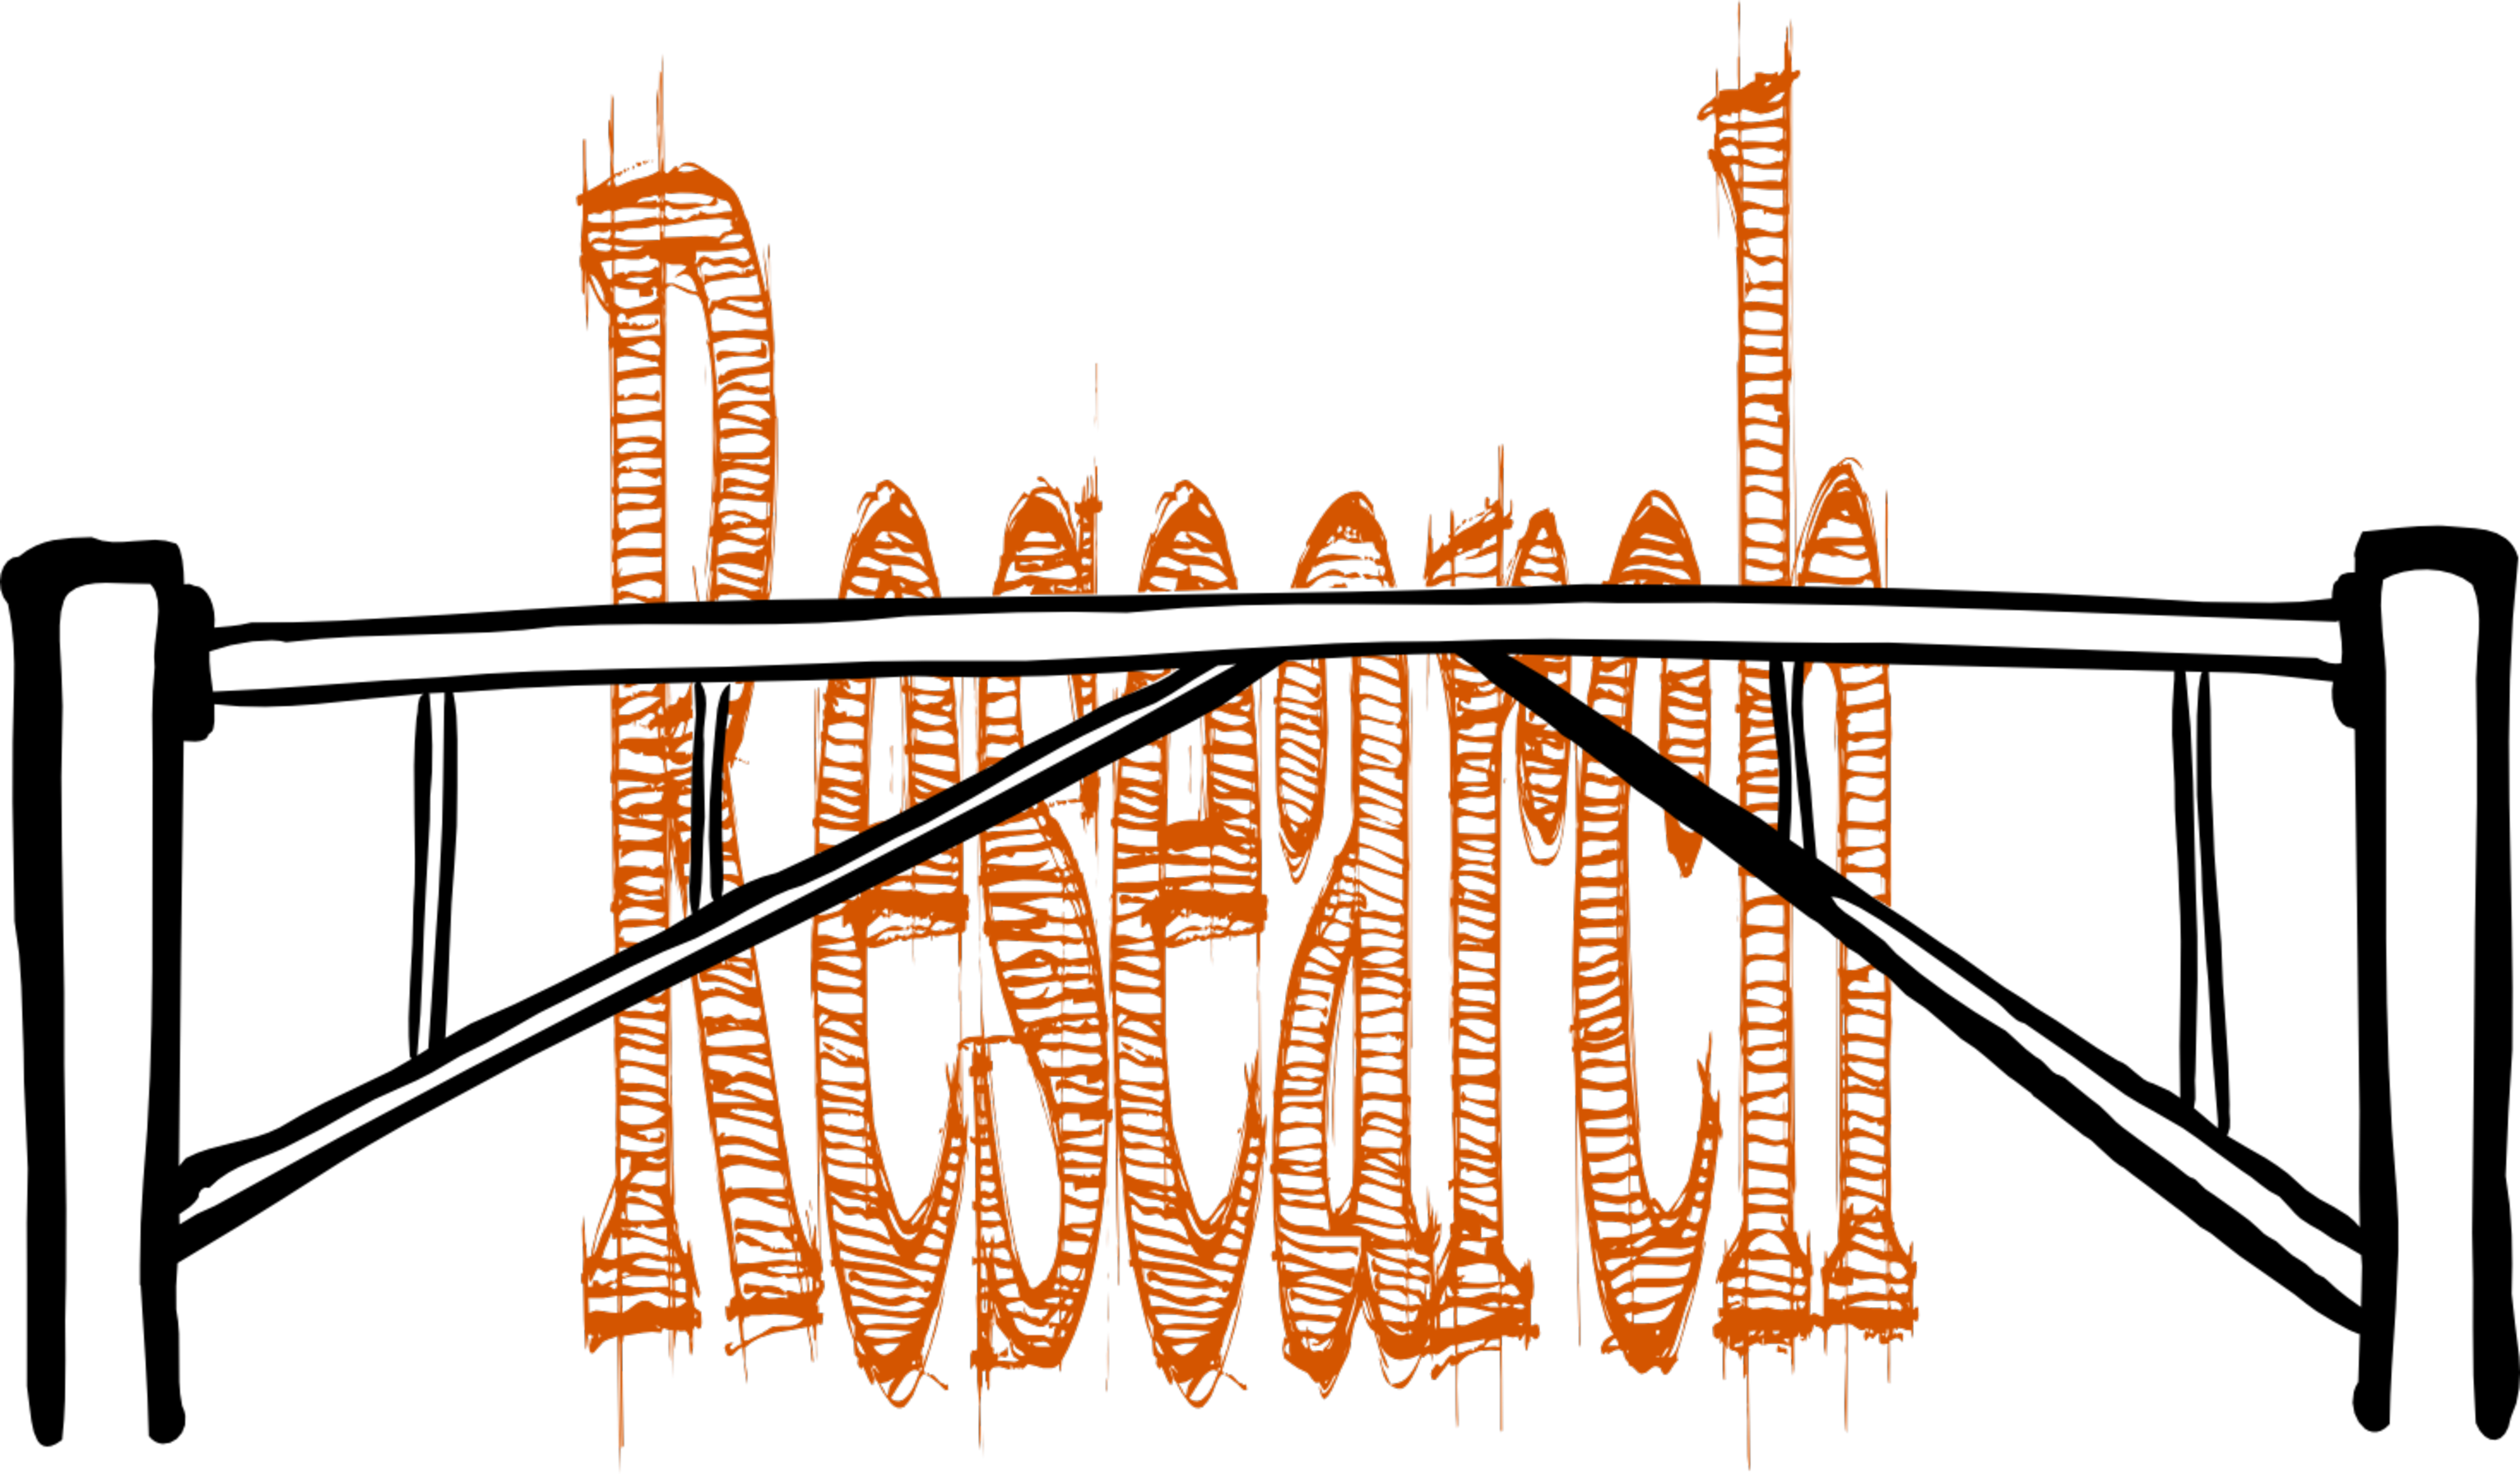
\includegraphics[height=.15\textheight]{./images/i2cvb/research.pdf}
      \end{figure}
      \vskip-4ex
      \begin{itemize}\tiny
      \item Democratization of the ability to research
      \end{itemize}
      \vskip1ex
    \end{block}
    \begin{block}{
\includegraphics[height=.04\textheight]{./images/i2cvb/i2cvb.pdf}\ Protagonists}
      \begin{figure}
        \centering
        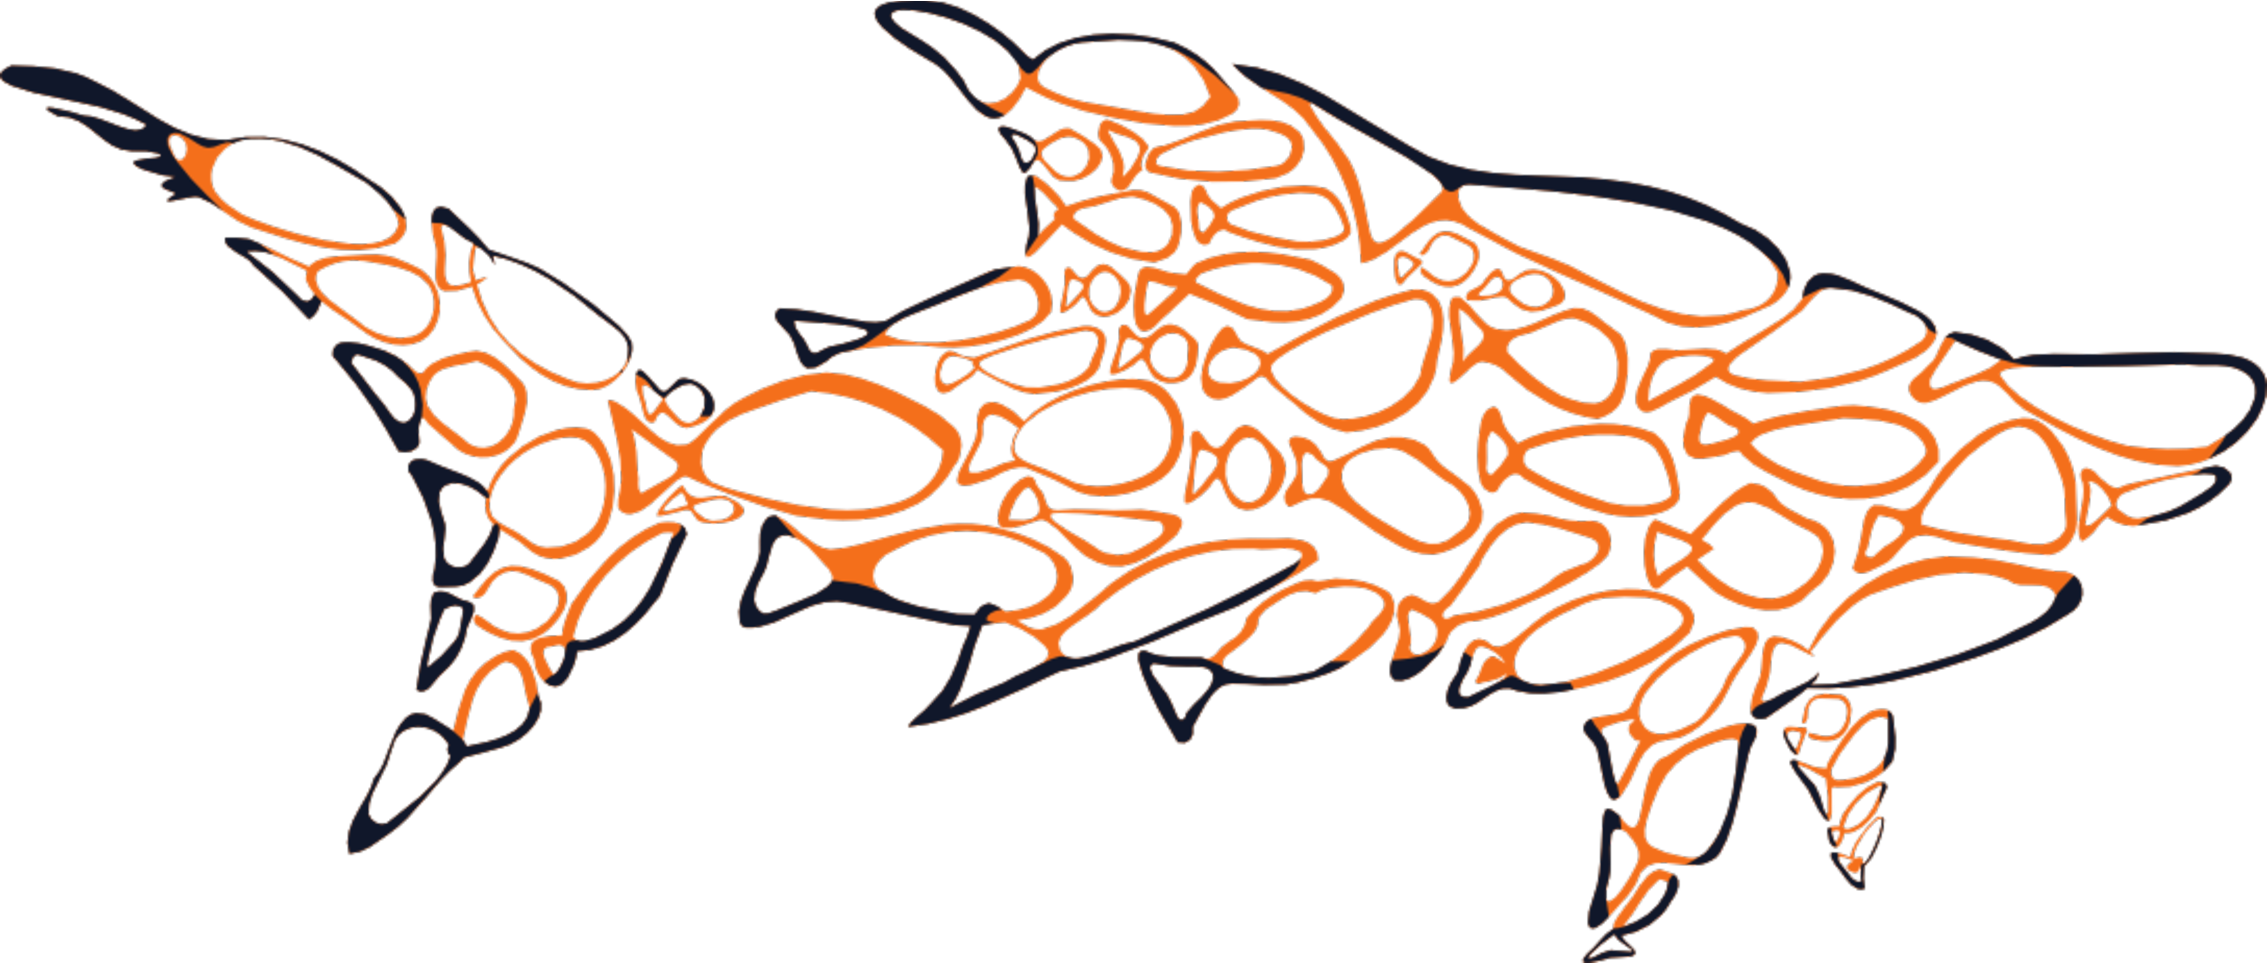
\includegraphics[height=.15\textheight]{./images/i2cvb/shark.pdf}
      \end{figure}
      \vskip-4ex
      \begin{itemize}\tiny
      \item Research groups and individuals from all walks of life to shape a transparent community
      \end{itemize}
    \end{block}
    \column{.5\textwidth}
    \begin{block}{
\includegraphics[height=.04\textheight]{./images/i2cvb/i2cvb.pdf}\ Mission}
      \begin{figure}
        \centering
        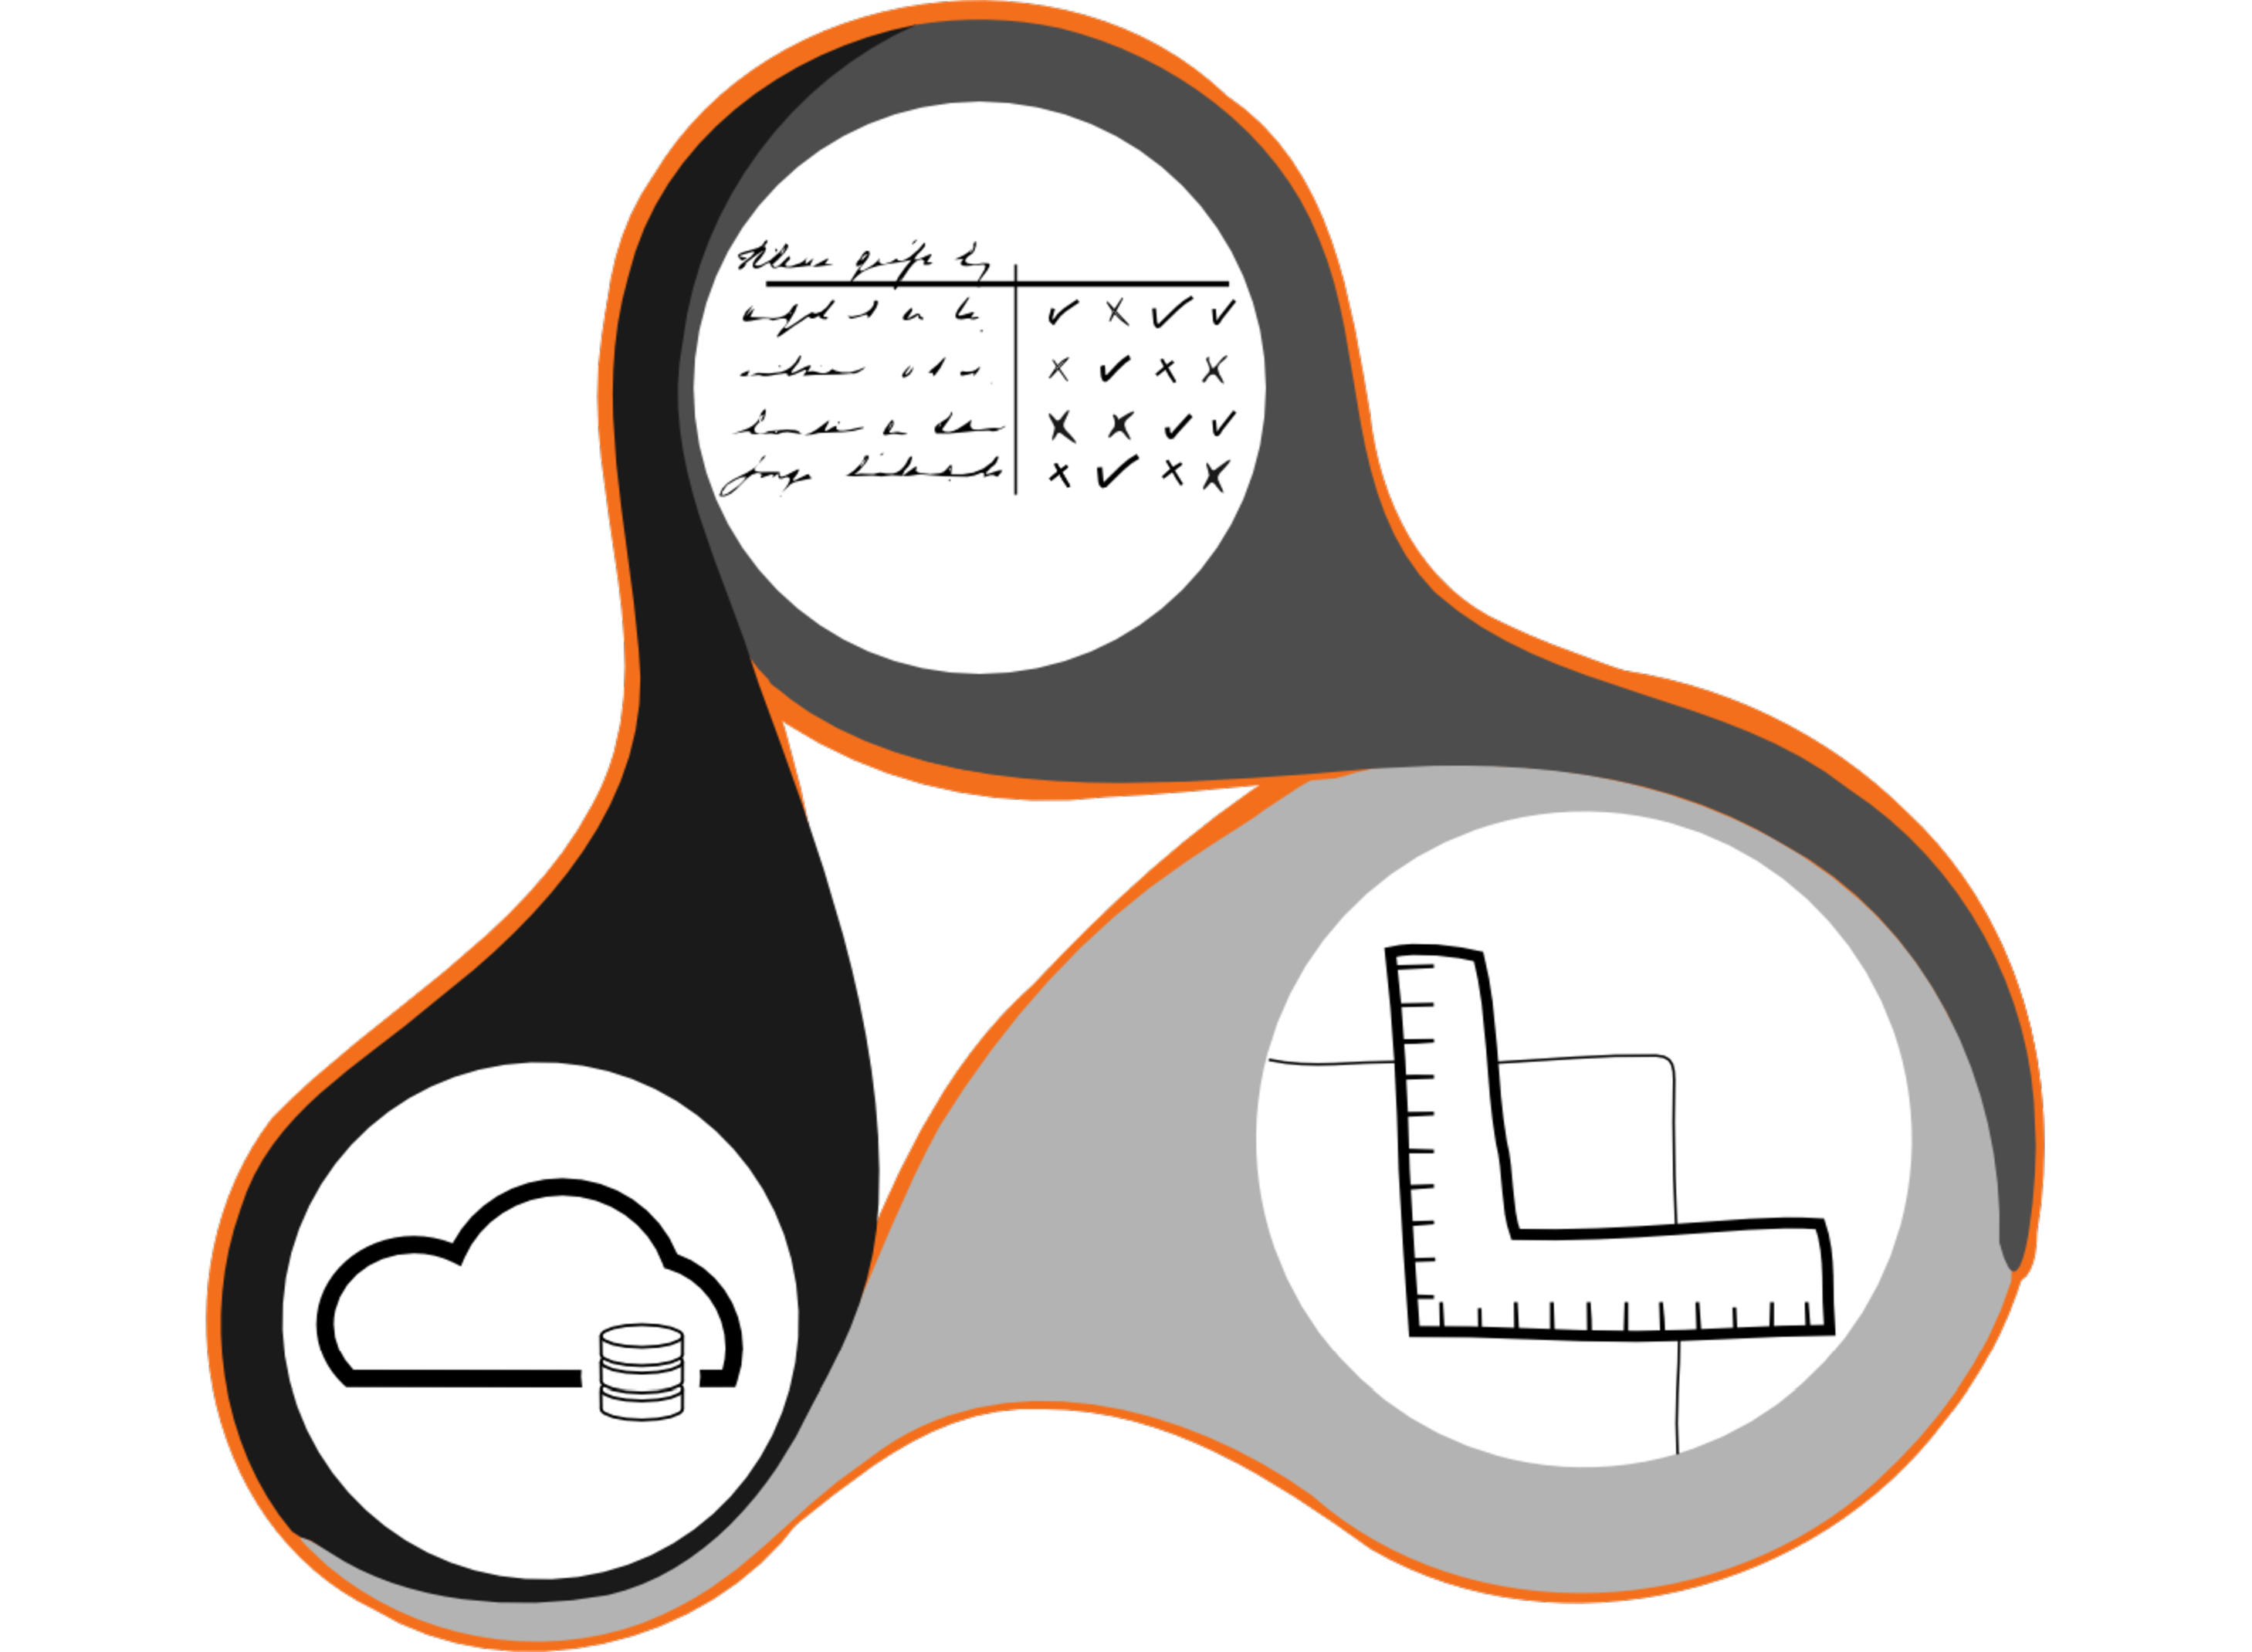
\includegraphics[height=.15\textheight]{./images/i2cvb/what.pdf}
      \end{figure}
      \vskip-4ex
      \begin{itemize}\tiny
      \item Open data; evaluation methods; comparison framework; reporting platform
      \end{itemize}
    \end{block}
    \begin{block}{
\includegraphics[height=.04\textheight]{./images/i2cvb/i2cvb.pdf}\ Strategy}
      \begin{figure}
        \centering
        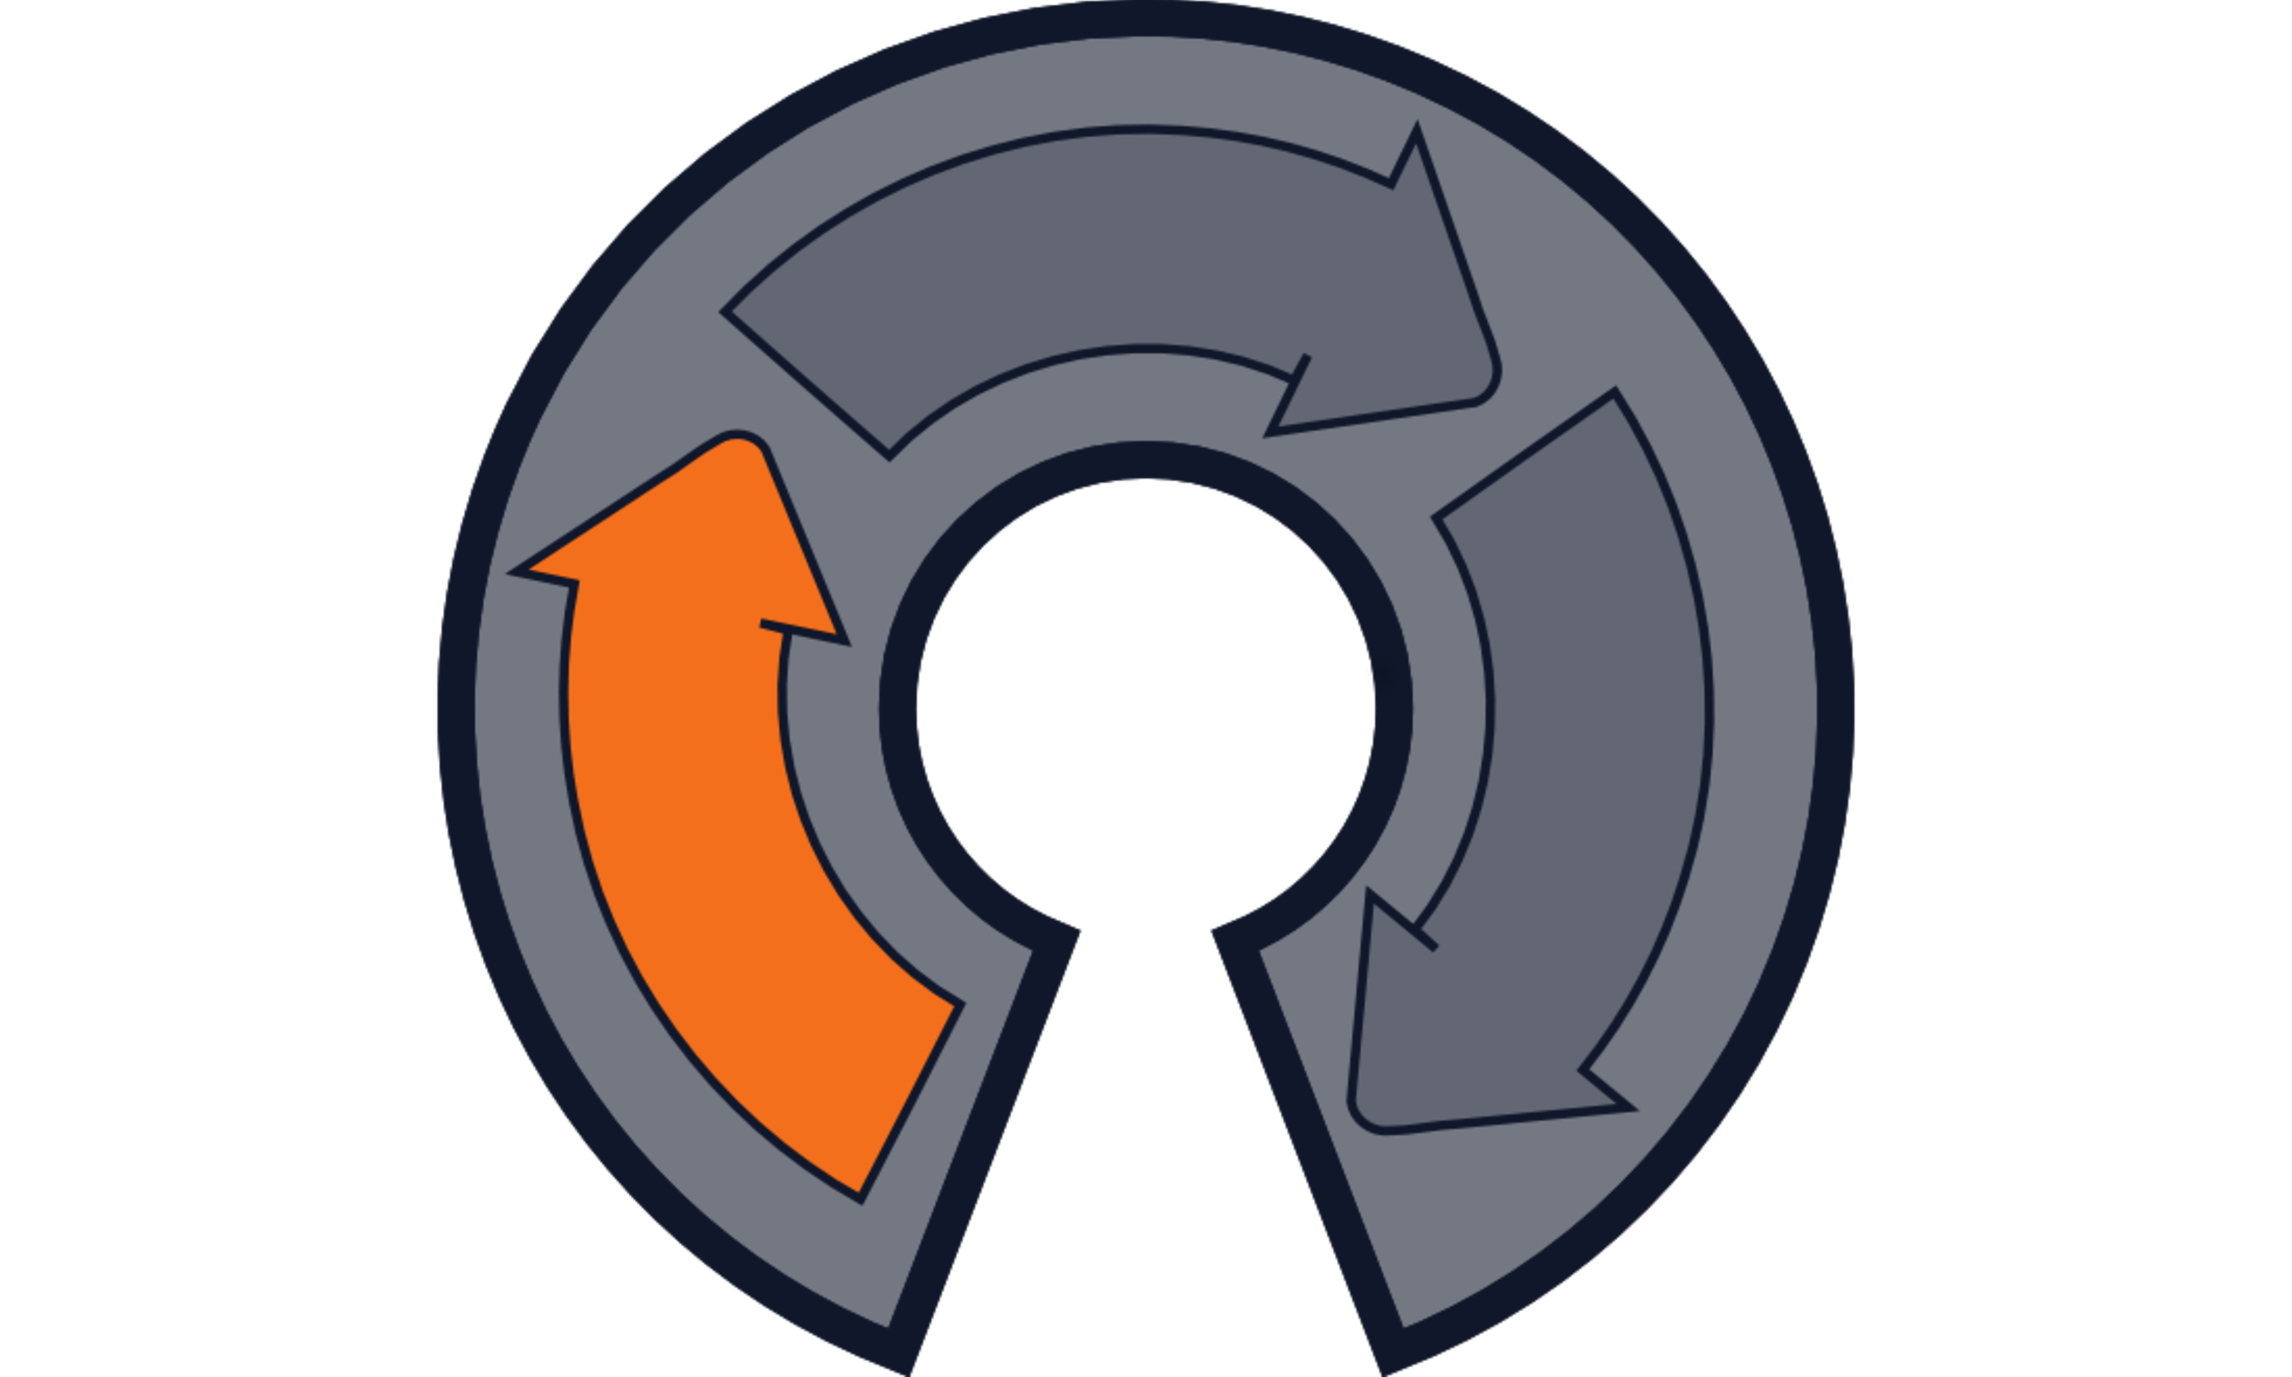
\includegraphics[height=.15\textheight]{./images/i2cvb/open.pdf}
      \end{figure}
      \vskip-4ex
      \begin{itemize}\tiny
      \item Transferring successful practises from Free Software and Quality Management
      \end{itemize}
      \vskip1ex
    \end{block}
  \end{columns}
\end{frame}

\subsection{Prostate dataset}

\begin{frame}
  \frametitle{I2CVB}
  \framesubtitle{Prostate dataset}
  \begin{block}{\small Multi-parametric MRI}\footnotesize
    \begin{itemize}
    \item Cohort of 20 patients
    \item T$_2$W MRI, DCE MRI \& ADC
    \item 3 Tesla whole body MRI without endorectal coil
    \end{itemize}
  \end{block}
  \begin{greenblock}{\small Ground-truth}\footnotesize
    \begin{itemize}
    \item Delineations: prostate - zones - CaP
    \item Healthy: 2 \textit{vs.} CaP: \{PZ: 13, CG: 3, PZ + CG: 2 \}
    \end{itemize}
  \end{greenblock}
\end{frame}

\end{document}